\section{Variables Aleatorias}

\mode<presentation>{
%---------------------------------------------------------------------slide----
\begin{frame}
\frametitle{Variables aleatorias}
\tableofcontents[sectionstyle=show/hide,hideothersubsections]
\end{frame}
}


%---------------------------------------------------------------------slide----
\begin{frame}
\frametitle{Variable aleatoria}
Cuando seleccionamos una muestra al azar de una población estamos realizando un experimento aleatorio y cualquier variable
estadística medida a partir de la muestra será una variable aleatoria porque sus valores dependerán del azar. 

\begin{definicion}[Variable Aleatoria] 
Una \emph{variable aleatoria} $X$ es una función que asocia un número real a cada elemento del
espacio muestral de un experimento aleatorio. \[ X:E\rightarrow \mathbb{R} \]

Al conjunto de posibles valores que puede tomar la variable aleatoria se le llama \emph{rango} o \emph{recorrido} de la variable.
\end{definicion}

En el fondo, una variable aleatoria es una variable cuyos valores provienen de la realización de un experimento aleatorio, y por tanto,
tendrá asociada una determinada distribución de probabilidad.

Un ejemplo de variable aleatoria es la que mide el resultado del lanzamiento de un dado.

\note{
Con este tema entramos de lleno en la inferencia estadística, que tiene por objeto construir modelos probabilísticos que
expliquen el comportamiento de las variables en las poblaciones. Estas variables se llaman variables aleatorias porque al medirlas en
la muestra obtenida al azar de la población, sus valores provienen de realizar un experimento aleatorio.  

\begin{definicion}[Variable Aleatoria] 
Una \emph{variable aleatoria} $X$ es una función que asocia un número real a cada elemento del
espacio muestral de un experimento aleatorio. \[ X:E\rightarrow \mathbb{R} \]

Al conjunto de posibles valores que puede tomar la variable aleatoria se le llama \emph{rango} o \emph{recorrido} de la variable.
\end{definicion}

Como los valores de una variable aleatoria provienen de la realización de un experimento aleatorio, 
tendrá asociada una determinada distribución de probabilidad. Nuestro objetivo es conocer lo mejor posible esa distribución de probabilidad
pero debemos recordar que cuando estudiemos una determinada variable,
normalmente no conoceremos con exactitud cómo se distribuyen sus valores en la población, ya que no podremos medir a todos los invididuos de
la misma. Por tanto, los modelos de distribución de probabilidad que utilizaremos para describir el comportamiento de las variables en las
poblaciones serán modelos aproximados. 

Un ejemplo de variable aleatoria es la que mide el resultado del lanzamiento de un dado.
}
\end{frame}


%---------------------------------------------------------------------slide----
\begin{frame}
\frametitle{Variable aleatoria}
Las variables aleatorias se clasifican en dos tipos:
\begin{description}
\item[Discretas (VAD):] Toman valores aislados (recorrido finito o infinito numerable).\\
Ejemplo. Número de hijos, número de accidentes, número de cigarrillos, etc. 
\item[Continuas (VAC):] Toman valores en un intervalo real.\\
Ejemplo. Peso, estatura, nivel de colesterol, tiempo de respuesta a un fármaco, etc. 
\end{description}

Los modelos probabilísticos de cada tipo de variables tienen características diferenciadas y por eso se estudiarán por separado. 

\note{
Las variables aleatorias se clasifican en dos tipos:
\begin{description}
\item[Discretas (VAD):] Toman valores aislados (recorrido finito o infinito numerable).\\
Ejemplo. Número de hijos, número de accidentes, número de cigarrillos, etc. 
\item[Continuas (VAC):] Toman valores en un intervalo real.\\
Ejemplo. Peso, estatura, nivel de colesterol, tiempo de respuesta a un fármaco, etc. 
\end{description}

Los modelos probabilísticos de cada tipo de variables tienen características diferenciadas y por eso se estudiarán por separado. 
}
\end{frame}


\subsection{Variables Aleatorias Discretas}

%---------------------------------------------------------------------slide----
\begin{frame}
\frametitle{Distribución de probabilidad de una variable discreta}
Como los valores de una variable aleatoria están asociados a los sucesos elementales del correspondiente experimento aleatorio, cada valor
tendrá asociada una probabilidad.
\begin{definicion}[Función de probabilidad]
La \emph{función de probabilidad} de una variable aleatoria discreta $X$ es una función $f(x)$ que asocia a cada valor su probabilidad
\[
f(x_i) = P(X=x_i).
\] 
\end{definicion} 

Las probabilidades también pueden acumularse, al igual que se acumulaban las frecuencias en las muestras.

\begin{definicion}[Función de distibución] 
La \emph{función de distribución} de una variable aleatoria discreta $X$ es una función $F(x)$
que asocia a cada valor $x_i$ la probabilidad de que la variable tome un valor menor o igual que dicho valor. 
\[
F(x_i) = P(X\leq x_i) = f(x_1)+\cdots +f(x_i).
\]
\end{definicion} 

\note{
Como los valores de una variable aleatoria están asociados a los sucesos elementales del correspondiente experimento aleatorio, cada valor
tendrá asociada una probabilidad.
\begin{definicion}[Función de probabilidad]
La \emph{función de probabilidad} de una variable aleatoria discreta $X$ es una función $f(x)$ que asocia a cada valor su probabilidad
\[
f(x_i) = P(X=x_i).
\] 
\end{definicion}  

Al igual que se acumulaban las frecuencias en las muestras, tiene sentido acumular probabilidades en las poblaciones. De eso se encarga la
función de distribución.

\begin{definicion}[Función de distibución] 
La \emph{función de distribución} de una variable aleatoria discreta $X$ es una función $F(x)$
que asocia a cada valor $x_i$ la probabilidad de que la variable tome un valor menor o igual que dicho valor. 
\[
F(x_i) = P(X\leq x_i) = f(x_1)+\cdots +f(x_i).
\]
\end{definicion} 
}
\end{frame}


%---------------------------------------------------------------------slide----
\begin{frame}
\frametitle{Distribución de probabilidad de una variable discreta}
Al recorrido de la variable, junto a su función de probabilidad o de distribución, se le llama \structure{\textbf{Distribución de probabilidad}} de la variable.

Tanto la función de probabilidad como la de distribución suelen representarse en forma de tabla
\[
\begin{array}{|c|cccc|c|}
\hline
X & x_1 & x_2 & \cdots & x_n & \sum\\ \hline
f(x) & f(x_1) & f(x_2) & \cdots & f(x_n) & 1\\
\hline
F(x) & F(x_1) & F(x_2) & \cdots & F(x_n) =1 &\multicolumn{1}{|c}{} \\
\cline{1-5}
\end{array}
\]

Al igual que la distribución de frecuencias de una variable reflejaba cómo se distribuían los valores de la variable en una muestra, la
distribución de probabilidad de una variable aleatoria sirve para reflejar cómo se distribuyen los valores de dicha variable en toda la
población.

\note{
Al recorrido de la variable, junto a su función de probabilidad o de distribución, se le llama \structure{\textbf{Distribución de probabilidad}} de la variable.

Tanto la función de probabilidad como la de distribución suelen representarse en forma de tabla
\[
\begin{array}{|c|cccc|c|}
\hline
X & x_1 & x_2 & \cdots & x_n & \sum\\ \hline
f(x) & f(x_1) & f(x_2) & \cdots & f(x_n) & 1\\
\hline
F(x) & F(x_1) & F(x_2) & \cdots & F(x_n) =1 &\multicolumn{1}{|c}{} \\
\cline{1-5}
\end{array}
\]

Al igual que la distribución de frecuencias de una variable reflejaba cómo se distribuían los valores de la variable en una muestra, la
distribución de probabilidad de una variable aleatoria sirve para reflejar cómo se distribuyen los valores de dicha variable en toda la
población.
}
\end{frame}


%---------------------------------------------------------------------slide----
\begin{frame}
\frametitle{Distribución de probabilidad de una variable discreta}
\framesubtitle{Ejemplo del lanzamiento de dos monedas}
Sea $X$ la variable aleatoria que mide el número de caras en el lanzamiento de dos monedas. 


El árbol de probabilidad asociado al experimento es 
\begin{center}
\scalebox{0.8}{
\psset{treesep=0.5cm, levelsep=2.5cm, tpos=0.7}
\renewcommand{\psedge}[2]{\ncdiag[armA=0.8cm,angleA=180,angleB=0,armB=0cm]{#2}{#1}} 
\pstree[treemode=R, nodesep=1pt]{\Tp*}{
	\pstree[linestyle=none]{\TR[edge=none]{1ª Moneda}}{
		\pstree[levelsep=2cm]{\TR{2ª Moneda}}{
			\pstree{\TR{$E$}}{
				\pstree{\TR{$P$}}{\TR{$X$}}
			}
		}
	}
	\pstree{\TR{C}\taput{\scriptsize $0.5$}}{
		\pstree[linestyle=none,levelsep=2cm]{\TR{C}\taput{\scriptsize $0.5$}}{
			\pstree{\TR{(C,C)}}{
				\pstree{\TR{$0.25$}}{\TR{$2$}}
			}
		}
		\pstree[linestyle=none,levelsep=2cm]{\TR{X}\taput{\scriptsize $0.5$}}{
			\pstree{\TR{(C,X)}}{
				\pstree{\TR{$0.25$}}{\TR{$1$}}
			}
		}
	}
	\pstree{\TR{X}\taput{\scriptsize $0.5$}}{
		\pstree[linestyle=none,levelsep=2cm]{\TR{C}\taput{\scriptsize $0.5$}}{
			\pstree{\TR{(X,C)}}{
				\pstree{\TR{$0.25$}}{\TR{$1$}}
			}
		}
		\pstree[linestyle=none,levelsep=2cm]{\TR{X}\taput{\scriptsize $0.5$}}{
			\pstree{\TR{(X,X)}}{
				\pstree{\TR{$0.25$}}{\TR{$0$}}
			}
		}
	}
	\pstree[linestyle=none]{\Tp[edge=none]}{\Tp}
}
}
\end{center}
y según esto, su distribución de probabilidad es
\[
\begin{array}{|c|ccc|}
\hline
X & 0 & 1 & 2\\ \hline
f(x) & 0.25 & 0.5 & 0.25\\
\hline
F(x) & 0.25 & 0.75 & 1 \\
\hline 
\end{array}
\qquad
F(x) =
\begin{cases}
0 & \mbox{si $x<0$}\\
0.25 & \mbox{si $0\leq x< 1$}\\
0.75 & \mbox{si $1\leq x< 2$}\\
1 & \mbox{si $x\geq 2$}
\end{cases}
\]
\end{frame}


%---------------------------------------------------------------------slide----
\begin{frame}
\frametitle{Gráficos de la funciones de probabilidad y distribución}
\framesubtitle{Ejemplo del lanzamiento de dos monedas}
\begin{center}
\begin{tabular}{cc}
Función de probabilidad & Función de distribución\\
\scalebox{0.5}{%% Input file name: /media/datos/ceu/docencia/materiales/estadistica/presentaciones/curso_estadistica/img/variables_aleatorias_discretas/funcion_probabilidad_lanzamiento_2_monedas.fig
%% FIG version: 3.2
%% Orientation: Landscape
%% Justification: Flush Left
%% Units: Inches
%% Paper size: A4
%% Magnification: 100.0
%% Resolution: 1200ppi

\begin{pspicture}(5.75cm,3.48cm)(16.66cm,13.45cm)
\psset{unit=0.8cm}
%%
%% Depth: 2147483647
%%
\newrgbcolor{mycolor0}{1.00 0.50 0.31}\definecolor{mycolor0}{rgb}{1.00,0.50,0.31}
\newgray{mycolor1}{0.74}\definecolor{mycolor1}{gray}{0.74}
%%
%% Depth: 100
%%
\psset{linestyle=none,fillstyle=solid,fillcolor=mycolor0}
\pscircle(10.61,10.88){0.1}
\pscircle(15.27,14.95){0.1}
\pscircle(19.94,10.88){0.1}
\psset{linestyle=solid,linecolor=black,fillstyle=none}
\psline(10.61,6.47)(19.94,6.47)
\psline(10.61,6.47)(10.61,6.26)
\psline(15.27,6.47)(15.27,6.26)
\psline(19.94,6.47)(19.94,6.26)
\rput(10.61,5.71){0.0}
\rput(15.27,5.71){1.0}
\rput(19.94,5.71){2.0}
\psline(10.23,6.80)(10.23,14.95)
\psline(10.23,6.80)(10.02,6.80)
\psline(10.23,8.43)(10.02,8.43)
\psline(10.23,10.06)(10.02,10.06)
\psline(10.23,11.69)(10.02,11.69)
\psline(10.23,13.32)(10.02,13.32)
\psline(10.23,14.95)(10.02,14.95)
\rput{90}(9.73,6.80){0.0}
\rput{90}(9.73,8.43){0.1}
\rput{90}(9.73,10.06){0.2}
\rput{90}(9.73,11.69){0.3}
\rput{90}(9.73,13.32){0.4}
\rput{90}(9.73,14.95){0.5}
\psline(10.23,6.47)(20.31,6.47)(20.31,15.28)(10.23,15.28)(10.23,6.47)
\rput(15.27,15.99){Lanzamiento de dos monedas}
\rput(15.27,4.86){Nº de caras}
\rput{90}(8.88,10.88){Probabilidad}
\psset{linecolor=mycolor1}
\psline(10.23,6.80)(20.31,6.80)
\end{pspicture}
%% End
}
&
\scalebox{0.5}{%% Input file name: /media/datos/ceu/docencia/materiales/estadistica/presentaciones/curso_estadistica/img/variables_aleatorias_discretas/funcion_distribucion_lanzamiento_2_monedas.fig
%% FIG version: 3.2
%% Orientation: Landscape
%% Justification: Flush Left
%% Units: Inches
%% Paper size: A4
%% Magnification: 100.0
%% Resolution: 1200ppi

\begin{pspicture}(5.87cm,3.48cm)(16.66cm,13.45cm)
\psset{unit=0.8cm}
%%
%% Depth: 2147483647
%%
\newrgbcolor{mycolor0}{1.00 0.50 0.31}\definecolor{mycolor0}{rgb}{1.00,0.50,0.31}
\newgray{mycolor1}{0.74}\definecolor{mycolor1}{gray}{0.74}
\newrgbcolor{mycolor2}{0.25 0.41 0.88}\definecolor{mycolor2}{rgb}{0.25,0.41,0.88}
%%
%% Depth: 100
%%
\psset{linestyle=none,fillstyle=solid,fillcolor=mycolor0}
\pscircle(10.61,8.84){0.1}
\pscircle(15.27,12.91){0.1}
\pscircle(19.94,14.95){0.1}
\psset{linestyle=solid,linecolor=black,fillstyle=none}
\psline(10.61,6.47)(19.94,6.47)
\psline(10.61,6.47)(10.61,6.26)
\psline(15.27,6.47)(15.27,6.26)
\psline(19.94,6.47)(19.94,6.26)
\rput(10.61,5.71){0.0}
\rput(15.27,5.71){1.0}
\rput(19.94,5.71){2.0}
\psline(10.23,6.80)(10.23,14.95)
\psline(10.23,6.80)(10.02,6.80)
\psline(10.23,8.43)(10.02,8.43)
\psline(10.23,10.06)(10.02,10.06)
\psline(10.23,11.69)(10.02,11.69)
\psline(10.23,13.32)(10.02,13.32)
\psline(10.23,14.95)(10.02,14.95)
\rput{90}(9.73,6.80){0.0}
\rput{90}(9.73,8.43){0.2}
\rput{90}(9.73,10.06){0.4}
\rput{90}(9.73,11.69){0.6}
\rput{90}(9.73,13.32){0.8}
\rput{90}(9.73,14.95){1.0}
\psline(10.23,6.47)(20.31,6.47)(20.31,15.28)(10.23,15.28)(10.23,6.47)
\rput(15.27,15.99){Lanzamiento de dos monedas}
\rput(15.27,4.86){Nº de caras}
\rput{90}(8.88,10.88){Probabilidad acumulada}
\psset{linecolor=mycolor1}
\psline(10.23,6.80)(20.31,6.80)
\psset{linewidth=0.0635,linecolor=mycolor2}
\psline(10.23,6.80)(10.61,6.80)(10.61,8.84)(15.27,8.84)(15.27,12.91)(19.94,12.91)(19.94,14.95)(20.31,14.95)
\end{pspicture}
%% End
}
\end{tabular}
\end{center}

\note{
Tanto la función de probabilidad como la de distribución también suelen representarse gráficamente, de igual modo que representabamos las
frecuencias muestrales.

Como se trata de variables discretas, el diagrama que se utiliza es el diagrama de barras o el diagrama de puntos, donde para cada valor se
levanta una barra con el valor de la función de probabilidad o con el valor de la función de distribución.

En el ejemplo de la variable que mide el número de caras al lanzar dos monedas, se tiene que la gráfica de la función de probabilidad es
la que aparece a la izquierda, mientras que la de la función de distribución es la de la derecha.
}
\end{frame}


%---------------------------------------------------------------------slide----
\begin{frame}
\frametitle{Estadísticos poblacionales}
Al igual que para describir las variables medidas en las muestras se utilizan estadísticos descriptivos, para describir determinadas
características de las variables aleatorias se utilizan también estadísticos poblacionales.

La definición de los estadísticos poblacionales es análoga a la de los muestrales, pero utilizando probabilidades en lugar de frecuencias
relativas.

Los más importantes son\footnote{Para distinguirlos de los muestrales se suelen representar con letras griegas}:
\begin{itemize}
\item \structure{Media o esperanza matemática}:
\[
\mu = E(X) = \sum_{i=1}^n x_i f(x_i)
\]
\item \structure{Varianza}:
\[
\sigma^2 = Var(X) = \sum_{i=1}^n x_i^2 f(x_i) -\mu^2
\]
\item \structure{Desviación típica}:
\[
\sigma = +\sqrt{\sigma^2}
\] 
\end{itemize}

\note{
Al igual que para describir las variables medidas en las muestras se utilizan estadísticos descriptivos, para describir determinadas
características de variables aleatorias se utilizan también estadísticos poblacionales.

Los estadísticos poblacionales se representan con letras griegas para distinguirlos de los muestrales, y su definición es análoga a la de
los muestrales, pero utilizando probabilidades en lugar de frecuencias relativas.

Por ejemplo, si definíamos la media muestral como la suma del producto de cada valor por su frecuencia relativa, la media poblacional, que
también se llama esperanza matemática, y se representa por $\mu$, se calcula como la suma del producto de cada valor de la variable por su
probabilidad. 

La varianza poblacional se calcula sumando los productos de los cuadrados de los valores de la variable por su probabilidad y restandole al
total de la suma la media poblacional al cuadrado. 

La desviación típica poblacional, como siempre, es la raíz cuadrada positiva de la varianza poblacional.

Otros estadísticos, se definen de forma similar a como lo hacíamos para muestras. Por ejemplo, la mediana será el valor cuya probabilidad
acumulada sea $0.5$. 
}

\end{frame}


%---------------------------------------------------------------------slide----
\begin{frame}
\frametitle{Estadísticos poblacionales}
\framesubtitle{Ejemplo de cálculo en el caso del lanzamiento de dos monedas}
En el ejemplo del lanzamiento de dos monedas, a partir de la distribución de probabilidad
\[
\begin{array}{|c|ccc|}
\hline
X & 0 & 1 & 2\\ \hline
f(x) & 0.25 & 0.5 & 0.25\\
\hline
F(x) & 0.25 & 0.75 & 1 \\
\hline 
\end{array}
\]
se pueden calcular fácilmente los estadísticos poblacionales:
\begin{align*}
\mu &= \sum_{i=1}^n x_i f(x_i) = 0\cdot 0.25 + 1\cdot 0.5 + 2\cdot 0.25 = 1 \mbox{ cara},\\
\sigma^2 &= \sum_{i=1}^n x_i^2 f(x_i) -\mu^2 = (0^0\cdot 0.25 + 1^2\cdot 0.5 + 2^2\cdot 0.25) - 1^2 = 0.5 \mbox{ caras}^2,\\
\sigma &= +\sqrt{0.5} = 0.71 \mbox{ caras}.
\end{align*} 

\note{
Veamos cómo calcular los principales estadísticos de la variable que medía el número de caras en el lanzamiento de dos monedas. 
}
\end{frame}


%---------------------------------------------------------------------slide----
\begin{frame}
\frametitle{Modelos de distribución de probabilidad}
En teoría, para obtener la distribución de probabilidad de una variable aleatoria en una población es necesario conocer el valor de la
variable en todos los individuos de la población, lo cual muchas veces es imposible.

Sin embargo, dependiendo de la naturaleza del experimento, a veces es posible obtener la distribución de probabilidad de una variable
aleatoria sin medirla en toda la población.

Dependiendo del tipo de experimento, existen diferentes modelos de distribución de probabilidad discretos. Los más habituales son:
\begin{itemize}
\item Distribución Uniforme.
\item Distribución Binomial.
\item Distribución de Poisson.
\end{itemize}

\note{
En teoría, para obtener la distribución de probabilidad de una variable aleatoria en una población es necesario conocer el valor de la
variable en todos los individuos de la población, lo cual muchas es imposible la mayoría de las veces.

Sin embargo, dependiendo de la naturaleza del experimento, a veces es posible obtener la distribución de probabilidad de una variable
aleatoria sin medirla en toda la población.

Dependiendo del tipo de experimento, existen diferentes modelos de distribución de probabilidad discretos. Los más habituales son:
\begin{itemize}
\item Distribución Uniforme.
\item Distribución Binomial.
\item Distribución de Poisson.
\end{itemize}

A continuación los veremos uno por uno.
}
\end{frame}


\subsection{Distribución Uniforme}

% ---------------------------------------------------------------------slide----
\begin{frame}
\frametitle{Distribución Uniforme $U_d(a,b)$}
Cuando por la simetría del experimento, todos los valores $a=x_1,\ldots,x_k=b$ de una variable discreta $X$ son igualmente probables, se
dice que la variable sigue un \emph{modelo de distribución uniforme}.

\begin{definicion}[Distribución uniforme $U_d(a,b)$]
Se dice que una variable aleatoria $X$ sigue un \emph{modelo de distribución uniforme} de parámetros $a,b$, y se nota,
$X\sim U_d(a,b)$, si su recorrido es $Re(X) = \{a=x_1,\ldots,x_k=b\}$, y su función de probabilidad vale
\[f(x_i)=\frac{1}{k}.\]
\end{definicion}

Su media y varianza valen
\[
\mu = \sum_{i=1}^{k}x_i\frac{1}{k} \qquad \sigma^2 =\sum_{i=1}^k (x_i-\mu)^2\frac{1}{k}.
\]

\note{
Cuando por la simetría del experimento, todos los valores $a=x_1,\ldots,x_k=b$ de una variable discreta $X$ son igualmente probables, se
dice que la variable sigue un \emph{modelo de distribución uniforme}.

\begin{definicion}[Distribución uniforme $U_d(a,b)$]
Se dice que una variable aleatoria $X$ sigue un \emph{modelo de distribución uniforme} de parámetros $a,b$, y se nota,
$X\sim U_d(a,b)$, si puede tomar $k$ valores distintos desde $a$ hasta $b$, es decir, su recorrido es $Re(X) = \{a=x_1,\ldots,x_k=b\}$, y su
función de probabilidad de cada uno de estos valores es la misma, es decir,  \[f(x_i)=\frac{1}{k}.\]
\end{definicion}

Su media, valdrá, por tanto, 
\[
\mu = \sum_{i=1}^{k}x_i\frac{1}{k}.
\]
y su varianza
\[
\sigma^2 =\sum_{i=1}^k (x_i-\mu)^2\frac{1}{k}.
\]
}
\end{frame}


%---------------------------------------------------------------------slide----
\begin{frame}
\frametitle{Distribución Uniforme $U_d(a,b)$}
\framesubtitle{Ejemplo del lanzamiento de un dado}
En el lanzamiento de un dado la variable que mide el número obtenido sigue un modelo de distribución uniforme
$U_d(1,6)$.
\begin{center}
\scalebox{0.65}{%% Input file name: funcion_probabilidad_uniforme.fig
%% FIG version: 3.2
%% Orientation: Landscape
%% Justification: Flush Left
%% Units: Inches
%% Paper size: A4
%% Magnification: 100.0
%% Resolution: 1200ppi
%% Include the following in the preamble:
%% \usepackage{textcomp}
%% End

\begin{pspicture}(5.45cm,3.48cm)(16.66cm,13.45cm)
\psset{unit=0.8cm}
%%
%% Depth: 2147483647
%%
\newrgbcolor{mycolor0}{1.00 0.50 0.31}\definecolor{mycolor0}{rgb}{1.00,0.50,0.31}
\newgray{mycolor1}{0.74}\definecolor{mycolor1}{gray}{0.74}
%%
%% Depth: 100
%%
\psset{linestyle=solid,linewidth=0.03175,linecolor=mycolor0}
\qdisk(10.61,13.59){0.1}
\qdisk(12.47,13.59){0.1}
\qdisk(14.34,13.59){0.1}
\qdisk(16.21,13.59){0.1}
\qdisk(18.07,13.59){0.1}
\qdisk(19.94,13.59){0.1}
\psset{linecolor=black,fillstyle=none}
\psline(10.61,6.47)(19.94,6.47)
\psline(10.61,6.47)(10.61,6.26)
\psline(12.47,6.47)(12.47,6.26)
\psline(14.34,6.47)(14.34,6.26)
\psline(16.21,6.47)(16.21,6.26)
\psline(18.07,6.47)(18.07,6.26)
\psline(19.94,6.47)(19.94,6.26)
\rput(10.61,5.71){1}
\rput(12.47,5.71){2}
\rput(14.34,5.71){3}
\rput(16.21,5.71){4}
\rput(18.07,5.71){5}
\rput(19.94,5.71){6}
\psline(10.23,6.80)(10.23,14.95)
\psline(10.23,6.80)(10.02,6.80)
\psline(10.23,8.84)(10.02,8.84)
\psline(10.23,10.88)(10.02,10.88)
\psline(10.23,12.91)(10.02,12.91)
\psline(10.23,14.95)(10.02,14.95)
\rput{90}(9.73,6.80){0.00}
\rput{90}(9.73,8.84){0.05}
\rput{90}(9.73,10.88){0.10}
\rput{90}(9.73,12.91){0.15}
\rput{90}(9.73,14.95){0.20}
\psline(10.23,6.47)(20.31,6.47)(20.31,15.28)(10.23,15.28)(10.23,6.47)
\rput(15.27,15.99){Función de probabilidad de una Uniforme $U(1,6)$}
\rput(15.27,4.86){$X$}
\rput{90}(8.88,10.88){Probabilidad $f(x)$}
\psset{linecolor=mycolor1}
\psline(10.23,6.80)(20.31,6.80)
\end{pspicture}
%% End
}
\end{center}

\note{
Un ejemplo sencillo de variable con distribución uniforme es la que mide el resultado del lanzamiento de un dado. Como puede tomar 6 valores
distintos del 1 al 6, su función de probabilidad es constante vale $1/6$ para cualquier valor, tal y como se aprecia en la gráfica.

El modelo de distribución uniforme es el más sencillo, pero resulta poco útil en la práctica ya que la equiprobabilidad no suele cumplirse
fuera de los juegos de azar.
}
\end{frame}


\subsection{Distribución Binomial}

%---------------------------------------------------------------------slide----
\begin{frame}
\frametitle{Distribución Binomial}
Sea un experimento aleatorio con las siguientes características:
\begin{itemize}
\item El experimento consiste en una secuencia de $n$ repeticiones de un mismo ensayo aleatorio.
\item Los ensayos se realizan bajo idénticas condiciones, y cada uno de ellos tiene únicamente dos posibles resultados,
que habitualmente se denotan por éxito ($A$) o fracaso ($\overline A$).
\item Los ensayos son independientes, por lo que el resultado de cualquier ensayo en particular no influye sobre el resultado de cualquier otro.
\item La probabilidad de éxito es idéntica para todos los ensayos y vale $P(A)=p$.
\end{itemize}
En estas condiciones, la variable aleatoria $X$ que mide le número de éxitos obtenidos en los $n$ ensayos sigue un
\emph{modelo de distribución binomial} de parámetros $n$ y $p$.

\note{
Mucho más habitual es el modelo binomial, que suele darse en experimentos aleatorios con las siguientes características:
\begin{itemize}
\item El experimento consiste en una secuencia de $n$ repeticiones de un mismo ensayo aleatorio. Por ejemplo, tirar 10 veces una moneda. 
\item Los ensayos se realizan bajo idénticas condiciones, y cada uno de ellos tiene únicamente dos posibles resultados,
que habitualmente se denotan por éxito ($A$) o fracaso ($\overline A$). Por ejemplo, medir en cada lanzamiento si sale cara (éxito) o si
sale cruz (fracaso).
\item Los ensayos son independientes, por lo que el resultado de cualquier ensayo en particular no influye sobre el resultado de cualquier
otro. Por ejemplo, el resultado de cada lanzamiento de la moneda no depende de los otros.
\item La probabilidad de éxito es idéntica para todos los ensayos y vale $P(A)=p$. Por ejemplo, la probabilidad de sacar cara es $0.5$ en
todos los lanzamientos. 
\end{itemize}
En estas condiciones, la variable aleatoria $X$ que mide le número de éxitos obtenidos en los $n$ ensayos sigue un
\emph{modelo de distribución binomial} de parámetros $n$ y $p$, donde $n$ era el número de repeticiones del ensayo y $p$ es la probabilidad
de lo que llamemos éxito. Así, la variable que mide el número de caras obtenidas en 10 lanzamientos de una moneda es sigue un modelo de
distribución binomial de parámetros $n=10$ y $p=0.5$.

}
\end{frame}


%---------------------------------------------------------------------slide----
\begin{frame}
\frametitle{Distribución Binomial $B(n,p)$}
\begin{definicion}[Distribución Binomial $(B(n,p)$]
Se dice que una variable aleatoria $X$ sigue un \emph{modelo de distribución binomial} de parámetros $n$ y $p$, si su recorrido es $Re(X) =
\{0,1,...,n\}$, y su función de probabilidad vale
\[
f(x) = \binom{n}{x}p^x(1-p)^{n-x} = \frac{n!}{x!(n-x)!}p^x(1-p)^{n-x}.
\]
\end{definicion}

Su media y varianza valen
\[
\mu = n\cdot p \qquad \sigma^2 = n\cdot p\cdot (1-p).
\]

\note{
Una variable con distribución binomial cumple que su recorrido va de $0$ a $n$ y su función de probablidad viene dada por la fórmula
\[
f(x) = \binom{n}{x}p^x(1-p)^{n-x}.
\]
donde el número combinatorio $\binom{n}{x}$ se define como $\frac{n!}{x!(n-x)!}$ y $n!$ es el producto de todos los números consecutivos
desde $1$ hasta $n$.

Se cumple además que su media es 
\[
\mu = n\cdot p.
\]
y su varianza
\[
\sigma^2 = n\cdot p\cdot (1-p).
\]
}
\end{frame}


%---------------------------------------------------------------------slide----
\begin{frame}
\frametitle{Distribución Binomial $B(n,p)$}
\framesubtitle{Ejemplo de 10 lanzamientos de una moneda}
La variable que mide el número de caras obtenidos al lanzar 10 veces una moneda sigue un modelo de distribución binomial $B(10,\,0.5)$.
\begin{center}
\scalebox{0.65}{%% Input file name: funcion_probabilidad_binomial.fig
%% FIG version: 3.2
%% Orientation: Landscape
%% Justification: Flush Left
%% Units: Inches
%% Paper size: A4
%% Magnification: 100.0
%% Resolution: 1200ppi
%% Include the following in the preamble:
%% \usepackage{textcomp}
%% End

\begin{pspicture}(5.45cm,3.48cm)(16.68cm,13.45cm)
\psset{unit=0.8cm}
%%
%% Depth: 2147483647
%%
\newrgbcolor{mycolor0}{1.00 0.50 0.31}\definecolor{mycolor0}{rgb}{1.00,0.50,0.31}
\newgray{mycolor1}{0.74}\definecolor{mycolor1}{gray}{0.74}
%%
%% Depth: 100
%%
\psset{linestyle=solid,linewidth=0.03175,linecolor=mycolor0}
\qdisk(10.61,6.83){0.1}
\qdisk(11.54,7.12){0.1}
\qdisk(12.47,8.23){0.1}
\qdisk(13.41,10.62){0.1}
\qdisk(14.34,13.49){0.1}
\qdisk(15.27,14.83){0.1}
\qdisk(16.21,13.49){0.1}
\qdisk(17.14,10.62){0.1}
\qdisk(18.07,8.23){0.1}
\qdisk(19.00,7.12){0.1}
\qdisk(19.94,6.83){0.1}
\psset{linecolor=black,fillstyle=none}
\psline(10.61,6.47)(19.94,6.47)
\psline(10.61,6.47)(10.61,6.26)
\psline(12.47,6.47)(12.47,6.26)
\psline(14.34,6.47)(14.34,6.26)
\psline(16.21,6.47)(16.21,6.26)
\psline(18.07,6.47)(18.07,6.26)
\psline(19.94,6.47)(19.94,6.26)
\rput(10.61,5.71){0}
\rput(12.47,5.71){2}
\rput(14.34,5.71){4}
\rput(16.21,5.71){6}
\rput(18.07,5.71){8}
\rput(19.94,5.71){10}
\psline(10.23,6.80)(10.23,14.95)
\psline(10.23,6.80)(10.02,6.80)
\psline(10.23,8.43)(10.02,8.43)
\psline(10.23,10.06)(10.02,10.06)
\psline(10.23,11.69)(10.02,11.69)
\psline(10.23,13.32)(10.02,13.32)
\psline(10.23,14.95)(10.02,14.95)
\rput{90}(9.73,6.80){0.00}
\rput{90}(9.73,8.43){0.05}
\rput{90}(9.73,10.06){0.10}
\rput{90}(9.73,11.69){0.15}
\rput{90}(9.73,13.32){0.20}
\rput{90}(9.73,14.95){0.25}
\psline(10.23,6.47)(20.31,6.47)(20.31,15.28)(10.23,15.28)(10.23,6.47)
\rput(15.27,15.99){Función de probabilidad de una binomial $B(10,0.5)$}
\rput(15.27,4.86){$X$}
\rput{90}(8.88,10.88){Probabilidad $f(x)$}
\psset{linecolor=mycolor1}
\psline(10.23,6.80)(20.31,6.80)
\end{pspicture}
%% End
}
\end{center}

\note{
Ya hemos visto que la variable que mide el número de caras obtenidos al lanzar 10 veces una moneda sigue un modelo de distribución binomial
$B(10,\,0.5)$. 

La gráfica de su función de probabilidad es esta. En ella se puede observar como se reparte la probabilidad entre los distintos valores que
van de 0 a 10. Obsérvese como el 0 y el 10 tienen probabilidades muy bajas, ya que es muy difícil que al tirar diez veces una moneda no se
obtenga ninguna cara, lo mismo que obtener 10 caras. Lo más probable, como se aprecia en el gráfico, es sacar 5 caras, que además es su
media.
}
\end{frame}


%---------------------------------------------------------------------slide----
\begin{frame}
\frametitle{Distribución Binomial $B(n,p)$}
\framesubtitle{Ejemplo de 10 lanzamientos de una monedas}
Sea $X\sim B(10,\,0.5)$ la variable que mide el número de caras en 10 lanzamientos de una moneda. Entonces:
\begin{itemize}
\item La probabilidad de sacar 4 caras es
\[
f(4) = \binom{10}{4}0.5^4 (1-0.5)^{10-4} = \frac{10!}{4!6!}0.5^40.5^6 = 210\cdot 0.5^{10} = 0.2051.
\]
\item La probabilidad de sacar dos o menos caras es
\begin{align*}
F(2) &= f(0) +f(1) + f(2) =\\
&= \binom{10}{0}0.5^0 (1-0.5)^{10-0} + \binom{10}{1}0.5^1 (1-0.5)^{10-1} + \binom{10}{2}0.5^2 (1-0.5)^{10-2} =\\
&= 0.0547.
\end{align*}
\item Y el número esperado de caras es 
\[ \mu = 10\cdot 0.5 = 5 \mbox{ caras}.\]   
\end{itemize}

\note{
Conocer la fórmula de la función de probabilidad de la binomial facilita mucho el cálculo de probabilidades para esta variable. Por ejemplo,
\begin{itemize}
\item La probabilidad de sacar 4 caras es
\[
f(4) = \binom{10}{4}0.5^4 (1-0.5)^{10-4} = \frac{10!}{4!6!}0.5^40.5^6 = 210\cdot 0.5^{10} = 0.2051.
\]
\item La probabilidad de sacar dos o menos caras es
\begin{align*}
F(2) &= f(0) +f(1) + f(2) =\\
&= \binom{10}{0}0.5^0 (1-0.5)^{10-0} + \binom{10}{1}0.5^1 (1-0.5)^{10-1} + \binom{10}{2}0.5^2 (1-0.5)^{10-2} =\\
&= 0.0547.
\end{align*}
\item Y el número esperado de caras, es decir, la media es 
\[ \mu = 10\cdot 0.5 = 5 \mbox{ caras}.\]   
\end{itemize}
}
\end{frame}


%---------------------------------------------------------------------slide----
\begin{frame}
\frametitle{Distribución Binomial $B(n,p)$}
\framesubtitle{Ejemplo de una muestra aleatoria con reemplazamiento}
Dada una población con un 40\% de hombres y un 60\% de mujeres, la variable que mide el número de mujeres en una muestra
aleatoria de tamaño 3, sigue una distribución binomial $X\sim B(3,\,0.6)$.

\begin{center}
\scalebox{0.7}{
\psset{treesep=0.4cm, levelsep=2cm, tpos=0.7}
\renewcommand{\psedge}[2]{\ncdiag[armA=0.8cm,angleA=180,angleB=0,armB=0cm]{#2}{#1}} 
\pstree[treemode=R, nodesep=1pt]{\Tp*}{
	\pstree[linestyle=none]{\TR[edge=none]{1ª Persona}}{
		\pstree{\TR{2ª Persona}}{
			\pstree[thislevelsep=1.5cm]{\TR{3ª Persona}}{
				\pstree[thislevelsep=1.5cm]{\TR{$E$}}{
					\pstree[thislevelsep=1.5cm]{\TR{$X$}}{\TR{$P$}}
				}
			}
		}
	}
	\pstree{\TR{H}\taput{\scriptsize $0.4$}}{
		\pstree{\TR{H}\taput{\scriptsize $0.4$}}{
			\pstree[linestyle=none,thislevelsep=1.5cm]{\TR{H}\taput{\scriptsize $0.4$}}{
				\pstree[thislevelsep=1.5cm]{\TR{(H,H,H)}}{
					\pstree[thislevelsep=1.5cm]{\TR{\uncover<2->{0}}}{\TR{$0.4^3$}}
				}
			}
			\pstree[linestyle=none,thislevelsep=1.5cm]{\TR{M}\taput{\scriptsize $0.6$}}{
				\pstree[thislevelsep=1.5cm]{\TR{(H,H,M)}}{
					\pstree[thislevelsep=1.5cm]{\TR{\uncover<3->{1}}}{\TR{$0.6\cdot0.4^2$}}
				}
			}
		}
		\pstree{\TR{M}\taput{\scriptsize $0.6$}}{
			\pstree[linestyle=none,thislevelsep=1.5cm]{\TR{H}\taput{\scriptsize $0.4$}}{
				\pstree[thislevelsep=1.5cm]{\TR{(H,M,H)}}{
					\pstree[thislevelsep=1.5cm]{\TR{\uncover<3->{1}}}{\TR{$0.6\cdot 0.4^2$}}
				}
			}
			\pstree[linestyle=none,thislevelsep=1.5cm]{\TR{M}\taput{\scriptsize $0.6$}}{
				\pstree[thislevelsep=1.5cm]{\TR{(H,M,M)}}{
					\pstree[thislevelsep=1.5cm]{\TR{\uncover<4->{2}}}{\TR{$0.6^2\cdot 0.4$}}
				}
			}
		}	
	}
	\pstree{\TR{M}\taput{\scriptsize $0.6$}}{
		\pstree{\TR{H}\taput{\scriptsize $0.4$}}{
			\pstree[linestyle=none,thislevelsep=1.5cm]{\TR{H}\taput{\scriptsize $0.4$}}{
				\pstree[thislevelsep=1.5cm]{\TR{(M,H,H)}}{
					\pstree[thislevelsep=1.5cm]{\TR{\uncover<3->{1}}}{\TR{$0.6\cdot 0.4^2$}}
				}
			}
			\pstree[linestyle=none,thislevelsep=1.5cm]{\TR{M}\taput{\scriptsize $0.6$}}{
				\pstree[thislevelsep=1.5cm]{\TR{(M,H,M)}}{
					\pstree[thislevelsep=1.5cm]{\TR{\uncover<4->{2}}}{\TR{$0.6^2\cdot 0.4$}}
				}
			}
		}
		\pstree{\TR{M}\taput{\scriptsize $0.6$}}{
			\pstree[linestyle=none,thislevelsep=1.5cm]{\TR{H}\taput{\scriptsize $0.4$}}{
				\pstree[thislevelsep=1.5cm]{\TR{(M,M,H)}}{
					\pstree[thislevelsep=1.5cm]{\TR{\uncover<4->{2}}}{\TR{$0.6^2\cdot 0.4$}}
				}
			}
			\pstree[linestyle=none,thislevelsep=1.5cm]{\TR{M}\taput{\scriptsize $0.6$}}{
				\pstree[thislevelsep=1.5cm]{\TR{(M,M,M)}}{
					\pstree[thislevelsep=1.5cm]{\TR{\uncover<5->{3}}}{\TR{$0.6^3$}}
				}
			}
		}	
	}
	\pstree[linestyle=none]{\Tp[edge=none]}{\Tp}
}
}
\end{center}

\scalebox{0.9}{
\[
\renewcommand{\arraystretch}{1.5}
\begin{array}{lll}
\uncover<2->{f(0)=\binom{3}{0}0.6^0(1-0.6)^{3-0}= 0.4^3,} & \quad & 
\uncover<3->{f(1)=\binom{3}{1}0.6^1(1-0.6)^{3-1}= 3\cdot 0.6\cdot 0.4^2,}\\
\uncover<4->{f(2)=\binom{3}{2}0.6^2(1-0.6)^{3-2}= 3\cdot 0.6^2\cdot 0.4,} & & 
\uncover<5->{f(3)=\binom{3}{3}0.6^3(1-0.6)^{3-3}= 0.6^3.}
\end{array}
\]
}
\end{frame}


\subsection{Distribución de Poisson}

% ---------------------------------------------------------------------slide----
\begin{frame}
\frametitle{Distribución de Poisson}
Sea un experimento aleatorio con las siguientes características:
\begin{itemize}
\item El experimento consiste en observar la aparición de fenómenos puntuales sobre un soporte continuo, ya sea espacial o temporal. Por
ejemplo: averías de máquinas en un espacio de tiempo, recepción de llamadas en una centralita, nº de linfocitos en un volumen de
sangre,etc.
\item El experimento produce, a largo plazo, un número medio constante de fenómenos puntuales por unidad de soporte continuo que llamaremos
$\lambda$.
\end{itemize}
En estas circunstancias, la variable aleatoria $X$ que mide el número de ocurrencias del fenómeno por unidad de soporte
continuo sigue un \emph{modelo de distribución de Poisson} de parámetro $\lambda$.

\note{
La distribución de Poisson surge en experimentos aleatorios con las siguientes características:
\begin{itemize}
\item El experimento consiste en observar la aparición de fenómenos puntuales sobre un soporte continuo, ya sea espacial o temporal. Por
ejemplo: averías de máquinas en un espacio de tiempo, recepción de llamadas en una centralita, nº de linfocitos en un volumen de
sangre,etc.
\item Además el experimento produce, a largo plazo, un número medio constante de fenómenos puntuales por unidad de soporte continuo que
llamaremos $\lambda$.
\end{itemize}
En estas circunstancias, la variable aleatoria $X$ que mide el número de ocurrencias del fenómeno por unidad de soporte
continuo sigue un \emph{modelo de distribución de Poisson} de parámetro $\lambda$.
}
\end{frame}


%---------------------------------------------------------------------slide----
\begin{frame}
\frametitle{Distribución de Poisson $P(\lambda)$}
\begin{definicion}[Distribución de Poisson $P(\lambda)$]
Se dice que una variable aleatoria $X$ sigue un \emph{modelo de distribución de Poisson} de parámetro $\lambda$ si su recorrido es $Re(X) = \{0,1,...,\infty\}$, y su función de probabilidad vale
\[
f(x) = e^{-\lambda}\frac{\lambda^x}{x!}.
\]
\end{definicion}

Su media y varianza valen
\[
\mu = \lambda \qquad \sigma^2 = \lambda.
\]

\note{
Una variable aleatoria con distribución de Poisson de parámetro $\lambda$ puede tomar valores de $0$ a $\infty$, y
su función de probabilidad viende dada por la fórmula
\[
f(x) = e^{-\lambda}\frac{\lambda^x}{x!}.
\]

Además, tanto su media como su varianza valen $\lambda$.
}
\end{frame}


%---------------------------------------------------------------------slide----
\begin{frame}
\frametitle{Distribución de Poisson $P(\lambda)$}
\framesubtitle{Ejemplo del número de ingresos en un hospital}
Sea un hospital en el que se producen por término medio 4 ingresos diarios. Entonces la variable aleatoria $X$ que mide el número de
ingresos en un día sigue un modelo de distribución de Poisson $X\sim P(4)$.
\begin{center}
\scalebox{0.63}{%% Input file name: funcion_probabilidad_poisson.fig
%% FIG version: 3.2
%% Orientation: Landscape
%% Justification: Flush Left
%% Units: Inches
%% Paper size: A4
%% Magnification: 100.0
%% Resolution: 1200ppi
%% Include the following in the preamble:
%% \usepackage{textcomp}
%% End

\begin{pspicture}(5.45cm,3.48cm)(16.66cm,13.45cm)
\psset{unit=0.8cm}
%%
%% Depth: 2147483647
%%
\newrgbcolor{mycolor0}{1.00 0.50 0.31}\definecolor{mycolor0}{rgb}{1.00,0.50,0.31}
\newgray{mycolor1}{0.74}\definecolor{mycolor1}{gray}{0.74}
%%
%% Depth: 100
%%
\psset{linestyle=solid,linewidth=0.03175,linecolor=mycolor0}
\qdisk(10.61,7.55){0.1}
\qdisk(11.39,9.79){0.1}
\qdisk(12.16,12.77){0.1}
\qdisk(12.94,14.76){0.1}
\qdisk(13.72,14.76){0.1}
\qdisk(14.49,13.17){0.1}
\qdisk(15.27,11.05){0.1}
\qdisk(16.05,9.23){0.1}
\qdisk(16.83,8.01){0.1}
\qdisk(17.60,7.34){0.1}
\qdisk(18.38,7.01){0.1}
\qdisk(19.16,6.88){0.1}
\qdisk(19.94,6.83){0.1}
\psset{linecolor=black,fillstyle=none}
\psline(10.61,6.47)(19.94,6.47)
\psline(10.61,6.47)(10.61,6.26)
\psline(12.16,6.47)(12.16,6.26)
\psline(13.72,6.47)(13.72,6.26)
\psline(15.27,6.47)(15.27,6.26)
\psline(16.83,6.47)(16.83,6.26)
\psline(18.38,6.47)(18.38,6.26)
\psline(19.94,6.47)(19.94,6.26)
\rput(10.61,5.71){0}
\rput(12.16,5.71){2}
\rput(13.72,5.71){4}
\rput(15.27,5.71){6}
\rput(16.83,5.71){8}
\rput(18.38,5.71){10}
\rput(19.94,5.71){12}
\psline(10.23,6.80)(10.23,14.95)
\psline(10.23,6.80)(10.02,6.80)
\psline(10.23,8.84)(10.02,8.84)
\psline(10.23,10.88)(10.02,10.88)
\psline(10.23,12.91)(10.02,12.91)
\psline(10.23,14.95)(10.02,14.95)
\rput{90}(9.73,6.80){0.00}
\rput{90}(9.73,8.84){0.05}
\rput{90}(9.73,10.88){0.10}
\rput{90}(9.73,12.91){0.15}
\rput{90}(9.73,14.95){0.20}
\psline(10.23,6.47)(20.31,6.47)(20.31,15.28)(10.23,15.28)(10.23,6.47)
\rput(15.27,15.99){Función de probabilidad de una Poisson $P(4)$}
\rput(15.27,4.86){$X$}
\rput{90}(8.88,10.88){Probabilidad $f(x)$}
\psset{linecolor=mycolor1}
\psline(10.23,6.80)(20.31,6.80)
\end{pspicture}
%% End
}
\end{center}

\note{
Sea un hospital en el que se producen por término medio 4 ingresos diarios. Entonces la variable aleatoria $X$ que mide el número de
ingresos en un día sigue un modelo de distribución de Poisson $X\sim P(4)$, y la gráfica de la función de probabilidad es esta. Obsérvese
cómo, aunque teóricamente la variable podría tomar valores hasta $\infty$, la probabilidad de que ocurran más de 10 ingresos ya es casi
despreciable. 
}
\end{frame}


%---------------------------------------------------------------------slide----
\begin{frame}
\frametitle{Distribución de Poisson $P(\lambda)$}
\framesubtitle{Ejemplo del número de ingresos en un hospital}
Sea $X\sim P(4)$ la variable que mide el número de ingresos diarios en un hospital. Entonces:
\begin{itemize}
\item La probabilidad de que un día cualquiera se produzcan 5 ingresos es
\[
f(5) = e^{-4}\frac{4^5}{5!} = 0.1563.
\]
\item La probabilidad de que un día se produzcan menos de 2 ingresos es
\[
F(1) = f(0)+f(1) = e^{-4}\frac{4^0}{0!} + e^{-4}\frac{4^1}{1!} = 5e^{-4} = 0.0916.
\]
\item La probabilidad de que un día se produzcan más de un 1 ingresos es
\[
P(X> 1) = 1- P(X\leq 1) = 1- F(1) = 1- 0.0916 = 0.9084.
\]
\end{itemize}

\note{
Ya hemos visto que la variable que mide el número de ingresos diarios en un hospital donde por término medio se producen 4 ingresos al día,
sigue un modelo de distribución de Poisson $P(4)$. Entonces:
\begin{itemize}
\item La probabilidad de que un día cualquiera se produzcan 5 ingresos es
\[
f(5) = e^{-4}\frac{4^5}{5!} = 0.1563.
\]
\item La probabilidad de que un día se produzcan menos de 2 ingresos es
\[
F(1) = f(0)+f(1) = e^{-4}\frac{4^0}{0!} + e^{-4}\frac{4^1}{1!} = 5e^{-4} = 0.0916.
\]
\item La probabilidad de que un día se produzcan más de un 1 ingresos es
\[
P(X> 1).
\]
Pero esta probabilidad es $f(1)+f(2)+\cdots$, hasta infinito, de modo que para calcularla tenemos que recurrir a la probabilidad del suceso
contrario, es decir,
\[
P(X> 1) = 1- P(X\leq 1) = 1- F(1) = 1- 0.0916 = 0.9084.
\]
\end{itemize} 
}
\end{frame}


%---------------------------------------------------------------------slide----
\begin{frame}
\frametitle{Aproximación del modelo Binomial mediante el Poisson}
\framesubtitle{La ley de los casos raros}
En realidad, el modelo de distribución de Poisson surge a partir del modelo de distribución Binomial,  cuando el número de ensayos es muy
grande $n\rightarrow \infty$ y la probabilidad de ``éxito'' es muy pequeña $p\rightarrow 0$.

En tales circunstancias, la variable $X\sim B(n,p)$ puede aproximarse mediante el modelo de distribución de Poisson $P(n\cdot p)$.
\[
\lim_{n\rightarrow \infty, p\rightarrow 0}\binom{n}{x}p^x(1-p)^{n-x} = e^{-\lambda}\frac{\lambda^x}{x!}.
\]

En la práctica, esta aproximación suele utilizarse para $n\geq 30$ y $p\leq 0.1$.

\note{
En realidad, el modelo de distribución de Poisson surge a partir del modelo de distribución Binomial,  cuando el número de ensayos es muy
grande $n\rightarrow \infty$ y la probabilidad de ``éxito'' es muy pequeña $p\rightarrow 0$.

En tales circunstancias, la variable $X\sim B(n,p)$ puede aproximarse mediante el modelo de distribución de Poisson $P(n\cdot p)$.
\[
\lim_{n\rightarrow \infty, p\rightarrow 0}\binom{n}{x}p^x(1-p)^{n-x} = e^{-\lambda}\frac{\lambda^x}{x!}.
\]

En la práctica, esta aproximación suele utilizarse para $n\geq 30$ y $p\leq 0.1$.
}
\end{frame}




%---------------------------------------------------------------------slide----
\begin{frame}
\frametitle{Aproximación del modelo Binomial mediante el Poisson}
\framesubtitle{Ejemplo}
Se sabe que una vacuna produce una reacción adversa en el 4\% de los casos. Si se vacunan 50 personas, ¿cuál es la probabilidad de que haya
más de 2 personas con reacción adversa?

Está claro que la variable que mide el número de personas con reacción adversa entre las 50 personas vacunadas sigue un modelo de
distribución binomial $X\sim B(50,\,0.04)$, pero como $n=50>30$ y $p=0.04<0.1$, se cumplen las condiciones de la ley de los casos raros y se
puede aproximar mediante una distribución de Poisson $P(50\cdot 0.04)=P(2)$.

Así pues, utilizando la fórmula de la función de probabilidad de la distribución de Poisson, se tiene
\begin{align*}
P(X>2) &= 1 -P(X\leq 2) = 1-f(0)-f(1)-f(2) = 1-e^{-2}\frac{2^0}{0!}-e^{-2}\frac{2^1}{1!}-e^{-2}\frac{2^2}{2!} =\\
&= 1-5e^{-2} = 0.3233.
\end{align*}

\note{
Veamos un ejemplo de cúando aplicar la ley de los casos raros. 

Se sabe que una vacuna produce una reacción adversa en el 4\% de los casos. Si se vacunan 50 personas, ¿cuál es la probabilidad de que haya
más de 2 personas con reacción adversa?

Está claro que la variable que mide el número de personas con reacción adversa entre las 50 personas vacunadas sigue un modelo de
distribución binomial $X\sim B(50,\,0.04)$, pero como $n=50>30$ y $p=0.04<0.1$, se cumplen las condiciones de la ley de los casos raros y se
puede aproximar mediante una distribución de Poisson $P(50\cdot 0.04)=P(2)$.

Así pues, utilizando la fórmula de la función de probabilidad de la distribución de Poisson, se tiene
\begin{align*}
P(X>2) &= 1 -P(X\leq 2) = 1-f(0)-f(1)-f(2) = 1-e^{-2}\frac{2^0}{0!}-e^{-2}\frac{2^1}{1!}-e^{-2}\frac{2^2}{2!} =\\
&= 1-5e^{-2} = 0.3233.
\end{align*}
}
\end{frame}


\subsection{Variables aleatorias continuas}

%---------------------------------------------------------------------slide----
\begin{frame}
\frametitle{Variables aleatorias continuas}
Las variables aleatorias continuas, a diferencia de las discretas, se caracterizan porque pueden tomar cualquier valor en un intervalo real.
Es decir el conjunto de valores que pueden tomar no sólo es infinito, sino que además es no numerable.

Tal densidad de valores hace imposible el cálculo de las probabilidades de cada uno de ellos, y por tanto no podemos definir los modelos de
distribución de probabilidad por medio de una función de probabilidad como en el caso discreto.

Por otro lado, la medida de una variable aleatoria continua suele estar limitada por las imprecisiones del proceso o instrumento de medida.
Por ejemplo, cuando se dice que una estatura es $1.68$ m, no se está diciendo que es exactamente $1.68$ m, sino que la estatura está entre
$1.675$ y $1.685$ m, ya que el instrumento de medida sólo es capaz de precisar hasta cm.

Así pues, en el caso de variables continuas, \alert{\emph{no tiene sentido medir probabilidades de valores aislados, sino que se medirán
probabilidades de intervalos.}}

\note{
Ya hemos visto cómo estudiar la distribución de probabilidad de variables discretas. Veamos ahora como estudiar las continuas. 

Las variables aleatorias continuas, a diferencia de las discretas, se caracterizan porque pueden tomar cualquier valor en un intervalo real.
Es decir el conjunto de valores que pueden tomar no sólo es infinito, sino que además es no numerable.

Tal densidad de valores hace imposible el cálculo de las probabilidades de cada uno de ellos, y por tanto no podemos definir los modelos de
distribución de probabilidad por medio de una función de probabilidad como en el caso discreto.

Por otro lado, la medida de una variable aleatoria continua suele estar limitada por las imprecisiones del proceso o instrumento de medida.
Por ejemplo, conocer la estatura exacta de una persona es imposible, ya que no se dispone de un instrumento de medida de precisión infinta.
Cuando se dice que una estatura es $1.68$ m, no se está diciendo que es exactamente $1.68$ m, sino que la estatura está entre $1.675$ y
$1.685$ m, ya que el instrumento de medida sólo es capaz de precisar hasta cm.

Así pues, en el caso de variables continuas, \alert{\emph{no tiene sentido medir probabilidades de valores aislados, sino que se medirán
probabilidades de intervalos.}}
}
\end{frame}


%---------------------------------------------------------------------slide----
\begin{frame}
\frametitle{Función de densidad}
Para conocer cómo se distribuye la probabilidad entre los valores de una variable aleatoria continua se utiliza la función de densidad.
\begin{definicion}[Función de densidad]
La \emph{función de densidad} de una variable aleatoria continua $X$ es una función $f(x)$ que cumple las siguientes propiedades:
\begin {itemize}
\item Es no negativa: $f(x)\geq 0$ $\forall x\in \mathbb{R}$,
\item El área acumulada entre la función y el eje de abscisas es 1, es decir,
\[
\int_{-\infty}^{\infty} f(x)\; dx = 1.
\]
\end{itemize}
\end{definicion}
La probabilidad de que la variable tome un valor dentro un intervalo cualquiera $[a,b]$ es
\[
P(a\leq X\leq b) = \int_a^b f(x)\; dx
\] 
\begin{center}
\alert{\emph{¡Ojo! $f(x)$ no es la probabilidad de que la variable tome el valor $x$.}}
\end{center}

\note{
Para conocer cómo se distribuye la probabilidad entre los valores de una variable aleatoria continua se utiliza una función equivalente a
la función de probabilidad de las variables discretas, pero continua. Esta función se conoce como función de densidad y se caracteriza por
\begin {itemize}
\item Es no negativa: $f(x)\geq 0$ $\forall x\in \mathbb{R}$,
\item El área acumulada entre la función y el eje de abscisas es 1, es decir,
\[
\int_{-\infty}^{\infty} f(x)\; dx = 1.
\]
\end{itemize}

La forma de calcular probabilidades a partir de la función de densidad es medir el área que queda por debajo de la función hasta el eje $X$
y por tanto el area total que viene dada por la integral entre $-\infty$ y $\infty$ debe ser 1 que es la probabilidad total. 

De este modo, la probabilidad de que la variable tome un valor dentro un intervalo cualquiera $[a,b]$ es el área que queda por debajo de la
función de densidad en los límites del intervalo y eso es 
\[
P(a\leq X\leq b) = \int_a^b f(x)\; dx
\] 
\begin{center}
\alert{\emph{¡Ojo! a diferencia del caso discreto $f(x)$ no es la probabilidad de que la variable tome el valor $x$, ya que para variables
continuas la probabilidad de un valor aislado es siempre nula.}}
\end{center}
}
\end{frame}


%---------------------------------------------------------------------slide----
\begin{frame}
\frametitle{Función de distribución}
Al igual que para las variables discretas, también tiene sentido medir probabilidades acumuladas por debajo de un determinado valor.
\begin{definicion}[Función de distibución]
La \emph{función de distribución} de una variable aleatoria continua $X$ es una función $F(x)$ que asocia a cada valor
$a$ la probabilidad de que la variable tome un valor menor o igual que dicho valor.
\[
F(a) = P(X\leq a) = \int_{-\infty}^{a} f(x)\; dx.
\] 
\end{definicion} 

\note{
Al igual que para las variables discretas, también tiene sentido medir probabilidades acumuladas por debajo de un determinado valor mediante
la función de distribución, que ahora se define, para un valor $a$ como 
\[
F(a) = P(X\leq a) = \int_{-\infty}^{a} f(x)\; dx.
\] 
}
\end{frame}


%---------------------------------------------------------------------slide----
\begin{frame}
\frametitle{Cálculo de probabilidades como áreas}
La función de densidad nos permite calcular la probabilidad un intervalo $[a,b]$ como el área acumulada por debajo de la función en dicho
intervalo.
\begin{center}
\scalebox{0.55}{%% Input file name: calculo_probabilidad_funcion_densidad.fig
%% FIG version: 3.2
%% Orientation: Landscape
%% Justification: Flush Left
%% Units: Inches
%% Paper size: A4
%% Magnification: 100.0
%% Resolution: 1200ppi

\begin{pspicture}(6.65cm,3.58cm)(17.03cm,13.49cm)
\psset{unit=0.8cm}
%%
%% Depth: 2147483647
%%
\newrgbcolor{mycolor0}{1.00 0.50 0.31}\definecolor{mycolor0}{rgb}{1.00,0.50,0.31}
%%
%% Depth: 100
%%
\psset{linestyle=solid,linewidth=0.03175,linecolor=black,fillstyle=solid,fillcolor=mycolor0}
\psline(12.47,6.97)(12.47,14.39)(12.56,14.80)(12.66,15.15)(12.76,15.44)(12.86,15.66)(12.96,15.83)(13.06,15.93)(13.16,15.98)(13.26,15.98)(13.36,15.92)(13.46,15.82)(13.55,15.68)(13.65,15.51)(13.75,15.30)(13.85,15.07)(13.95,14.81)(14.05,14.54)(14.15,14.25)(14.25,13.95)(14.35,13.64)(14.44,13.33)(14.54,13.02)(14.64,12.71)(14.74,12.40)(14.84,12.10)(14.94,11.80)(15.04,11.51)(15.14,11.23)(15.24,10.96)(15.34,10.70)(15.43,10.45)(15.53,10.21)(15.63,9.99)(15.73,9.77)(15.83,9.57)(15.93,9.38)(16.03,9.19)(16.13,9.03)(16.23,8.86)(16.33,8.72)(16.43,8.58)(16.43,6.97)
\psset{fillstyle=none}
\psline(10.59,6.97)(10.68,6.97)(10.78,6.98)(10.88,7.02)(10.98,7.11)(11.08,7.26)(11.18,7.50)(11.28,7.81)(11.38,8.20)(11.47,8.67)(11.57,9.19)(11.67,9.77)(11.77,10.38)(11.87,11.00)(11.97,11.63)(12.07,12.25)(12.17,12.85)(12.27,13.41)(12.37,13.93)(12.47,14.39)(12.56,14.80)(12.66,15.15)(12.76,15.44)(12.86,15.66)(12.96,15.83)(13.06,15.93)(13.16,15.98)(13.26,15.98)(13.36,15.92)(13.46,15.82)(13.55,15.68)(13.65,15.51)(13.75,15.30)(13.85,15.07)(13.95,14.81)(14.05,14.54)(14.15,14.25)(14.25,13.95)(14.35,13.64)(14.44,13.33)(14.54,13.02)(14.64,12.71)(14.74,12.40)(14.84,12.10)(14.94,11.80)(15.04,11.51)(15.14,11.23)(15.24,10.96)(15.34,10.70)(15.43,10.45)(15.53,10.21)(15.63,9.99)(15.73,9.77)(15.83,9.57)(15.93,9.38)(16.03,9.19)(16.13,9.03)(16.23,8.86)(16.33,8.72)(16.43,8.58)(16.52,8.45)(16.62,8.32)(16.72,8.21)(16.82,8.11)(16.92,8.01)(17.02,7.92)(17.12,7.84)(17.22,7.76)(17.32,7.69)(17.41,7.63)(17.51,7.57)(17.61,7.51)(17.71,7.46)(17.81,7.42)(17.91,7.38)(18.01,7.34)(18.11,7.30)(18.21,7.27)(18.30,7.24)(18.40,7.22)(18.50,7.19)(18.60,7.17)(18.70,7.15)(18.80,7.13)(18.90,7.11)(19.00,7.10)(19.10,7.09)(19.20,7.07)(19.30,7.06)(19.40,7.05)(19.49,7.04)(19.59,7.04)(19.69,7.03)(19.79,7.02)(19.89,7.02)(19.99,7.01)(20.09,7.01)(20.19,7.00)(20.28,7.00)(20.38,7.00)
\psline(10.19,6.60)(20.78,6.60)(20.78,16.34)(10.19,16.34)(10.19,6.60)
\rput(15.48,5.00){$X$}
\rput[c]{90}(8.83,11.35){Densidad de probabilidad $f(x)$}
\psline(12.47,6.60)(16.43,6.60)
\psline(12.47,6.60)(12.47,6.39)
\psline(16.43,6.60)(16.43,6.39)
\rput(12.47,5.84){$a$}
\rput(16.43,5.84){$b$}
\psline(10.19,6.97)(10.19,6.97)
\psline(10.19,6.97)(9.98,6.97)
\rput{90}(9.68,6.97){0}
\rput[c](14.4,8.70){$P(a\leq X\leq b)=$}
\rput[c](14.5,7.8){$=\int_a^b f(x)\;dx$}
\psline(10.19,6.97)(20.78,6.97)
\end{pspicture}
%% End
}
\end{center}
\[
P(a\leq X\leq b) = \int_a^b f(x)\; dx = F(b) -F(a)
\]

\note{
Como ya hemos dicho, la función de densidad nos permite calcular la probabilidad un intervalo $[a,b]$ como el área acumulada por debajo de
la función en dicho intervalo.

Para ello tenemos dos posibilidades, a partir de la función de la función de densidad, calculando la integral definidad de esta entre $a$ y
$b$ o, a partir de la función de distribución, midiendo el área acumulada por debajo de $b$ y restandole el área acumulada por debajo de $a$
para quedarnos precisamente con el área que hay entre $a$ y $b$. Como es más fácil hacer restas que calcular integrales, trabajaremos la
mayoría de las veces con funciones de distribución. 
}
\end{frame}


%---------------------------------------------------------------------slide----
\begin{frame}
\frametitle{Cálculo de probabilidades como áreas}
\framesubtitle{Ejemplo}
Dada la siguiente función:
\[
f(x) = 
\begin{cases}
0 & \mbox{si $x<0$}\\
e^{-x} & \mbox{si $x\geq 0$},
\end{cases}
\]
veamos que se trata de una función de densidad. Para ello hay que comprobar que es no negativa, lo cual es evidente al tratarse de una función exponencial, y que el área por debajo de ella es 1:
\begin{align*}
\int_{-\infty}^\infty f(x)\;dx &= \int_{-\infty}^0 f(x)\;dx +\int_0^\infty f(x)\;dx = \int_{-\infty}^0 0\;dx +\int_0^\infty e^{-x}\;dx =\\
&= \left[-e^{-x}\right]_0^{\infty} = -e^{-\infty}+e^0 = 1.
\end{align*}
Ahora, a partir de ella, se puede calcular por ejemplo la probabilidad de que la variable tome un valor entre 0 y 2.
\begin{align*}
P(0\leq X\leq 2) &= \int_0^2 f(x)\;dx = \int_0^2 e^{-x}\;dx = \left[-e^{-x}\right]_0^2 = -e^{-2}+e^0 = 0.8646. 
\end{align*}

\note{
Veamos un ejemplo.
}
\end{frame}


%---------------------------------------------------------------------slide----
\begin{frame}
\frametitle{Estadísticos poblacionales}
El cálculo de los estadísticos poblacionales es similar al caso discreto, pero utilizando la función de densidad, en lugar de la función de
probabilidad, y extendiendo la suma discreta a la integral en todo el recorrido de la variable.

Los más importantes son:
\begin{itemize}
\item \structure{Media o esperanza matemática}:
\[
\mu = E(X) = \int_{-\infty}^\infty x f(x)\; dx
\]
\item \structure{Varianza}:
\[
\sigma^2 = Var(X) = \int_{-\infty}^\infty x^2f(x)\; dx -\mu^2
\]
\item \structure{Desviación típica}:
\[
\sigma = +\sqrt{\sigma^2}
\] 
\end{itemize}

\note{
El cálculo de los estadísticos poblacionales es similar al caso discreto, pero utilizando la función de densidad, en lugar de la función de
probabilidad, y extendiendo la suma discreta a la integral en todo el recorrido de la variable.

Así la media se define como 
\begin{itemize}
\item \structure{Media o esperanza matemática}:
\[
\mu = E(X) = \int_{-\infty}^\infty x f(x)\; dx
\]
\item \structure{Varianza}:
\[
\sigma^2 = Var(X) = \int_{-\infty}^\infty x^2f(x)\; dx -\mu^2
\]
\item \structure{Desviación típica}:
\[
\sigma = +\sqrt{\sigma^2}
\] 
\end{itemize}
}
\end{frame}


%---------------------------------------------------------------------slide----
\begin{frame}
\frametitle{Cálculo de los estadísticos poblacionales}
\framesubtitle{Ejemplo}
Sea la función de densidad del ejemplo anterior:
\[
f(x) = 
\begin{cases}
0 & \mbox{si $x<0$}\\
e^{-x} & \mbox{si $x\geq 0$}
\end{cases}
\]
Su media es
\begin{align*}
\mu &= \int_{-\infty}^\infty xf(x)\;dx = \int_{-\infty}^0 xf(x)\;dx +\int_0^\infty xf(x)\;dx = \int_{-\infty}^0 0\;dx +\int_0^\infty xe^{-x}\;dx =\\
&= \left[-e^{-x}(1+x)\right]_0^{\infty} = 1.
\end{align*}
y su varianza vale
\begin{align*}
\sigma^2 &= \int_{-\infty}^\infty x^2f(x)\;dx -\mu^2 = \int_{-\infty}^0 x^2f(x)\;dx +\int_0^\infty x^2f(x)\;dx -\mu^2 = \\
&= \int_{-\infty}^0 0\;dx +\int_0^\infty x^2e^{-x}\;dx -\mu^2= \left[-e^{-x}(x^2+2x+2)\right]_0^{\infty} - 1^2= 2e^0-1 = 1.
\end{align*}

\note{
Siguiendo con el ejemplo anterior, la media vale:
}
\end{frame}



%---------------------------------------------------------------------slide----
\begin{frame}
\frametitle{Modelos de distribución continuos}
Existen varios modelos de distribución de probabilidad que aparecen bastante a menudo en la naturaleza y también como consecuencia de los
procesos de muestreo aleatorio simple.

A continuación veremos los más importantes:
\begin{itemize}
\item Distribución Uniforme continua.
\item Distribución Normal.
\item Distribución T de Student.
\item Distribución Chi-cuadrado.
\item Distribución F de Fisher-Snedecor.
\end{itemize}

\note{
Existen varios modelos de distribución de probabilidad que aparecen bastante a menudo en la naturaleza y también como consecuencia de los
procesos de muestreo aleatorio simple.

A continuación veremos los más importantes:
\begin{itemize}
\item Distribución Uniforme continua.
\item Distribución Normal.
\item Distribución T de Student.
\item Distribución Chi-cuadrado.
\item Distribución F de Fisher-Snedecor.
\end{itemize}
}
\end{frame}


\subsection{Distribución Uniforme continua}

%---------------------------------------------------------------------slide----
\begin{frame}
\frametitle{Distribución Uniforme continua $U(a,b)$}
Cuando todos los valores de una variable continua son equiprobables, se dice que la variable sigue un \emph{modelo de distribución uniforme
continuo}.
\begin{definicion}[Distribución Uniforme continua]
Una variable aleatoria continua $X$, cuyo recorrido es el intervalo $[a,b]$, sigue un modelo de distribución \emph{uniforme} $U(a,b)$, si todos los valores de la variable son equiprobables, y por tanto, su función de densidad es constante en todo el intervalo:
\[
f(x)= \frac{1}{b-a}\quad \forall x\in [a,b]
\]
\end{definicion}

Su media y varianza valen
\[
\mu = \frac{a+b}{2}\qquad \sigma^2=\frac{(b-a)^2}{12}.
\]

\note{
Al igual que para variables discretas, cuando todos los valores de una variable continua son equiprobables, se dice que la variable sigue
un \emph{modelo de distribución uniforme continuo}.

Si el recorrido de la variable es el intervalo $[a,b]$ entonces se dice que sigue un modelo de distribución \emph{uniforme} $U(a,b)$, y se
cumple que su función de densidad es constante y vale:
\[
f(x)= \frac{1}{b-a}\quad \forall x\in [a,b]
\]

Además, su media vale
\[
\mu = \frac{a+b}{2}.
\]
y su varianza
\[
\sigma^2=\frac{(b-a)^2}{12}.
\]
}
\end{frame}


%---------------------------------------------------------------------slide----
\begin{frame}
\frametitle{Función de densidad de la Uniforme continua $U(a,b)$}
La generación aleatoria de un número real entre 0 y 1 sigue un modelo de distribución uniforme continuo $U(0,1)$. 
\begin{center}
\scalebox{0.7}{% Created by tikzDevice version 0.9 on 2016-04-28 17:31:47
% !TEX encoding = UTF-8 Unicode
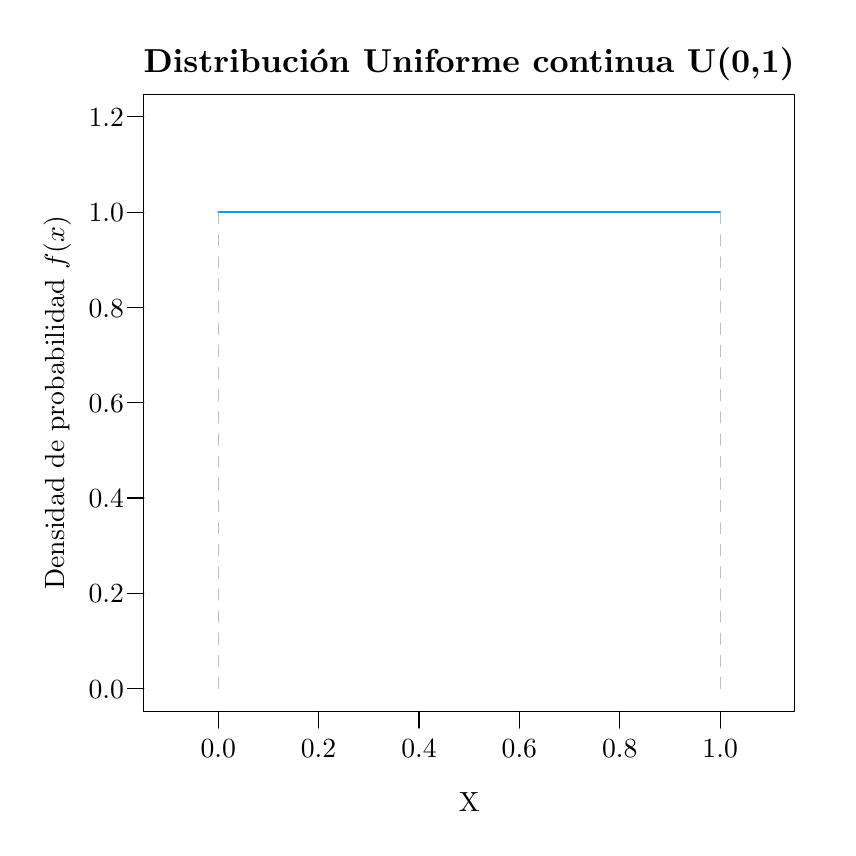
\begin{tikzpicture}[x=1pt,y=1pt]
\definecolor{fillColor}{RGB}{255,255,255}
\path[use as bounding box,fill=fillColor,fill opacity=0.00] (0,0) rectangle (289.08,289.08);
\begin{scope}
\path[clip] ( 42.00, 42.00) rectangle (277.08,265.08);
\definecolor{drawColor}{RGB}{5,161,230}

\path[draw=drawColor,line width= 0.8pt,line join=round,line cap=round] ( 68.85,222.39) --
	( 89.00,222.39) --
	(109.15,222.39) --
	(129.31,222.39) --
	(149.46,222.39) --
	(169.62,222.39) --
	(189.77,222.39) --
	(209.93,222.39) --
	(230.08,222.39) --
	(250.23,222.39);
\end{scope}
\begin{scope}
\path[clip] (  0.00,  0.00) rectangle (289.08,289.08);
\definecolor{drawColor}{RGB}{0,0,0}

\path[draw=drawColor,line width= 0.4pt,line join=round,line cap=round] ( 68.85, 42.00) -- (250.23, 42.00);

\path[draw=drawColor,line width= 0.4pt,line join=round,line cap=round] ( 68.85, 42.00) -- ( 68.85, 36.00);

\path[draw=drawColor,line width= 0.4pt,line join=round,line cap=round] (105.12, 42.00) -- (105.12, 36.00);

\path[draw=drawColor,line width= 0.4pt,line join=round,line cap=round] (141.40, 42.00) -- (141.40, 36.00);

\path[draw=drawColor,line width= 0.4pt,line join=round,line cap=round] (177.68, 42.00) -- (177.68, 36.00);

\path[draw=drawColor,line width= 0.4pt,line join=round,line cap=round] (213.96, 42.00) -- (213.96, 36.00);

\path[draw=drawColor,line width= 0.4pt,line join=round,line cap=round] (250.23, 42.00) -- (250.23, 36.00);

\node[text=drawColor,anchor=base,inner sep=0pt, outer sep=0pt, scale=  1.00] at ( 68.85, 25.20) {0.0};

\node[text=drawColor,anchor=base,inner sep=0pt, outer sep=0pt, scale=  1.00] at (105.12, 25.20) {0.2};

\node[text=drawColor,anchor=base,inner sep=0pt, outer sep=0pt, scale=  1.00] at (141.40, 25.20) {0.4};

\node[text=drawColor,anchor=base,inner sep=0pt, outer sep=0pt, scale=  1.00] at (177.68, 25.20) {0.6};

\node[text=drawColor,anchor=base,inner sep=0pt, outer sep=0pt, scale=  1.00] at (213.96, 25.20) {0.8};

\node[text=drawColor,anchor=base,inner sep=0pt, outer sep=0pt, scale=  1.00] at (250.23, 25.20) {1.0};

\path[draw=drawColor,line width= 0.4pt,line join=round,line cap=round] ( 42.00, 50.26) -- ( 42.00,256.82);

\path[draw=drawColor,line width= 0.4pt,line join=round,line cap=round] ( 42.00, 50.26) -- ( 36.00, 50.26);

\path[draw=drawColor,line width= 0.4pt,line join=round,line cap=round] ( 42.00, 84.69) -- ( 36.00, 84.69);

\path[draw=drawColor,line width= 0.4pt,line join=round,line cap=round] ( 42.00,119.11) -- ( 36.00,119.11);

\path[draw=drawColor,line width= 0.4pt,line join=round,line cap=round] ( 42.00,153.54) -- ( 36.00,153.54);

\path[draw=drawColor,line width= 0.4pt,line join=round,line cap=round] ( 42.00,187.97) -- ( 36.00,187.97);

\path[draw=drawColor,line width= 0.4pt,line join=round,line cap=round] ( 42.00,222.39) -- ( 36.00,222.39);

\path[draw=drawColor,line width= 0.4pt,line join=round,line cap=round] ( 42.00,256.82) -- ( 36.00,256.82);

\node[text=drawColor,anchor=base east,inner sep=0pt, outer sep=0pt, scale=  1.00] at ( 34.80, 46.82) {0.0};

\node[text=drawColor,anchor=base east,inner sep=0pt, outer sep=0pt, scale=  1.00] at ( 34.80, 81.24) {0.2};

\node[text=drawColor,anchor=base east,inner sep=0pt, outer sep=0pt, scale=  1.00] at ( 34.80,115.67) {0.4};

\node[text=drawColor,anchor=base east,inner sep=0pt, outer sep=0pt, scale=  1.00] at ( 34.80,150.10) {0.6};

\node[text=drawColor,anchor=base east,inner sep=0pt, outer sep=0pt, scale=  1.00] at ( 34.80,184.52) {0.8};

\node[text=drawColor,anchor=base east,inner sep=0pt, outer sep=0pt, scale=  1.00] at ( 34.80,218.95) {1.0};

\node[text=drawColor,anchor=base east,inner sep=0pt, outer sep=0pt, scale=  1.00] at ( 34.80,253.37) {1.2};

\path[draw=drawColor,line width= 0.4pt,line join=round,line cap=round] ( 42.00, 42.00) --
	(277.08, 42.00) --
	(277.08,265.08) --
	( 42.00,265.08) --
	( 42.00, 42.00);
\end{scope}
\begin{scope}
\path[clip] (  0.00,  0.00) rectangle (289.08,289.08);
\definecolor{drawColor}{RGB}{0,0,0}

\node[text=drawColor,anchor=base,inner sep=0pt, outer sep=0pt, scale=  1.20] at (159.54,272.89) {\bfseries Distribución Uniforme continua U(0,1)};

\node[text=drawColor,anchor=base,inner sep=0pt, outer sep=0pt, scale=  1.00] at (159.54,  6.00) {X};

\node[text=drawColor,rotate= 90.00,anchor=base,inner sep=0pt, outer sep=0pt, scale=  1.00] at ( 13.20,153.54) {Densidad de probabilidad $f(x)$};
\end{scope}
\begin{scope}
\path[clip] ( 42.00, 42.00) rectangle (277.08,265.08);
\definecolor{drawColor}{RGB}{190,190,190}

\path[draw=drawColor,line width= 0.4pt,dash pattern=on 4pt off 4pt ,line join=round,line cap=round] ( 68.85, 50.26) -- ( 68.85,222.39);

\path[draw=drawColor,line width= 0.4pt,dash pattern=on 4pt off 4pt ,line join=round,line cap=round] (250.23, 50.26) -- (250.23,222.39);
\end{scope}
\end{tikzpicture}
}
\end{center}

\note{
Un ejemplo de variable aleatoria uniforme continua sería la que mide el resultado de generar aleatoriamente un número entre 0 y 1. Esta
variable seguiría un modelo de distribución uniforme continuo $U(0,1)$, y la gráfica de su función de densidad es esta. Como se ve, la
función es constante y vale 1, ya que debe cumplirse, al ser función de densidad, que el área total por debajo de ella debe ser 1, y como en
realidad se trata del área de un rectángulo de base 1, pues la altura debe ser también 1.
}
\end{frame}


%---------------------------------------------------------------------slide----
\begin{frame}
\frametitle{Función de distribución de la Uniforme continua $U(a,b)$}
Como la función de densidad es constante, la función de distribución presenta un crecimiento lineal.
\begin{center}
\scalebox{0.7}{% Created by tikzDevice version 0.9 on 2016-04-28 17:47:04
% !TEX encoding = UTF-8 Unicode
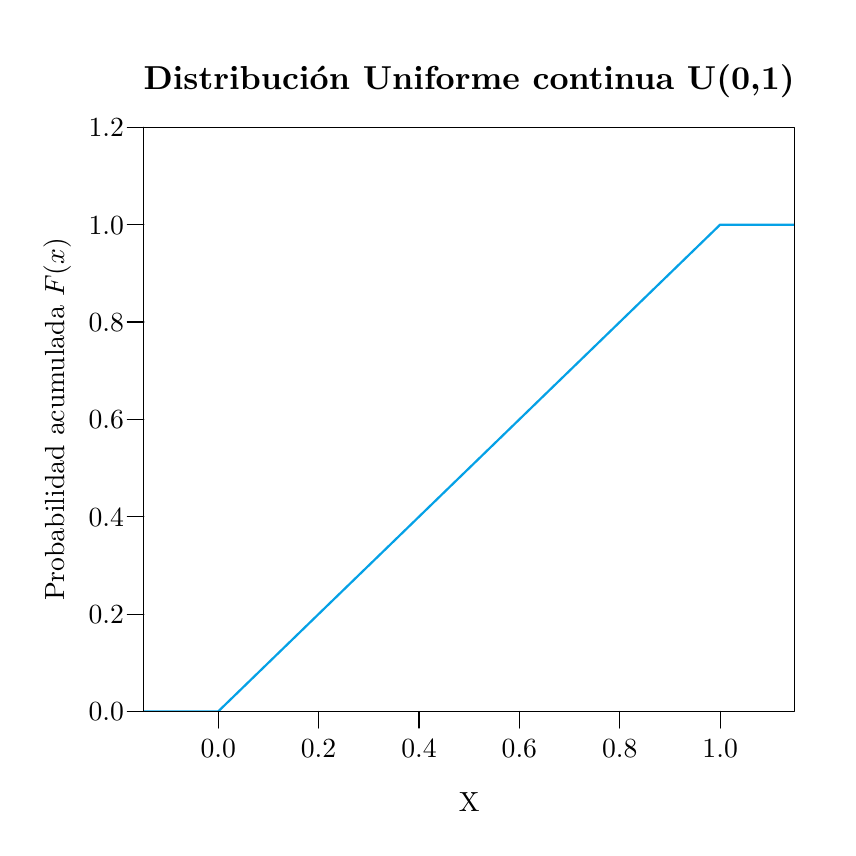
\begin{tikzpicture}[x=1pt,y=1pt]
\definecolor{fillColor}{RGB}{255,255,255}
\path[use as bounding box,fill=fillColor,fill opacity=0.00] (0,0) rectangle (289.08,289.08);
\begin{scope}
\path[clip] ( 42.00, 42.00) rectangle (277.08,253.08);
\definecolor{drawColor}{RGB}{5,161,230}

\path[draw=drawColor,line width= 0.8pt,line join=round,line cap=round] ( 32.57, 42.00) --
	( 68.85, 42.00) --
	( 89.00, 61.54) --
	(109.15, 81.09) --
	(129.31,100.63) --
	(149.46,120.18) --
	(169.62,139.72) --
	(189.77,159.27) --
	(209.93,178.81) --
	(230.08,198.36) --
	(250.23,217.90) --
	(286.51,217.90);
\end{scope}
\begin{scope}
\path[clip] (  0.00,  0.00) rectangle (289.08,289.08);
\definecolor{drawColor}{RGB}{0,0,0}

\path[draw=drawColor,line width= 0.4pt,line join=round,line cap=round] ( 68.85, 42.00) -- (250.23, 42.00);

\path[draw=drawColor,line width= 0.4pt,line join=round,line cap=round] ( 68.85, 42.00) -- ( 68.85, 36.00);

\path[draw=drawColor,line width= 0.4pt,line join=round,line cap=round] (105.12, 42.00) -- (105.12, 36.00);

\path[draw=drawColor,line width= 0.4pt,line join=round,line cap=round] (141.40, 42.00) -- (141.40, 36.00);

\path[draw=drawColor,line width= 0.4pt,line join=round,line cap=round] (177.68, 42.00) -- (177.68, 36.00);

\path[draw=drawColor,line width= 0.4pt,line join=round,line cap=round] (213.96, 42.00) -- (213.96, 36.00);

\path[draw=drawColor,line width= 0.4pt,line join=round,line cap=round] (250.23, 42.00) -- (250.23, 36.00);

\node[text=drawColor,anchor=base,inner sep=0pt, outer sep=0pt, scale=  1.00] at ( 68.85, 25.20) {0.0};

\node[text=drawColor,anchor=base,inner sep=0pt, outer sep=0pt, scale=  1.00] at (105.12, 25.20) {0.2};

\node[text=drawColor,anchor=base,inner sep=0pt, outer sep=0pt, scale=  1.00] at (141.40, 25.20) {0.4};

\node[text=drawColor,anchor=base,inner sep=0pt, outer sep=0pt, scale=  1.00] at (177.68, 25.20) {0.6};

\node[text=drawColor,anchor=base,inner sep=0pt, outer sep=0pt, scale=  1.00] at (213.96, 25.20) {0.8};

\node[text=drawColor,anchor=base,inner sep=0pt, outer sep=0pt, scale=  1.00] at (250.23, 25.20) {1.0};

\path[draw=drawColor,line width= 0.4pt,line join=round,line cap=round] ( 42.00, 42.00) -- ( 42.00,253.08);

\path[draw=drawColor,line width= 0.4pt,line join=round,line cap=round] ( 42.00, 42.00) -- ( 36.00, 42.00);

\path[draw=drawColor,line width= 0.4pt,line join=round,line cap=round] ( 42.00, 77.18) -- ( 36.00, 77.18);

\path[draw=drawColor,line width= 0.4pt,line join=round,line cap=round] ( 42.00,112.36) -- ( 36.00,112.36);

\path[draw=drawColor,line width= 0.4pt,line join=round,line cap=round] ( 42.00,147.54) -- ( 36.00,147.54);

\path[draw=drawColor,line width= 0.4pt,line join=round,line cap=round] ( 42.00,182.72) -- ( 36.00,182.72);

\path[draw=drawColor,line width= 0.4pt,line join=round,line cap=round] ( 42.00,217.90) -- ( 36.00,217.90);

\path[draw=drawColor,line width= 0.4pt,line join=round,line cap=round] ( 42.00,253.08) -- ( 36.00,253.08);

\node[text=drawColor,anchor=base east,inner sep=0pt, outer sep=0pt, scale=  1.00] at ( 34.80, 38.56) {0.0};

\node[text=drawColor,anchor=base east,inner sep=0pt, outer sep=0pt, scale=  1.00] at ( 34.80, 73.74) {0.2};

\node[text=drawColor,anchor=base east,inner sep=0pt, outer sep=0pt, scale=  1.00] at ( 34.80,108.92) {0.4};

\node[text=drawColor,anchor=base east,inner sep=0pt, outer sep=0pt, scale=  1.00] at ( 34.80,144.10) {0.6};

\node[text=drawColor,anchor=base east,inner sep=0pt, outer sep=0pt, scale=  1.00] at ( 34.80,179.28) {0.8};

\node[text=drawColor,anchor=base east,inner sep=0pt, outer sep=0pt, scale=  1.00] at ( 34.80,214.46) {1.0};

\node[text=drawColor,anchor=base east,inner sep=0pt, outer sep=0pt, scale=  1.00] at ( 34.80,249.64) {1.2};

\path[draw=drawColor,line width= 0.4pt,line join=round,line cap=round] ( 42.00, 42.00) --
	(277.08, 42.00) --
	(277.08,253.08) --
	( 42.00,253.08) --
	( 42.00, 42.00);
\end{scope}
\begin{scope}
\path[clip] (  0.00,  0.00) rectangle (289.08,289.08);
\definecolor{drawColor}{RGB}{0,0,0}

\node[text=drawColor,anchor=base,inner sep=0pt, outer sep=0pt, scale=  1.20] at (159.54,266.89) {\bfseries Distribución Uniforme continua U(0,1)};

\node[text=drawColor,anchor=base,inner sep=0pt, outer sep=0pt, scale=  1.00] at (159.54,  6.00) {X};

\node[text=drawColor,rotate= 90.00,anchor=base,inner sep=0pt, outer sep=0pt, scale=  1.00] at ( 13.20,147.54) {Probabilidad acumulada $F(x)$};
\end{scope}
\end{tikzpicture}
}
\end{center}

\note{
En esta otra gráfica tenemos la función de distribución $U(0,1)$.
Como la función de densidad es constante, la función de distribución presenta un crecimiento lineal. Obsérvese que, como para cualquier
función de distribución, la probabilidad acumulada al comienzo del recorrido es 0, y al final, vale 1, que es la probabilidad total. 
}
\end{frame}


% ---------------------------------------------------------------------slide----
\begin{frame}
\frametitle{Cálculo de probabilidades con una Uniforme continua}
\framesubtitle{Ejemplo de espera de un autobús}
Supóngase que un autobús pasa por una parada cada 15 minutos. Si una persona puede llegar a la parada en cualquier instante, \emph{¿cuál es
la probabilidad de que espere entre 5 y 10 minutos?}
\begin{columns}
\begin{column}{0.52\textwidth}
En este caso, la variable $X$ que mide el tiempo de espera sigue un modelo de distribución uniforme continua $U(0,15)$ ya que cualquier
valor entre los 0 y los 15 minutos es equipobrable.

Así pues, la probabilidad que nos piden es
\begin{align*}
P(5\leq X\leq 10) &= \int_{5}^{10} \frac{1}{15}\;dx = \left[\frac{x}{15}\right]_5^{10} = \\
&= \frac{10}{15}-\frac{5}{15} =\frac{1}{3}.
\end{align*}
\end{column}
\begin{column}{0.43\textwidth}
\begin{center}
\scalebox{0.5}{%% Input file name: calculo_probabilidades_uniforme.fig
%% FIG version: 3.2
%% Orientation: Landscape
%% Justification: Flush Left
%% Units: Inches
%% Paper size: A4
%% Magnification: 100.0
%% Resolution: 1200ppi
%% Include the following in the preamble:
%% \usepackage{textcomp}
%% End

\begin{pspicture}(6.68cm,3.48cm)(16.66cm,13.45cm)
\psset{unit=0.8cm}
%%
%% Depth: 2147483647
%%
\newgray{mycolor0}{0.74}\definecolor{mycolor0}{gray}{0.74}
\newrgbcolor{mycolor1}{1.00 0.50 0.31}\definecolor{mycolor1}{rgb}{1.00,0.50,0.31}
%%
%% Depth: 100
%%
\psset{linestyle=solid,linewidth=0.03175,linecolor=black,fillstyle=none}
\psline(10.90,13.59)(13.82,13.59)(16.73,13.59)(19.64,13.59)
\psset{fillstyle=solid,fillcolor=mycolor1}
\psline(13.82,6.80)(13.82,13.59)(16.73,13.59)(16.73,6.80)
\psset{fillstyle=none}
\psline(10.90,6.47)(19.64,6.47)
\psline(10.90,6.47)(10.90,6.26)
\psline(13.82,6.47)(13.82,6.26)
\psline(16.73,6.47)(16.73,6.26)
\psline(19.64,6.47)(19.64,6.26)
\rput(10.90,5.71){0}
\rput(13.82,5.71){5}
\rput(16.73,5.71){10}
\rput(19.64,5.71){15}
\psline(10.23,6.80)(10.23,14.95)
\psline(10.23,6.80)(10.02,6.80)
\psline(10.23,8.84)(10.02,8.84)
\psline(10.23,10.88)(10.02,10.88)
\psline(10.23,12.91)(10.02,12.91)
\psline(10.23,14.95)(10.02,14.95)
\rput{90}(9.73,6.80){0.00}
\rput{90}(9.73,8.84){0.02}
\rput{90}(9.73,10.88){0.04}
\rput{90}(9.73,12.91){0.06}
\rput{90}(9.73,14.95){0.08}
\psline(10.23,6.47)(20.31,6.47)(20.31,15.28)(10.23,15.28)(10.23,6.47)
\rput(15.27,15.99){Distribución Uniforme $U(0,15)$}
\rput(15.27,4.86){$X$}
\rput[l]{90}(8.86,9.54){Densidad $f(x)$}
\psset{linecolor=mycolor0}
\psline(10.23,6.80)(20.31,6.80)
\rput(15.27,10.78){$P(5\leq X\leq 10)=$}
\rput(15.27,9.76){$\int_5^{10}\frac{1}{15}\;dx$}
\psset{linestyle=dashed}
\psline(10.90,6.80)(10.90,13.59)
\psline(19.64,6.80)(19.64,13.59)
\end{pspicture}
%% End
}
\end{center}
\end{column}
\end{columns}
Además, el tiempo medio de espera será $\mu=\frac{0+15}{2}=7.5$ minutos.

\note{
Como ejemplo, supóngase que un autobús pasa por una parada cada 15 minutos. Si una persona puede llegar a la parada en cualquier instante,
\emph{¿cuál es la probabilidad de que espere entre 5 y 10 minutos?}

Está claro que lo mínimo que puede esperar una persona es 0 minutos, si llega justo cuando está el autobús, y lo máximo es 15 minutos, si
llega justo cuando el autobús se marcha. Como además puede llegar en cualquier instante con equiprobabiliadad, la variable $X$ que mide el
tiempo de espera sigue un modelo de distribución uniforme continua $U(0,15)$.

Así pues, la probabilidad que nos piden es
\begin{align*}
P(5\leq X\leq 10) &= \int_{5}^{10} \frac{1}{15}\;dx = \left[\frac{x}{15}\right]_5^{10} = \\
&= \frac{10}{15}-\frac{5}{15} =\frac{1}{3}.
\end{align*}

Aunque también podría calcularse fácilmente a partir de la gráfica de la función de densidad que es constante y vale $1/15$, midiendo el
área que queda por debajo de esta función entre 5 y 10. Como se tráta del área de un rectánculo, basta multiplicar la base, que es 5, por la
altura que es $1/15$ y de nuevo se obtiene $1/3$.
}
\end{frame}


\subsection{Distribución Normal}

%---------------------------------------------------------------------slide----
\begin{frame}
\frametitle{Distribución Normal $N(\mu,\sigma)$}
El modelo de distribución normal es, sin duda, el modelo de distribución continuo más importante, ya que es el que más a menudo se presenta
en la naturaleza.
\begin{definicion}[Distribución Normal]
Una variable aleatoria continua $X$ sigue un modelo de distribución \emph{normal} $N(\mu,\sigma)$ si su recorrido es $\mathbb{R}$ y su función de densidad vale
\[
f(x)= \frac{1}{\sigma\sqrt{2\pi}}e^{-\frac{(x-\mu)^2}{2\sigma^2}}.
\]
\end{definicion}

La distribución normal depende de dos parámetros $\mu$ y $\sigma$ que son, precisamente, su media y desviación típica.

\note{
El modelo de distribución normal es, sin duda, el modelo de distribución continuo más importante, ya que es el que más a menudo se presenta
en la naturaleza, sobre todo en variables continuas biológicas.

\begin{definicion}[Distribución Normal]
Una variable aleatoria continua $X$ sigue un modelo de distribución \emph{normal} $N(\mu,\sigma)$ si su recorrido es $\mathbb{R}$ y su función de densidad vale
\[
f(x)= \frac{1}{\sigma\sqrt{2\pi}}e^{-\frac{(x-\mu)^2}{2\sigma^2}}.
\]
\end{definicion}

La distribución normal depende de dos parámetros $\mu$ y $\sigma$ que son, precisamente, su media y desviación típica.
}
\end{frame}


%---------------------------------------------------------------------slide----
\begin{frame}
\frametitle{Función de densidad de la Normal $N(\mu,\sigma)$}
La gráfica de la función de densidad de la distribución normal tiene forma de una especie de campana, conocida como \emph{campana de Gauss}
(en honor a su descubridor), y está centrada en la media $\mu$.
\begin{center}
\scalebox{0.65}{% Created by tikzDevice version 0.10.1 on 2016-05-08 18:26:45
% !TEX encoding = UTF-8 Unicode
\begin{tikzpicture}[x=1pt,y=1pt]
\definecolor{fillColor}{RGB}{255,255,255}
\path[use as bounding box,fill=fillColor,fill opacity=0.00] (0,0) rectangle (289.08,289.08);
\begin{scope}
\path[clip] ( 42.00, 42.00) rectangle (277.08,253.08);
\definecolor{drawColor}{RGB}{5,161,230}

\path[draw=drawColor,line width= 0.8pt,line join=round,line cap=round] ( 50.71, 42.81) --
	( 52.36, 42.95) --
	( 54.00, 43.12) --
	( 55.65, 43.31) --
	( 57.30, 43.53) --
	( 58.95, 43.79) --
	( 60.60, 44.08) --
	( 62.25, 44.41) --
	( 63.90, 44.79) --
	( 65.55, 45.22) --
	( 67.20, 45.71) --
	( 68.85, 46.27) --
	( 70.49, 46.89) --
	( 72.14, 47.59) --
	( 73.79, 48.37) --
	( 75.44, 49.25) --
	( 77.09, 50.22) --
	( 78.74, 51.31) --
	( 80.39, 52.50) --
	( 82.04, 53.83) --
	( 83.69, 55.29) --
	( 85.34, 56.89) --
	( 86.98, 58.64) --
	( 88.63, 60.55) --
	( 90.28, 62.63) --
	( 91.93, 64.89) --
	( 93.58, 67.33) --
	( 95.23, 69.95) --
	( 96.88, 72.78) --
	( 98.53, 75.80) --
	(100.18, 79.03) --
	(101.83, 82.47) --
	(103.47, 86.12) --
	(105.12, 89.97) --
	(106.77, 94.03) --
	(108.42, 98.29) --
	(110.07,102.75) --
	(111.72,107.40) --
	(113.37,112.23) --
	(115.02,117.23) --
	(116.67,122.38) --
	(118.32,127.67) --
	(119.96,133.09) --
	(121.61,138.60) --
	(123.26,144.19) --
	(124.91,149.83) --
	(126.56,155.50) --
	(128.21,161.17) --
	(129.86,166.81) --
	(131.51,172.39) --
	(133.16,177.88) --
	(134.81,183.25) --
	(136.45,188.47) --
	(138.10,193.50) --
	(139.75,198.30) --
	(141.40,202.86) --
	(143.05,207.14) --
	(144.70,211.11) --
	(146.35,214.74) --
	(148.00,218.01) --
	(149.65,220.90) --
	(151.30,223.37) --
	(152.94,225.43) --
	(154.59,227.04) --
	(156.24,228.20) --
	(157.89,228.90) --
	(159.54,229.13) --
	(161.19,228.90) --
	(162.84,228.20) --
	(164.49,227.04) --
	(166.14,225.43) --
	(167.78,223.37) --
	(169.43,220.90) --
	(171.08,218.01) --
	(172.73,214.74) --
	(174.38,211.11) --
	(176.03,207.14) --
	(177.68,202.86) --
	(179.33,198.30) --
	(180.98,193.50) --
	(182.63,188.47) --
	(184.27,183.25) --
	(185.92,177.88) --
	(187.57,172.39) --
	(189.22,166.81) --
	(190.87,161.17) --
	(192.52,155.50) --
	(194.17,149.83) --
	(195.82,144.19) --
	(197.47,138.60) --
	(199.12,133.09) --
	(200.76,127.67) --
	(202.41,122.38) --
	(204.06,117.23) --
	(205.71,112.23) --
	(207.36,107.40) --
	(209.01,102.75) --
	(210.66, 98.29) --
	(212.31, 94.03) --
	(213.96, 89.97) --
	(215.61, 86.12) --
	(217.25, 82.47) --
	(218.90, 79.03) --
	(220.55, 75.80) --
	(222.20, 72.78) --
	(223.85, 69.95) --
	(225.50, 67.33) --
	(227.15, 64.89) --
	(228.80, 62.63) --
	(230.45, 60.55) --
	(232.10, 58.64) --
	(233.74, 56.89) --
	(235.39, 55.29) --
	(237.04, 53.83) --
	(238.69, 52.50) --
	(240.34, 51.31) --
	(241.99, 50.22) --
	(243.64, 49.25) --
	(245.29, 48.37) --
	(246.94, 47.59) --
	(248.59, 46.89) --
	(250.23, 46.27) --
	(251.88, 45.71) --
	(253.53, 45.22) --
	(255.18, 44.79) --
	(256.83, 44.41) --
	(258.48, 44.08) --
	(260.13, 43.79) --
	(261.78, 43.53) --
	(263.43, 43.31) --
	(265.08, 43.12) --
	(266.72, 42.95) --
	(268.37, 42.81);
\end{scope}
\begin{scope}
\path[clip] (  0.00,  0.00) rectangle (289.08,289.08);
\definecolor{drawColor}{RGB}{0,0,0}

\node[text=drawColor,anchor=base,inner sep=0pt, outer sep=0pt, scale=  1.20] at (159.54,266.89) {\bfseries Distribución Normal $N(\mu,\sigma)$};

\node[text=drawColor,anchor=base,inner sep=0pt, outer sep=0pt, scale=  1.00] at (159.54,  6.00) {X};

\node[text=drawColor,rotate= 90.00,anchor=base,inner sep=0pt, outer sep=0pt, scale=  1.00] at ( 13.20,147.54) {Densidad de probabilidad $f(x)$};
\end{scope}
\begin{scope}
\path[clip] (  0.00,  0.00) rectangle (289.08,289.08);
\definecolor{drawColor}{RGB}{0,0,0}

\path[draw=drawColor,line width= 0.4pt,line join=round,line cap=round] (159.54, 42.00) -- (159.54, 42.00);

\path[draw=drawColor,line width= 0.4pt,line join=round,line cap=round] (159.54, 42.00) -- (159.54, 36.00);

\node[text=drawColor,anchor=base,inner sep=0pt, outer sep=0pt, scale=  1.00] at (159.54, 25.20) {$\mu$};

\path[draw=drawColor,line width= 0.4pt,line join=round,line cap=round] ( 42.00, 42.00) --
	(277.08, 42.00) --
	(277.08,253.08) --
	( 42.00,253.08) --
	( 42.00, 42.00);
\end{scope}
\end{tikzpicture}
}
\end{center}

\note{
La gráfica de la función de densidad de la distribución normal tiene forma de una especie de campana, conocida como \emph{campana de Gauss}
(en honor a su descubridor), y está centrada en la media $\mu$.
}
\end{frame}


%---------------------------------------------------------------------slide----
\begin{frame}
\frametitle{Función de densidad de la Normal $N(\mu,\sigma)$}
La forma de la campana de Gauss depende de sus dos parámetros:
\begin{itemize}
\item La media $\mu$ determina dónde está centrada.
\item La desviación típica $\sigma$ determina su anchura.
\end{itemize} 
\begin{center}
\scalebox{0.5}{%% Input file name: funcion_densidad_normales_distinta_media.fig
%% FIG version: 3.2
%% Orientation: Landscape
%% Justification: Flush Left
%% Units: Inches
%% Paper size: A4
%% Magnification: 100.0
%% Resolution: 1200ppi

\begin{pspicture}(6.68cm,4.29cm)(16.66cm,13.45cm)
\psset{unit=0.8cm}
%%
%% Depth: 2147483647
%%
\newrgbcolor{mycolor0}{1.00 0.50 0.31}\definecolor{mycolor0}{rgb}{1.00,0.50,0.31}
\newrgbcolor{mycolor1}{0.28 0.46 1.00}\definecolor{mycolor1}{rgb}{0.28,0.46,1.00}
\newgray{mycolor2}{0.74}\definecolor{mycolor2}{gray}{0.74}
%%
%% Depth: 100
%%
\psset{linestyle=solid,linewidth=0.03175,linecolor=mycolor0,fillstyle=none}
\psline(10.62,7.82)(10.69,7.83)(10.76,7.84)(10.83,7.85)(10.91,7.87)(10.98,7.89)(11.05,7.91)(11.12,7.94)(11.20,7.97)(11.27,8.00)(11.34,8.04)(11.41,8.09)(11.48,8.15)(11.55,8.21)(11.63,8.29)(11.70,8.37)(11.77,8.47)(11.84,8.58)(11.92,8.70)(11.99,8.83)(12.06,8.98)(12.13,9.14)(12.20,9.32)(12.28,9.52)(12.35,9.73)(12.42,9.96)(12.49,10.20)(12.56,10.46)(12.64,10.73)(12.71,11.02)(12.78,11.32)(12.85,11.63)(12.93,11.95)(13.00,12.27)(13.07,12.60)(13.14,12.93)(13.21,13.26)(13.29,13.58)(13.36,13.90)(13.43,14.20)(13.50,14.49)(13.57,14.77)(13.65,15.02)(13.72,15.25)(13.79,15.45)(13.86,15.62)(13.94,15.76)(14.01,15.86)(14.08,15.94)(14.15,15.97)(14.22,15.97)(14.30,15.94)(14.37,15.86)(14.44,15.76)(14.51,15.62)(14.58,15.45)(14.66,15.25)(14.73,15.02)(14.80,14.77)(14.87,14.49)(14.95,14.20)(15.02,13.90)(15.09,13.58)(15.16,13.26)(15.23,12.93)(15.31,12.60)(15.38,12.27)(15.45,11.95)(15.52,11.63)(15.59,11.32)(15.67,11.02)(15.74,10.73)(15.81,10.46)(15.88,10.20)(15.96,9.96)(16.03,9.73)(16.10,9.52)(16.17,9.32)(16.24,9.14)(16.32,8.98)(16.39,8.83)(16.46,8.70)(16.53,8.58)(16.60,8.47)(16.68,8.37)(16.75,8.29)(16.82,8.21)(16.89,8.15)(16.97,8.09)(17.04,8.04)(17.11,8.00)(17.18,7.97)(17.25,7.94)(17.32,7.91)(17.40,7.89)(17.47,7.87)(17.54,7.85)(17.61,7.84)(17.68,7.83)(17.76,7.82)
\psset{linecolor=black}
\psline(12.02,7.49)(18.53,7.49)
\psline(12.02,7.49)(12.02,7.28)
\psline(14.19,7.49)(14.19,7.28)
\psline(16.36,7.49)(16.36,7.28)
\psline(18.53,7.49)(18.53,7.28)
\rput(12.02,6.73){-2}
\rput(14.19,6.73){0}
\rput(16.36,6.73){2}
\rput(18.53,6.73){4}
\psline(10.23,7.78)(10.23,16.00)
\psline(10.23,7.78)(10.02,7.78)
\psline(10.23,9.84)(10.02,9.84)
\psline(10.23,11.89)(10.02,11.89)
\psline(10.23,13.94)(10.02,13.94)
\psline(10.23,16.00)(10.02,16.00)
\rput{90}(9.73,7.78){0.0}
\rput{90}(9.73,9.84){0.1}
\rput{90}(9.73,11.89){0.2}
\rput{90}(9.73,13.94){0.3}
\rput{90}(9.73,16.00){0.4}
\psline(10.23,7.49)(20.31,7.49)(20.31,16.30)(10.23,16.30)(10.23,7.49)
\rput(15.27,5.88){$X$}
\rput[l]{90}(8.86,10.56){Densidad $f(x)$}
\psset{linecolor=mycolor1}
\psline(12.79,7.82)(12.86,7.83)(12.93,7.84)(13.00,7.85)(13.08,7.87)(13.15,7.89)(13.22,7.91)(13.29,7.94)(13.36,7.97)(13.44,8.00)(13.51,8.04)(13.58,8.09)(13.65,8.15)(13.72,8.21)(13.80,8.29)(13.87,8.37)(13.94,8.47)(14.01,8.58)(14.09,8.70)(14.16,8.83)(14.23,8.98)(14.30,9.14)(14.37,9.32)(14.45,9.52)(14.52,9.73)(14.59,9.96)(14.66,10.20)(14.73,10.46)(14.81,10.73)(14.88,11.02)(14.95,11.32)(15.02,11.63)(15.10,11.95)(15.17,12.27)(15.24,12.60)(15.31,12.93)(15.38,13.26)(15.46,13.58)(15.53,13.90)(15.60,14.20)(15.67,14.49)(15.74,14.77)(15.82,15.02)(15.89,15.25)(15.96,15.45)(16.03,15.62)(16.11,15.76)(16.18,15.86)(16.25,15.94)(16.32,15.97)(16.39,15.97)(16.47,15.94)(16.54,15.86)(16.61,15.76)(16.68,15.62)(16.75,15.45)(16.83,15.25)(16.90,15.02)(16.97,14.77)(17.04,14.49)(17.12,14.20)(17.19,13.90)(17.26,13.58)(17.33,13.26)(17.40,12.93)(17.48,12.60)(17.55,12.27)(17.62,11.95)(17.69,11.63)(17.76,11.32)(17.84,11.02)(17.91,10.73)(17.98,10.46)(18.05,10.20)(18.13,9.96)(18.20,9.73)(18.27,9.52)(18.34,9.32)(18.41,9.14)(18.48,8.98)(18.56,8.83)(18.63,8.70)(18.70,8.58)(18.77,8.47)(18.84,8.37)(18.92,8.29)(18.99,8.21)(19.06,8.15)(19.13,8.09)(19.21,8.04)(19.28,8.00)(19.35,7.97)(19.42,7.94)(19.49,7.91)(19.57,7.89)(19.64,7.87)(19.71,7.85)(19.78,7.84)(19.85,7.83)(19.93,7.82)
\psset{linecolor=mycolor2}
\psline(10.23,7.78)(20.31,7.78)
\psset{linecolor=mycolor0}
\psline(17.22,15.58)(17.85,15.58)
\psset{linecolor=mycolor1}
\psline(17.22,15.15)(17.85,15.15)
\rput[l](18.17,15.46){$N(0,1)$}
\rput[l](18.17,15.04){$N(2,1)$}
\end{pspicture}
%% End
}
\quad
\scalebox{0.5}{%% Input file name: funcion_densidad_normales_distinta_varianza.fig
%% FIG version: 3.2
%% Orientation: Landscape
%% Justification: Flush Left
%% Units: Inches
%% Paper size: A4
%% Magnification: 100.0
%% Resolution: 1200ppi

\begin{pspicture}(6.68cm,4.29cm)(16.66cm,13.45cm)
\psset{unit=0.8cm}
%%
%% Depth: 2147483647
%%
\newrgbcolor{mycolor0}{1.00 0.50 0.31}\definecolor{mycolor0}{rgb}{1.00,0.50,0.31}
\newrgbcolor{mycolor1}{0.28 0.46 1.00}\definecolor{mycolor1}{rgb}{0.28,0.46,1.00}
\newgray{mycolor2}{0.74}\definecolor{mycolor2}{gray}{0.74}
%%
%% Depth: 100
%%
\psset{linestyle=solid,linewidth=0.03175,linecolor=mycolor0,fillstyle=none}
\psline(12.95,7.82)(12.99,7.83)(13.04,7.84)(13.09,7.85)(13.13,7.87)(13.18,7.89)(13.23,7.91)(13.28,7.94)(13.32,7.97)(13.37,8.00)(13.42,8.04)(13.46,8.09)(13.51,8.15)(13.56,8.21)(13.60,8.29)(13.65,8.37)(13.70,8.47)(13.75,8.58)(13.79,8.70)(13.84,8.83)(13.89,8.98)(13.93,9.14)(13.98,9.32)(14.03,9.52)(14.07,9.73)(14.12,9.96)(14.17,10.20)(14.22,10.46)(14.26,10.73)(14.31,11.02)(14.36,11.32)(14.40,11.63)(14.45,11.95)(14.50,12.27)(14.54,12.60)(14.59,12.93)(14.64,13.26)(14.69,13.58)(14.73,13.90)(14.78,14.20)(14.83,14.49)(14.87,14.77)(14.92,15.02)(14.97,15.25)(15.01,15.45)(15.06,15.62)(15.11,15.76)(15.16,15.86)(15.20,15.94)(15.25,15.97)(15.30,15.97)(15.34,15.94)(15.39,15.86)(15.44,15.76)(15.48,15.62)(15.53,15.45)(15.58,15.25)(15.63,15.02)(15.67,14.77)(15.72,14.49)(15.76,14.20)(15.81,13.90)(15.86,13.58)(15.91,13.26)(15.95,12.93)(16.00,12.60)(16.05,12.27)(16.10,11.95)(16.14,11.63)(16.19,11.32)(16.23,11.02)(16.28,10.73)(16.33,10.46)(16.38,10.20)(16.42,9.96)(16.47,9.73)(16.52,9.52)(16.57,9.32)(16.61,9.14)(16.66,8.98)(16.70,8.83)(16.75,8.70)(16.80,8.58)(16.85,8.47)(16.89,8.37)(16.94,8.29)(16.99,8.21)(17.03,8.15)(17.08,8.09)(17.13,8.04)(17.17,8.00)(17.22,7.97)(17.27,7.94)(17.32,7.91)(17.36,7.89)(17.41,7.87)(17.46,7.85)(17.50,7.84)(17.55,7.83)(17.60,7.82)
\psset{linecolor=black}
\psline(11.03,7.49)(19.51,7.49)
\psline(11.03,7.49)(11.03,7.28)
\psline(12.45,7.49)(12.45,7.28)
\psline(13.86,7.49)(13.86,7.28)
\psline(15.27,7.49)(15.27,7.28)
\psline(16.69,7.49)(16.69,7.28)
\psline(18.10,7.49)(18.10,7.28)
\psline(19.51,7.49)(19.51,7.28)
\rput(11.03,6.73){-6}
\rput(12.45,6.73){-4}
\rput(13.86,6.73){-2}
\rput(15.27,6.73){0}
\rput(16.69,6.73){2}
\rput(18.10,6.73){4}
\rput(19.51,6.73){6}
\psline(10.23,7.78)(10.23,16.00)
\psline(10.23,7.78)(10.02,7.78)
\psline(10.23,9.84)(10.02,9.84)
\psline(10.23,11.89)(10.02,11.89)
\psline(10.23,13.94)(10.02,13.94)
\psline(10.23,16.00)(10.02,16.00)
\rput{90}(9.73,7.78){0.0}
\rput{90}(9.73,9.84){0.1}
\rput{90}(9.73,11.89){0.2}
\rput{90}(9.73,13.94){0.3}
\rput{90}(9.73,16.00){0.4}
\psline(10.23,7.49)(20.31,7.49)(20.31,16.30)(10.23,16.30)(10.23,7.49)
\rput(15.27,5.88){$X$}
\rput[l]{90}(8.86,10.56){Densidad $f(x)$}
\psset{linecolor=mycolor1}
\psline(10.62,7.80)(10.71,7.81)(10.81,7.81)(10.90,7.82)(11.00,7.83)(11.09,7.83)(11.18,7.85)(11.28,7.86)(11.37,7.87)(11.47,7.89)(11.56,7.91)(11.65,7.94)(11.75,7.97)(11.84,8.00)(11.94,8.04)(12.03,8.08)(12.12,8.13)(12.22,8.18)(12.31,8.24)(12.41,8.31)(12.50,8.38)(12.59,8.46)(12.69,8.55)(12.78,8.65)(12.88,8.76)(12.97,8.87)(13.06,8.99)(13.16,9.12)(13.25,9.26)(13.35,9.40)(13.44,9.55)(13.53,9.71)(13.63,9.87)(13.72,10.03)(13.82,10.19)(13.91,10.36)(14.00,10.52)(14.10,10.68)(14.19,10.84)(14.29,10.99)(14.38,11.14)(14.47,11.28)(14.57,11.40)(14.66,11.51)(14.76,11.62)(14.85,11.70)(14.94,11.77)(15.04,11.82)(15.13,11.86)(15.23,11.88)(15.32,11.88)(15.41,11.86)(15.51,11.82)(15.60,11.77)(15.70,11.70)(15.79,11.62)(15.88,11.51)(15.98,11.40)(16.07,11.28)(16.16,11.14)(16.26,10.99)(16.35,10.84)(16.45,10.68)(16.54,10.52)(16.63,10.36)(16.73,10.19)(16.82,10.03)(16.92,9.87)(17.01,9.71)(17.10,9.55)(17.20,9.40)(17.29,9.26)(17.39,9.12)(17.48,8.99)(17.57,8.87)(17.67,8.76)(17.76,8.65)(17.86,8.55)(17.95,8.46)(18.04,8.38)(18.14,8.31)(18.23,8.24)(18.33,8.18)(18.42,8.13)(18.51,8.08)(18.61,8.04)(18.70,8.00)(18.80,7.97)(18.89,7.94)(18.98,7.91)(19.08,7.89)(19.17,7.87)(19.27,7.86)(19.36,7.85)(19.45,7.83)(19.55,7.83)(19.64,7.82)(19.74,7.81)(19.83,7.81)(19.92,7.80)
\psset{linecolor=mycolor2}
\psline(10.23,7.78)(20.31,7.78)
\psset{linecolor=mycolor0}
\psline(17.14,15.58)(17.78,15.58)
\psset{linecolor=mycolor1}
\psline(17.14,15.15)(17.78,15.15)
\rput[l](18.10,15.46){$N(0,1)$}
\rput[l](18.10,15.04){$N(0,2)$}
\end{pspicture}
%% End
}
\end{center}

\note{
La forma de la campana de Gauss depende de sus dos parámetros:
\begin{itemize}
\item Por un lado, ya hemos visto que la media $\mu$ determina dónde está centrada. En la gráfica de la izquierda podemos ver las funciones
de densidad de dos normales, una con media 0 y desviación típica 1, y otra con media 2 y desviación típica 1. Como se ve, ambas gráficas son
idénticas, salvo que la primera está centrada en el 0 y la segunda en el 2.
\item Por otro lado, la desviación típica $\sigma$, al ser una medida de la dispersión de la población, determina su anchura. En la gráfica
de la derecha podemos ver las funciones de densidad de dos normales con la misma media 0, y desviaciones típicas 1, y 2 respectivamente.
Como se ve, ambas están centradas en el 0, pero la primera es más estrecha que la segunda al tener menos dispersión. 
\end{itemize} 
}
\end{frame}


%---------------------------------------------------------------------slide----
\begin{frame}
\frametitle{Función de distribución de la Normal $N(\mu,\sigma)$}
Por su parte, la gráfica de la función de distribución tiene forma de S. 
\begin{center}
\scalebox{0.7}{%% Input file name: funcion_distribucion_normal_estandar.fig
%% FIG version: 3.2
%% Orientation: Landscape
%% Justification: Flush Left
%% Units: Inches
%% Paper size: A4
%% Magnification: 100.0
%% Resolution: 1200ppi
%% Include the following in the preamble:
%% \usepackage{textcomp}
%% End

\begin{pspicture}(6.69cm,3.44cm)(16.66cm,13.45cm)
\psset{unit=0.8cm}
%%
%% Depth: 2147483647
%%
\newgray{mycolor0}{0.74}\definecolor{mycolor0}{gray}{0.74}
\newrgbcolor{mycolor1}{1.00 0.50 0.31}\definecolor{mycolor1}{rgb}{1.00,0.50,0.31}
%%
%% Depth: 100
%%
\psset{linestyle=solid,linewidth=0.03175,linecolor=mycolor1,fillstyle=none}
\psline(10.61,6.75)(10.70,6.76)(10.80,6.76)(10.89,6.76)(10.99,6.76)(11.08,6.76)(11.17,6.77)(11.27,6.77)(11.36,6.78)(11.46,6.78)(11.55,6.79)(11.64,6.79)(11.74,6.80)(11.83,6.81)(11.93,6.83)(12.02,6.84)(12.12,6.86)(12.21,6.88)(12.30,6.90)(12.40,6.92)(12.49,6.95)(12.59,6.99)(12.68,7.03)(12.78,7.07)(12.87,7.12)(12.96,7.17)(13.06,7.23)(13.15,7.30)(13.25,7.37)(13.34,7.46)(13.43,7.55)(13.53,7.64)(13.62,7.75)(13.72,7.86)(13.81,7.99)(13.91,8.12)(14.00,8.26)(14.09,8.41)(14.19,8.56)(14.28,8.73)(14.38,8.90)(14.47,9.08)(14.56,9.27)(14.66,9.47)(14.76,9.67)(14.85,9.87)(14.94,10.08)(15.04,10.29)(15.13,10.51)(15.23,10.72)(15.32,10.94)(15.41,11.15)(15.51,11.37)(15.60,11.58)(15.70,11.79)(15.79,12.00)(15.89,12.20)(15.98,12.39)(16.07,12.58)(16.17,12.76)(16.26,12.93)(16.36,13.10)(16.45,13.26)(16.54,13.40)(16.64,13.54)(16.73,13.68)(16.83,13.80)(16.92,13.91)(17.02,14.02)(17.11,14.12)(17.20,14.21)(17.30,14.29)(17.39,14.36)(17.49,14.43)(17.58,14.49)(17.68,14.55)(17.77,14.59)(17.86,14.64)(17.96,14.67)(18.05,14.71)(18.15,14.74)(18.24,14.76)(18.33,14.79)(18.43,14.81)(18.52,14.82)(18.62,14.84)(18.71,14.85)(18.81,14.86)(18.90,14.87)(18.99,14.88)(19.09,14.88)(19.18,14.89)(19.28,14.89)(19.37,14.90)(19.47,14.90)(19.56,14.90)(19.66,14.90)(19.75,14.91)(19.84,14.91)(19.94,14.91)
\psset{linecolor=black}
\psline(11.02,6.43)(19.52,6.43)
\psline(15.27,6.43)(15.27,6.22)
\rput(15.27,5.67){$\mu$}
\psline(10.23,6.75)(10.23,14.91)
\psline(10.23,6.75)(10.02,6.75)
\psline(10.23,8.38)(10.02,8.38)
\psline(10.23,10.02)(10.02,10.02)
\psline(10.23,11.65)(10.02,11.65)
\psline(10.23,13.28)(10.02,13.28)
\psline(10.23,14.91)(10.02,14.91)
\rput{90}(9.73,6.75){0.0}
\rput{90}(9.73,8.38){0.2}
\rput{90}(9.73,10.02){0.4}
\rput{90}(9.73,11.65){0.6}
\rput{90}(9.73,13.28){0.8}
\rput{90}(9.73,14.91){1.0}
\psline(10.23,6.43)(20.31,6.43)(20.31,15.23)(10.23,15.23)(10.23,6.43)
\rput[l](12.14,15.99){Distribución normal $N(\mu,\sigma)$}
\rput(15.27,4.82){$X$}
\rput[l]{90}(8.88,8.51){Probabilidad acumulada $F(x)$}
\psset{linecolor=mycolor0}
\psline(10.23,6.75)(20.31,6.75)
\end{pspicture}
%% End
}
\end{center}

\note{
Por su parte, la gráfica de la función de distribución de una normal siempre tiene forma de S. 
}
\end{frame}


%---------------------------------------------------------------------slide----
\begin{frame}
\frametitle{Propiedades de la distribución Normal}
\begin{itemize}
\item La función de densidad es simétrica respecto a la media y por tanto, su coeficiente de asimetría es $g_1=0$.
\item También es mesocúrtica, y por tanto, su coeficiente de apuntamiento vale $g_2=0$.
\item La media, la mediana y la moda coinciden
\[
\mu = Me = Mo.
\]
\item Tiende asintóticamente a 0 cuando $x$ tiende a $\pm \infty$.
\end{itemize}

\note{
La distribución normal tiene propiedades muy interesantes:
\begin{itemize}
\item La función de densidad es simétrica respecto a la media y por tanto, su coeficiente de asimetría es $g_1=0$.
\item También es mesocúrtica, y por tanto, su coeficiente de apuntamiento vale $g_2=0$. Recordemos que el apuntamiento de cualquier variable
se compara precisamente con el apuntamiento de la distribución normal, ya que al ser esta la distribución más común, se toma como
referencia.
\item De nuevo, al ser simétrica con respecto a la media, hasta la media tendremos acumulada la mitad de la probabilidad, y por tanto la
media coincide con la mediana, y también con la moda, ya que sobre la media se alcanza el máximo de la función de densidad.
\[
\mu = Me = Mo.
\]
\item Tiende asintóticamente a 0 cuando $x$ tiende a $\pm \infty$.
\end{itemize}
}
\end{frame}


%---------------------------------------------------------------------slide----
\begin{frame}
\frametitle{Propiedades de la distribución Normal}
\begin{itemize}
\item Se cumple que
\begin{align*}
& P(\mu-\sigma \leq X \leq \mu+\sigma) = 0.68,\\
& P(\mu-2\sigma \leq X \leq \mu+2\sigma) = 0.95,\\
& P(\mu-3\sigma \leq X \leq \mu+3\sigma) = 0.99.
\end{align*}
\end{itemize}
\begin{center}
\scalebox{0.6}{%% Input file name: variables_aleatorias_continuas/propiedades_normal_1.fig
%% FIG version: 3.2
%% Orientation: Landscape
%% Justification: Flush Left
%% Units: Inches
%% Paper size: A4
%% Magnification: 100.0
%% Resolution: 1200ppi
%% Include the following in the preamble:
%% \usepackage{textcomp}
%% End

\begin{pspicture}(6.68cm,3.44cm)(16.66cm,13.45cm)
\psset{unit=0.8cm}
%%
%% Depth: 2147483647
%%
\newrgbcolor{mycolor0}{1.00 0.50 0.31}\definecolor{mycolor0}{rgb}{1.00,0.50,0.31}
\newgray{mycolor1}{0.74}\definecolor{mycolor1}{gray}{0.74}
%%
%% Depth: 100
%%
\psset{linestyle=solid,linewidth=0.03175,linecolor=black}
\psline(11.03,6.43)(19.51,6.43)
\psline(11.03,6.43)(11.03,6.22)
\psline(12.45,6.43)(12.45,6.22)
\psline(13.86,6.43)(13.86,6.22)
\psline(15.27,6.43)(15.27,6.22)
\psline(16.69,6.43)(16.69,6.22)
\psline(18.10,6.43)(18.10,6.22)
\psline(19.51,6.43)(19.51,6.22)
\rput(15.27,5.67){$\mu$}
\psline(10.23,6.43)(20.31,6.43)(20.31,15.23)(10.23,15.23)(10.23,6.43)
\rput(15.27,15.99){Distribución normal $N(\mu,\sigma)$}
\rput(15.27,4.82){$X$}
\rput[l]{90}(9.50,9.50){Densidad $f(x)$}
\psline(10.61,6.75)(10.68,6.76)(10.75,6.77)(10.82,6.78)(10.89,6.79)(10.96,6.80)(11.03,6.81)(11.10,6.82)(11.17,6.84)(11.24,6.86)(11.32,6.88)(11.39,6.91)(11.46,6.93)(11.53,6.96)(11.60,7.00)(11.67,7.04)(11.74,7.08)(11.81,7.13)(11.88,7.18)(11.95,7.24)(12.02,7.30)(12.09,7.37)(12.16,7.45)(12.23,7.53)(12.30,7.62)(12.37,7.72)(12.45,7.83)(12.52,7.94)(12.59,8.07)(12.66,8.20)(12.73,8.34)(12.80,8.49)(12.87,8.65)(12.94,8.82)(13.01,9.00)(13.08,9.18)(13.15,9.38)(13.22,9.58)(13.29,9.79)(13.36,10.01)(13.43,10.24)(13.51,10.47)(13.58,10.71)(13.65,10.95)(13.72,11.19)(13.79,11.44)(13.86,11.69)(13.93,11.93)(14.00,12.18)(14.07,12.42)(14.14,12.67)(14.21,12.90)(14.28,13.13)(14.35,13.35)(14.43,13.56)(14.49,13.76)(14.56,13.95)(14.64,14.12)(14.71,14.28)(14.78,14.42)(14.85,14.55)(14.92,14.66)(14.99,14.75)(15.06,14.82)(15.13,14.87)(15.20,14.90)(15.27,14.91)(15.34,14.90)(15.41,14.87)(15.49,14.82)(15.56,14.75)(15.63,14.66)(15.70,14.55)(15.77,14.42)(15.84,14.28)(15.91,14.12)(15.98,13.95)(16.05,13.76)(16.12,13.56)(16.19,13.35)(16.26,13.13)(16.33,12.90)(16.40,12.67)(16.47,12.42)(16.54,12.18)(16.62,11.93)(16.69,11.69)(16.76,11.44)(16.83,11.19)(16.90,10.95)(16.97,10.71)(17.04,10.47)(17.11,10.24)(17.18,10.01)(17.25,9.79)(17.32,9.58)(17.39,9.38)(17.46,9.18)(17.53,9.00)(17.60,8.82)(17.68,8.65)(17.75,8.49)(17.82,8.34)(17.89,8.20)(17.96,8.07)(18.03,7.94)(18.10,7.83)(18.17,7.72)(18.24,7.62)(18.31,7.53)(18.38,7.45)(18.45,7.37)(18.52,7.30)(18.59,7.24)(18.66,7.18)(18.74,7.13)(18.81,7.08)(18.88,7.04)(18.95,7.00)(19.02,6.96)(19.09,6.93)(19.16,6.91)(19.23,6.88)(19.30,6.86)(19.37,6.84)(19.44,6.82)(19.51,6.81)(19.58,6.80)(19.66,6.79)(19.73,6.78)(19.80,6.77)(19.87,6.76)(19.94,6.75)
\psset{linecolor=mycolor1}
\psline(10.23,6.72)(20.31,6.72)
\uncover<2>{
\psset{linecolor=mycolor1,fillstyle=solid,fillcolor=mycolor0}
\psline(13.86,6.72)(13.86,11.69)(13.93,11.93)(14.00,12.18)(14.07,12.42)(14.14,12.67)(14.21,12.90)(14.28,13.13)(14.35,13.35)(14.43,13.56)(14.49,13.76)(14.56,13.95)(14.64,14.12)(14.71,14.28)(14.78,14.42)(14.85,14.55)(14.92,14.66)(14.99,14.75)(15.06,14.82)(15.13,14.87)(15.20,14.90)(15.27,14.91)(15.34,14.90)(15.41,14.87)(15.49,14.82)(15.56,14.75)(15.63,14.66)(15.70,14.55)(15.77,14.42)(15.84,14.28)(15.91,14.12)(15.98,13.95)(16.05,13.76)(16.12,13.56)(16.19,13.35)(16.26,13.13)(16.33,12.90)(16.40,12.67)(16.47,12.42)(16.54,12.18)(16.62,11.93)(16.69,11.69)(16.69,6.72)
\psset{linecolor=black,fillstyle=none}
\psline(10.61,6.75)(10.68,6.76)(10.75,6.77)(10.82,6.78)(10.89,6.79)(10.96,6.80)(11.03,6.81)(11.10,6.82)(11.17,6.84)(11.24,6.86)(11.32,6.88)(11.39,6.91)(11.46,6.93)(11.53,6.96)(11.60,7.00)(11.67,7.04)(11.74,7.08)(11.81,7.13)(11.88,7.18)(11.95,7.24)(12.02,7.30)(12.09,7.37)(12.16,7.45)(12.23,7.53)(12.30,7.62)(12.37,7.72)(12.45,7.83)(12.52,7.94)(12.59,8.07)(12.66,8.20)(12.73,8.34)(12.80,8.49)(12.87,8.65)(12.94,8.82)(13.01,9.00)(13.08,9.18)(13.15,9.38)(13.22,9.58)(13.29,9.79)(13.36,10.01)(13.43,10.24)(13.51,10.47)(13.58,10.71)(13.65,10.95)(13.72,11.19)(13.79,11.44)(13.86,11.69)(13.93,11.93)(14.00,12.18)(14.07,12.42)(14.14,12.67)(14.21,12.90)(14.28,13.13)(14.35,13.35)(14.43,13.56)(14.49,13.76)(14.56,13.95)(14.64,14.12)(14.71,14.28)(14.78,14.42)(14.85,14.55)(14.92,14.66)(14.99,14.75)(15.06,14.82)(15.13,14.87)(15.20,14.90)(15.27,14.91)(15.34,14.90)(15.41,14.87)(15.49,14.82)(15.56,14.75)(15.63,14.66)(15.70,14.55)(15.77,14.42)(15.84,14.28)(15.91,14.12)(15.98,13.95)(16.05,13.76)(16.12,13.56)(16.19,13.35)(16.26,13.13)(16.33,12.90)(16.40,12.67)(16.47,12.42)(16.54,12.18)(16.62,11.93)(16.69,11.69)(16.76,11.44)(16.83,11.19)(16.90,10.95)(16.97,10.71)(17.04,10.47)(17.11,10.24)(17.18,10.01)(17.25,9.79)(17.32,9.58)(17.39,9.38)(17.46,9.18)(17.53,9.00)(17.60,8.82)(17.68,8.65)(17.75,8.49)(17.82,8.34)(17.89,8.20)(17.96,8.07)(18.03,7.94)(18.10,7.83)(18.17,7.72)(18.24,7.62)(18.31,7.53)(18.38,7.45)(18.45,7.37)(18.52,7.30)(18.59,7.24)(18.66,7.18)(18.74,7.13)(18.81,7.08)(18.88,7.04)(18.95,7.00)(19.02,6.96)(19.09,6.93)(19.16,6.91)(19.23,6.88)(19.30,6.86)(19.37,6.84)(19.44,6.82)(19.51,6.81)(19.58,6.80)(19.66,6.79)(19.73,6.78)(19.80,6.77)(19.87,6.76)(19.94,6.75)
\rput(13.86,5.67){$\mu-\sigma$}
\rput(16.69,5.67){$\mu+\sigma$}
\rput[B](15.27,7.62){68\%}
}
\uncover<3>{
\psset{linecolor=mycolor1,fillstyle=solid,fillcolor=mycolor0}
\psline(12.45,6.72)(12.45,7.83)(12.52,7.94)(12.59,8.07)(12.66,8.20)(12.73,8.34)(12.80,8.49)(12.87,8.65)(12.94,8.82)(13.01,9.00)(13.08,9.18)(13.15,9.38)(13.22,9.58)(13.29,9.79)(13.36,10.01)(13.43,10.24)(13.51,10.47)(13.58,10.71)(13.65,10.95)(13.72,11.19)(13.79,11.44)(13.86,11.69)(13.93,11.93)(14.00,12.18)(14.07,12.42)(14.14,12.67)(14.21,12.90)(14.28,13.13)(14.35,13.35)(14.43,13.56)(14.49,13.76)(14.56,13.95)(14.64,14.12)(14.71,14.28)(14.78,14.42)(14.85,14.55)(14.92,14.66)(14.99,14.75)(15.06,14.82)(15.13,14.87)(15.20,14.90)(15.27,14.91)(15.34,14.90)(15.41,14.87)(15.49,14.82)(15.56,14.75)(15.63,14.66)(15.70,14.55)(15.77,14.42)(15.84,14.28)(15.91,14.12)(15.98,13.95)(16.05,13.76)(16.12,13.56)(16.19,13.35)(16.26,13.13)(16.33,12.90)(16.40,12.67)(16.47,12.42)(16.54,12.18)(16.62,11.93)(16.69,11.69)(16.76,11.44)(16.83,11.19)(16.90,10.95)(16.97,10.71)(17.04,10.47)(17.11,10.24)(17.18,10.01)(17.25,9.79)(17.32,9.58)(17.39,9.38)(17.46,9.18)(17.53,9.00)(17.60,8.82)(17.68,8.65)(17.75,8.49)(17.82,8.34)(17.89,8.20)(17.96,8.07)(18.03,7.94)(18.10,7.83)(18.10,6.72)
\psset{linecolor=black,fillstyle=none}
\psline(10.61,6.75)(10.68,6.76)(10.75,6.77)(10.82,6.78)(10.89,6.79)(10.96,6.80)(11.03,6.81)(11.10,6.82)(11.17,6.84)(11.24,6.86)(11.32,6.88)(11.39,6.91)(11.46,6.93)(11.53,6.96)(11.60,7.00)(11.67,7.04)(11.74,7.08)(11.81,7.13)(11.88,7.18)(11.95,7.24)(12.02,7.30)(12.09,7.37)(12.16,7.45)(12.23,7.53)(12.30,7.62)(12.37,7.72)(12.45,7.83)(12.52,7.94)(12.59,8.07)(12.66,8.20)(12.73,8.34)(12.80,8.49)(12.87,8.65)(12.94,8.82)(13.01,9.00)(13.08,9.18)(13.15,9.38)(13.22,9.58)(13.29,9.79)(13.36,10.01)(13.43,10.24)(13.51,10.47)(13.58,10.71)(13.65,10.95)(13.72,11.19)(13.79,11.44)(13.86,11.69)(13.93,11.93)(14.00,12.18)(14.07,12.42)(14.14,12.67)(14.21,12.90)(14.28,13.13)(14.35,13.35)(14.43,13.56)(14.49,13.76)(14.56,13.95)(14.64,14.12)(14.71,14.28)(14.78,14.42)(14.85,14.55)(14.92,14.66)(14.99,14.75)(15.06,14.82)(15.13,14.87)(15.20,14.90)(15.27,14.91)(15.34,14.90)(15.41,14.87)(15.49,14.82)(15.56,14.75)(15.63,14.66)(15.70,14.55)(15.77,14.42)(15.84,14.28)(15.91,14.12)(15.98,13.95)(16.05,13.76)(16.12,13.56)(16.19,13.35)(16.26,13.13)(16.33,12.90)(16.40,12.67)(16.47,12.42)(16.54,12.18)(16.62,11.93)(16.69,11.69)(16.76,11.44)(16.83,11.19)(16.90,10.95)(16.97,10.71)(17.04,10.47)(17.11,10.24)(17.18,10.01)(17.25,9.79)(17.32,9.58)(17.39,9.38)(17.46,9.18)(17.53,9.00)(17.60,8.82)(17.68,8.65)(17.75,8.49)(17.82,8.34)(17.89,8.20)(17.96,8.07)(18.03,7.94)(18.10,7.83)(18.17,7.72)(18.24,7.62)(18.31,7.53)(18.38,7.45)(18.45,7.37)(18.52,7.30)(18.59,7.24)(18.66,7.18)(18.74,7.13)(18.81,7.08)(18.88,7.04)(18.95,7.00)(19.02,6.96)(19.09,6.93)(19.16,6.91)(19.23,6.88)(19.30,6.86)(19.37,6.84)(19.44,6.82)(19.51,6.81)(19.58,6.80)(19.66,6.79)(19.73,6.78)(19.80,6.77)(19.87,6.76)(19.94,6.75)
\rput(12.45,5.67){$\mu-2\sigma$}
\rput(18.10,5.67){$\mu+2\sigma$}
\rput[B](15.27,7.62){95\%}
}
\uncover<4>{
\psset{linecolor=mycolor1,fillstyle=solid,fillcolor=mycolor0}
\psline(11.03,6.72)(11.03,6.81)(11.10,6.82)(11.17,6.84)(11.24,6.86)(11.32,6.88)(11.39,6.91)(11.46,6.93)(11.53,6.96)(11.60,7.00)(11.67,7.04)(11.74,7.08)(11.81,7.13)(11.88,7.18)(11.95,7.24)(12.02,7.30)(12.09,7.37)(12.16,7.45)(12.23,7.53)(12.30,7.62)(12.37,7.72)(12.45,7.83)(12.52,7.94)(12.59,8.07)(12.66,8.20)(12.73,8.34)(12.80,8.49)(12.87,8.65)(12.94,8.82)(13.01,9.00)(13.08,9.18)(13.15,9.38)(13.22,9.58)(13.29,9.79)(13.36,10.01)(13.43,10.24)(13.51,10.47)(13.58,10.71)(13.65,10.95)(13.72,11.19)(13.79,11.44)(13.86,11.69)(13.93,11.93)(14.00,12.18)(14.07,12.42)(14.14,12.67)(14.21,12.90)(14.28,13.13)(14.35,13.35)(14.43,13.56)(14.49,13.76)(14.56,13.95)(14.64,14.12)(14.71,14.28)(14.78,14.42)(14.85,14.55)(14.92,14.66)(14.99,14.75)(15.06,14.82)(15.13,14.87)(15.20,14.90)(15.27,14.91)(15.34,14.90)(15.41,14.87)(15.49,14.82)(15.56,14.75)(15.63,14.66)(15.70,14.55)(15.77,14.42)(15.84,14.28)(15.91,14.12)(15.98,13.95)(16.05,13.76)(16.12,13.56)(16.19,13.35)(16.26,13.13)(16.33,12.90)(16.40,12.67)(16.47,12.42)(16.54,12.18)(16.62,11.93)(16.69,11.69)(16.76,11.44)(16.83,11.19)(16.90,10.95)(16.97,10.71)(17.04,10.47)(17.11,10.24)(17.18,10.01)(17.25,9.79)(17.32,9.58)(17.39,9.38)(17.46,9.18)(17.53,9.00)(17.60,8.82)(17.68,8.65)(17.75,8.49)(17.82,8.34)(17.89,8.20)(17.96,8.07)(18.03,7.94)(18.10,7.83)(18.17,7.72)(18.24,7.62)(18.31,7.53)(18.38,7.45)(18.45,7.37)(18.52,7.30)(18.59,7.24)(18.66,7.18)(18.74,7.13)(18.81,7.08)(18.88,7.04)(18.95,7.00)(19.02,6.96)(19.09,6.93)(19.16,6.91)(19.23,6.88)(19.30,6.86)(19.37,6.84)(19.44,6.82)(19.51,6.81)(19.51,6.72)
\psset{linecolor=black,fillstyle=none}
\psline(10.61,6.75)(10.68,6.76)(10.75,6.77)(10.82,6.78)(10.89,6.79)(10.96,6.80)(11.03,6.81)(11.10,6.82)(11.17,6.84)(11.24,6.86)(11.32,6.88)(11.39,6.91)(11.46,6.93)(11.53,6.96)(11.60,7.00)(11.67,7.04)(11.74,7.08)(11.81,7.13)(11.88,7.18)(11.95,7.24)(12.02,7.30)(12.09,7.37)(12.16,7.45)(12.23,7.53)(12.30,7.62)(12.37,7.72)(12.45,7.83)(12.52,7.94)(12.59,8.07)(12.66,8.20)(12.73,8.34)(12.80,8.49)(12.87,8.65)(12.94,8.82)(13.01,9.00)(13.08,9.18)(13.15,9.38)(13.22,9.58)(13.29,9.79)(13.36,10.01)(13.43,10.24)(13.51,10.47)(13.58,10.71)(13.65,10.95)(13.72,11.19)(13.79,11.44)(13.86,11.69)(13.93,11.93)(14.00,12.18)(14.07,12.42)(14.14,12.67)(14.21,12.90)(14.28,13.13)(14.35,13.35)(14.43,13.56)(14.49,13.76)(14.56,13.95)(14.64,14.12)(14.71,14.28)(14.78,14.42)(14.85,14.55)(14.92,14.66)(14.99,14.75)(15.06,14.82)(15.13,14.87)(15.20,14.90)(15.27,14.91)(15.34,14.90)(15.41,14.87)(15.49,14.82)(15.56,14.75)(15.63,14.66)(15.70,14.55)(15.77,14.42)(15.84,14.28)(15.91,14.12)(15.98,13.95)(16.05,13.76)(16.12,13.56)(16.19,13.35)(16.26,13.13)(16.33,12.90)(16.40,12.67)(16.47,12.42)(16.54,12.18)(16.62,11.93)(16.69,11.69)(16.76,11.44)(16.83,11.19)(16.90,10.95)(16.97,10.71)(17.04,10.47)(17.11,10.24)(17.18,10.01)(17.25,9.79)(17.32,9.58)(17.39,9.38)(17.46,9.18)(17.53,9.00)(17.60,8.82)(17.68,8.65)(17.75,8.49)(17.82,8.34)(17.89,8.20)(17.96,8.07)(18.03,7.94)(18.10,7.83)(18.17,7.72)(18.24,7.62)(18.31,7.53)(18.38,7.45)(18.45,7.37)(18.52,7.30)(18.59,7.24)(18.66,7.18)(18.74,7.13)(18.81,7.08)(18.88,7.04)(18.95,7.00)(19.02,6.96)(19.09,6.93)(19.16,6.91)(19.23,6.88)(19.30,6.86)(19.37,6.84)(19.44,6.82)(19.51,6.81)(19.58,6.80)(19.66,6.79)(19.73,6.78)(19.80,6.77)(19.87,6.76)(19.94,6.75)
\rput(11.03,5.67){$\mu-3\sigma$}
\rput(19.51,5.67){$\mu+3\sigma$}
\rput[B](15.27,7.62){99\%}
}
\end{pspicture}
%% End
}
\end{center}

\note{
Y también se cumple que
\begin{align*}
& P(\mu-\sigma \leq X \leq \mu+\sigma) = 0.68,\\
& P(\mu-2\sigma \leq X \leq \mu+2\sigma) = 0.95,\\
& P(\mu-3\sigma \leq X \leq \mu+3\sigma) = 0.99.
\end{align*}
}
es decir, casi la totalidad de los individuos de la población presentarán valores entre la media menos tres veces la desviación típica, y la
media mas tres veces la desviación típica.
\end{frame}


%---------------------------------------------------------------------slide----
\begin{frame}
\frametitle{Propiedades de la distribución Normal}
\framesubtitle{Ejemplo}
En un estudio se ha comprobado que el nivel de colesterol total en mujeres
sanas de entre 40 y 50 años sigue una distribución normal de media de 210 mg/dl y desviación
típica 20 mg/dl. 
\emph{¿Qué quiere decir esto?}

Atendiendo a las propiedades de la campana de Gauss, se tiene que 
\begin{itemize}
\item El 68\% de las mujeres sanas tendrán el colesterol entre $210\pm 20$ mg/dl, es decir, entre 190 y 230 mg/dl.
\item El 95\% de las mujeres sanas tendrán el colesterol entre $210\pm 2\cdot 20$ mg/dl, es decir, entre 170 y 250
mg/dl.
\item El 99\% de las mujeres sanas tendrán el colesterol entre $210\pm 3\cdot 20$ mg/dl, es decir, entre 150 y 270
mg/dl.
\end{itemize}

En la analítica sanguínea suele utilizarse el intervalo $\mu\pm 2\sigma$ para detectar posibles patologías. En el caso
del coresterol, dicho intervalo es $[170\text{ mg/dl}, 250\text{ mg/dl}]$. Cuando una persona tiene el colesterol fuera
de estos límites, se tiende a pensar que tiene alguna patología, aunque ciertamente podría estar sana, pero la
probabilidad de que eso ocurra es sólo de un 5\%.

\note{
Veamos una aplicación de estas propiedades. 

En un estudio se ha comprobado que el nivel de colesterol total en mujeres sanas de entre 40 y 50 años sigue una distribución normal de
media de 210 mg/dl y desviación típica 20 mg/dl. 
\emph{¿Qué quiere decir esto?}

Atendiendo a las propiedades de la campana de Gauss, se tiene que 
\begin{itemize}
\item El 68\% de las mujeres sanas tendrán el colesterol entre $210\pm 20$ mg/dl, es decir, entre 190 y 230 mg/dl.
\item El 95\% de las mujeres sanas tendrán el colesterol entre $210\pm 2\cdot 20$ mg/dl, es decir, entre 170 y 250
mg/dl.
\item El 99\% de las mujeres sanas tendrán el colesterol entre $210\pm 3\cdot 20$ mg/dl, es decir, entre 150 y 270
mg/dl.
\end{itemize}

En la analítica sanguínea suele utilizarse el intervalo $\mu\pm 2\sigma$ para detectar posibles patologías. En el caso
del coresterol, dicho intervalo es $[170\text{ mg/dl}, 250\text{ mg/dl}]$. Cuando una persona tiene el colesterol fuera
de estos límites, se tiende a pensar que tiene alguna patología, aunque ciertamente podría estar sana, pero la
probabilidad de que eso ocurra es sólo de un 5\%.
}
\end{frame}


%---------------------------------------------------------------------slide----
\begin{frame}
\frametitle{El teorema central del límite}
El comportamiento anterior lo presentan muchas variables continuas físicas y biológicas.

Si se piensa por ejemplo en la distribución de las estaturas, se verá que la mayor parte de los individuos presentan estaturas en torno a la
media, tanto por arriba, como por debajo, pero que a medida que van alejándose de la media, cada vez hay menos individuos con dichas
estaturas.

La justificación de que la distribución normal aparezca de manera tan frecuente en la naturaleza la encontramos en el
\structure{\textbf{teorema central del límite}}, que veremos más adelante, y que establece que si una variable aleatoria $X$ proviene de un
experimento aleatorio cuyos resultados son debidos a un conjunto muy grande de causas independientes que actúan sumando sus efectos,
entonces $X$ sigue una distribución aproximadamente normal.

\note{
Se ha observado que la mayor parte de las variables continuas físicas y biológicas presentan una distribucón con forma de campana de Gauss.

Si se piensa por ejemplo en la distribución de las estaturas, se verá que la mayor parte de los individuos presentan estaturas en torno a la
media, tanto por arriba, como por debajo, pero que a medida que van alejándose de la media, cada vez hay menos individuos con dichas
estaturas.

La justificación de que la distribución normal aparezca de manera tan frecuente en la naturaleza la encontramos en el
\structure{\textbf{teorema central del límite}}, que veremos más detenidamente en el siguiente tema, y que establece que si una variable
aleatoria $X$ proviene de un experimento aleatorio cuyos resultados son debidos a un conjunto muy grande de causas independientes que actúan
sumando sus efectos, entonces $X$ sigue una distribución aproximadamente normal.

Si pensamos en cualquier variable biológica, como por ejemplo la tensión arterial, rápidamente podremos identificar multitud de factores que
influyen en ella, como por ejemplo la edad, el sexo, la dieta, el ejercicio físico, si se fuma o no, etc. El valor de la tensión arterial en
un individuo es el resultado de todos estos factores que suman sus efectos de manera independiente, y por ello, el el colesterol acaba
teniendo una distribución normal.
}
\end{frame}


%---------------------------------------------------------------------slide----
\begin{frame}
\frametitle{La distribución Normal estándar $N(0,1)$}
De todas las distribuciones normales, la más importante es la que tiene media $\mu=0$ y desviación típica $\sigma=1$,
que se conoce como \structure{\textbf{normal estándar}} y se designa por $Z$.
\begin{center}
\scalebox{0.65}{%% Input file name: funcion_densidad_normal_estandar.fig
%% FIG version: 3.2
%% Orientation: Landscape
%% Justification: Flush Left
%% Units: Inches
%% Paper size: A4
%% Magnification: 100.0
%% Resolution: 1200ppi
%% Include the following in the preamble:
%% \usepackage{textcomp}
%% End

\begin{pspicture}(6.69cm,3.44cm)(16.66cm,13.45cm)
\psset{unit=0.8cm}
%%
%% Depth: 2147483647
%%
\newgray{mycolor0}{0.74}\definecolor{mycolor0}{gray}{0.74}
\newrgbcolor{mycolor1}{1.00 0.50 0.31}\definecolor{mycolor1}{rgb}{1.00,0.50,0.31}
%%
%% Depth: 100
%%
\psset{linestyle=solid,linewidth=0.03175,linecolor=mycolor1,fillstyle=none}
\psline(10.61,6.75)(10.70,6.76)(10.80,6.77)(10.89,6.79)(10.99,6.80)(11.08,6.82)(11.17,6.84)(11.27,6.87)(11.36,6.90)(11.46,6.94)(11.55,6.98)(11.64,7.03)(11.74,7.08)(11.83,7.15)(11.93,7.22)(12.02,7.31)(12.12,7.40)(12.21,7.51)(12.30,7.63)(12.40,7.77)(12.49,7.92)(12.59,8.08)(12.68,8.26)(12.78,8.45)(12.87,8.67)(12.96,8.89)(13.06,9.14)(13.15,9.40)(13.25,9.67)(13.34,9.95)(13.43,10.26)(13.53,10.56)(13.62,10.88)(13.72,11.21)(13.81,11.54)(13.91,11.87)(14.00,12.20)(14.09,12.52)(14.19,12.84)(14.28,13.14)(14.38,13.43)(14.47,13.70)(14.56,13.96)(14.66,14.18)(14.76,14.38)(14.85,14.55)(14.94,14.69)(15.04,14.80)(15.13,14.87)(15.23,14.91)(15.32,14.91)(15.41,14.87)(15.51,14.80)(15.60,14.69)(15.70,14.55)(15.79,14.38)(15.89,14.18)(15.98,13.96)(16.07,13.70)(16.17,13.43)(16.26,13.14)(16.36,12.84)(16.45,12.52)(16.54,12.20)(16.64,11.87)(16.73,11.54)(16.83,11.21)(16.92,10.88)(17.02,10.56)(17.11,10.26)(17.20,9.95)(17.30,9.67)(17.39,9.40)(17.49,9.14)(17.58,8.89)(17.68,8.67)(17.77,8.45)(17.86,8.26)(17.96,8.08)(18.05,7.92)(18.15,7.77)(18.24,7.63)(18.33,7.51)(18.43,7.40)(18.52,7.31)(18.62,7.22)(18.71,7.15)(18.81,7.08)(18.90,7.03)(18.99,6.98)(19.09,6.94)(19.18,6.90)(19.28,6.87)(19.37,6.84)(19.47,6.82)(19.56,6.80)(19.66,6.79)(19.75,6.77)(19.84,6.76)(19.94,6.75)
\psset{linecolor=black}
\psline(11.02,6.43)(19.52,6.43)
\psline(11.02,6.43)(11.02,6.22)
\psline(12.44,6.43)(12.44,6.22)
\psline(13.86,6.43)(13.86,6.22)
\psline(15.27,6.43)(15.27,6.22)
\psline(16.69,6.43)(16.69,6.22)
\psline(18.11,6.43)(18.11,6.22)
\psline(19.52,6.43)(19.52,6.22)
\rput(11.02,5.67){-3}
\rput(12.44,5.67){-2}
\rput(13.86,5.67){-1}
\rput(15.27,5.67){0}
\rput(16.69,5.67){1}
\rput(18.11,5.67){2}
\rput(19.52,5.67){3}
\psline(10.23,6.72)(10.23,14.94)
\psline(10.23,6.72)(10.02,6.72)
\psline(10.23,8.77)(10.02,8.77)
\psline(10.23,10.83)(10.02,10.83)
\psline(10.23,12.88)(10.02,12.88)
\psline(10.23,14.94)(10.02,14.94)
\rput{90}(9.73,6.72){0.0}
\rput{90}(9.73,8.77){0.1}
\rput{90}(9.73,10.83){0.2}
\rput{90}(9.73,12.88){0.3}
\rput{90}(9.73,14.94){0.4}
\psline(10.23,6.43)(20.31,6.43)(20.31,15.23)(10.23,15.23)(10.23,6.43)
\rput[l](11.14,15.99){Distribución normal estándar $N(\mu=0,\sigma=1)$}
\rput(15.27,4.82){$Z$}
\rput[l]{90}(8.88,8.46){Densidad de probabilidad $f(z)$}
\psset{linecolor=mycolor0}
\psline(10.23,6.72)(20.31,6.72)
\end{pspicture}
%% End
}
\end{center}

\note{
De todas las distribuciones normales, la más importante es la que tiene media $\mu=0$ y desviación típica $\sigma=1$,
que se conoce como \structure{\textbf{normal estándar}} y se designa por $Z$.

Su función de densidad será una campana de Gauss centrada en el 0, en la que el 99\% de los individuos estarán entre -3 y 3. 
}
\end{frame}


%---------------------------------------------------------------------slide----
\begin{frame}
\frametitle{Cálculo de probabilidades con la Normal estándar}
\framesubtitle{Manejo de la tabla de la función de distribución}
Para evitar tener que calcular probabilidades integrando la función de densidad de la normal estándar se suele utilizar su función de
distribución.

Habitualmente se suele manejar una tabla con los valores de la función de distribución tabulados cada centésima. 
\begin{columns}
\begin{column}{0.47\textwidth}
\begin{center}
Ejemplo $P(Z\leq 0.52)$

\scalebox{0.8}{\begin{tabular}[b]
{|r||r|r|r|r|}
\hline
\multicolumn{1}{|c||}{$\mathbf{z}$}& 
\multicolumn{1}{c|}{\textbf{0,00}}& 
\multicolumn{1}{c|}{\textbf{0,01}}& 
\multicolumn{1}{c|}{\alert{\textbf{0,02}}}& 
\multicolumn{1}{c|}{\textbf{\cdots}}\\
\hline\hline
\textbf{0,0}& 
0,5000& 
0,5040& 
0,5080& 
\cdots\\
\hline
\textbf{0,1}& 
0,5398& 
0,5438& 
0,5478& 
\cdots \\
\hline
\textbf{0,2}& 
0,5793& 
0,5832& 
0,5871& 
\cdots\\
\hline
\textbf{0,3}& 
0,6179& 
0,6217& 
0,6255& 
\cdots\\
\hline
\textbf{0,4}& 
0,6554& 
0,6591& 
0,6628& 
\cdots\\
\hline
\alert{\textbf{0,5}}& 
0,6915& 
0,6950& 
\cellcolor{coral}{\alert{\textbf{0,6985}}}& 
\cdots\\
\hline
\textbf{\vdots}& 
\vdots& 
\vdots& 
\vdots& 
\ddots\\
\hline
\end{tabular}}

$0.52 \rightarrow $ fila $0.5$ + columna $0.02$
\end{center}
\end{column}
\begin{column}{0.53\textwidth}
\scalebox{0.6}{%% Input file name: calculo_probabilidades_normal_estandar.fig
%% FIG version: 3.2
%% Orientation: Landscape
%% Justification: Flush Left
%% Units: Inches
%% Paper size: A4
%% Magnification: 100.0
%% Resolution: 1200ppi
%% Include the following in the preamble:
%% \usepackage{textcomp}
%% End

\begin{pspicture}(6.68cm,3.44cm)(16.66cm,13.45cm)
\psset{unit=0.8cm}
%%
%% Depth: 2147483647
%%
\newrgbcolor{mycolor0}{1.00 0.50 0.31}\definecolor{mycolor0}{rgb}{1.00,0.50,0.31}
\newgray{mycolor1}{0.74}\definecolor{mycolor1}{gray}{0.74}
%%
%% Depth: 100
%%
\psset{linestyle=solid,linewidth=0.03175,linecolor=black,fillstyle=solid,fillcolor=mycolor0}
\psline(10.61,6.75)(10.67,6.76)(10.74,6.76)(10.81,6.77)(10.88,6.77)(10.94,6.78)(11.01,6.79)(11.08,6.80)(11.14,6.81)(11.21,6.82)(11.28,6.83)(11.35,6.85)(11.41,6.86)(11.48,6.89)(11.55,6.91)(11.61,6.93)(11.68,6.96)(11.75,6.99)(11.82,7.03)(11.88,7.07)(11.95,7.11)(12.02,7.16)(12.08,7.22)(12.15,7.28)(12.22,7.34)(12.29,7.42)(12.35,7.50)(12.42,7.58)(12.49,7.68)(12.55,7.78)(12.62,7.89)(12.69,8.01)(12.76,8.13)(12.82,8.27)(12.89,8.41)(12.96,8.57)(13.02,8.73)(13.09,8.90)(13.16,9.08)(13.22,9.27)(13.29,9.47)(13.36,9.68)(13.43,9.89)(13.49,10.11)(13.56,10.34)(13.63,10.57)(13.69,10.81)(13.76,11.05)(13.83,11.30)(13.90,11.54)(13.96,11.79)(14.03,12.04)(14.10,12.29)(14.16,12.53)(14.23,12.77)(14.30,13.00)(14.37,13.22)(14.43,13.44)(14.50,13.64)(14.57,13.84)(14.63,14.02)(14.70,14.19)(14.77,14.34)(14.84,14.48)(14.90,14.60)(14.97,14.70)(15.04,14.78)(15.10,14.84)(15.17,14.88)(15.24,14.91)(15.31,14.91)(15.37,14.89)(15.44,14.85)(15.51,14.79)(15.57,14.72)(15.64,14.62)(15.71,14.50)(15.78,14.37)(15.84,14.22)(15.91,14.05)(15.98,13.88)(15.98,6.75)
\psset{fillstyle=none}
\psline(10.61,6.75)(10.67,6.76)(10.74,6.76)(10.81,6.77)(10.88,6.77)(10.94,6.78)(11.01,6.79)(11.08,6.80)(11.14,6.81)(11.21,6.82)(11.28,6.83)(11.35,6.85)(11.41,6.86)(11.48,6.89)(11.55,6.91)(11.61,6.93)(11.68,6.96)(11.75,6.99)(11.82,7.03)(11.88,7.07)(11.95,7.11)(12.02,7.16)(12.08,7.22)(12.15,7.28)(12.22,7.34)(12.29,7.42)(12.35,7.50)(12.42,7.58)(12.49,7.68)(12.55,7.78)(12.62,7.89)(12.69,8.01)(12.76,8.13)(12.82,8.27)(12.89,8.41)(12.96,8.57)(13.02,8.73)(13.09,8.90)(13.16,9.08)(13.22,9.27)(13.29,9.47)(13.36,9.68)(13.43,9.89)(13.49,10.11)(13.56,10.34)(13.63,10.57)(13.69,10.81)(13.76,11.05)(13.83,11.30)(13.90,11.54)(13.96,11.79)(14.03,12.04)(14.10,12.29)(14.16,12.53)(14.23,12.77)(14.30,13.00)(14.37,13.22)(14.43,13.44)(14.50,13.64)(14.57,13.84)(14.63,14.02)(14.70,14.19)(14.77,14.34)(14.84,14.48)(14.90,14.60)(14.97,14.70)(15.04,14.78)(15.10,14.84)(15.17,14.88)(15.24,14.91)(15.31,14.91)(15.37,14.89)(15.44,14.85)(15.51,14.79)(15.57,14.72)(15.64,14.62)(15.71,14.50)(15.78,14.37)(15.84,14.22)(15.91,14.05)(15.98,13.88)(16.04,13.68)(16.11,13.48)(16.18,13.27)(16.25,13.04)(16.31,12.81)(16.38,12.58)(16.45,12.33)(16.51,12.09)(16.58,11.84)(16.65,11.60)(16.72,11.35)(16.78,11.10)(16.85,10.86)(16.92,10.62)(16.98,10.38)(17.05,10.16)(17.12,9.93)(17.19,9.72)(17.25,9.51)(17.32,9.31)(17.39,9.12)(17.45,8.94)(17.52,8.76)(17.59,8.60)(17.66,8.44)(17.72,8.30)(17.79,8.16)(17.86,8.03)(17.92,7.91)(17.99,7.80)(18.06,7.69)(18.13,7.60)(18.19,7.51)(18.26,7.43)(18.33,7.36)(18.39,7.29)(18.46,7.23)(18.53,7.17)(18.59,7.12)(18.66,7.08)(18.73,7.04)(18.80,7.00)(18.86,6.97)(18.93,6.94)(19.00,6.91)(19.06,6.89)(19.13,6.87)(19.20,6.85)(19.27,6.83)(19.33,6.82)(19.40,6.81)(19.47,6.80)(19.53,6.79)(19.60,6.78)(19.67,6.78)(19.74,6.77)(19.80,6.76)(19.87,6.76)(19.94,6.76)
\psline(11.25,6.43)(19.31,6.43)
\psline(11.25,6.43)(11.25,6.22)
\psline(12.59,6.43)(12.59,6.22)
\psline(13.94,6.43)(13.94,6.22)
\psline(15.28,6.43)(15.28,6.22)
\psline(16.62,6.43)(16.62,6.22)
\psline(17.96,6.43)(17.96,6.22)
\psline(19.31,6.43)(19.31,6.22)
\rput(11.25,5.67){-3}
\rput(12.59,5.67){-2}
\rput(13.94,5.67){-1}
\rput(15.28,5.67){0}
\rput(16.62,5.67){1}
\rput(17.96,5.67){2}
\rput(19.31,5.67){3}
\psline(10.23,6.74)(10.23,14.93)
\psline(10.23,6.74)(10.02,6.74)
\psline(10.23,8.78)(10.02,8.78)
\psline(10.23,10.83)(10.02,10.83)
\psline(10.23,12.88)(10.02,12.88)
\psline(10.23,14.93)(10.02,14.93)
\rput{90}(9.73,6.74){0.0}
\rput{90}(9.73,8.78){0.1}
\rput{90}(9.73,10.83){0.2}
\rput{90}(9.73,12.88){0.3}
\rput{90}(9.73,14.93){0.4}
\psline(10.23,6.43)(20.31,6.43)(20.31,15.23)(10.23,15.23)(10.23,6.43)
\rput[l](11.14,15.99){Distribución normal estándar $N(\mu=0,\sigma=1)$}
\rput(15.27,4.82){$Z$}
\rput[l]{90}(8.86,9.50){Densidad $f(z)$}
\psline(15.98,6.43)(15.98,6.43)
\psline(15.98,6.43)(15.98,6.22)
\rput(15.98,5.67){0.52}
\rput(14.3,7.87){$F(0.52)= 0.6985$}
\psset{linecolor=mycolor1}
\psline(10.23,6.74)(20.31,6.74)
\end{pspicture}
%% End
}
\end{column}
\end{columns}

\note{
Para evitar tener que calcular probabilidades integrando la función de densidad de la normal estándar se suele utilizar su función de
distribución.

Habitualmente se suele manejar una tabla con los valores de la función de distribución tabulados cada centésima. En esta tabla, la primera
columna contiene las décimas y la primera fila las centésimas, de forma que si por ejemplo queremos medir la probabilidad acumulada hasta el
$0.52$, tenemos que ir hasta la casilla correspondiente a la fila $0.5$  (5 décimas) y hasta la columna $0.02$ (2 centésimas), donde aparece
la probabilidad acumulada $0.6985$ y esta sería el área que queda por debajo de la campana de Gauss de la normal estándar entre $-\infty$ y
$0.52$.
}
\end{frame}


%---------------------------------------------------------------------slide----
\begin{frame}
\frametitle{Cálculo de probabilidades con la Normal estándar}
\framesubtitle{Probabilidades acumuladas por encima de un valor}
Cuando tengamos que calcular probabilidades acumuladas por encima de un determinado valor, podemos hacerlo por medio de la probabilidad del
suceso contrario.

Por ejemplo
\[
P(Z>0.52) =1-P(Z\leq 0.52) = 1-F(0.52) = 1 - 0.6985 = 0.3015.
\]
\begin{center}
\scalebox{0.55}{%% Input file name: calculo_probabilidades_derecha_normal_estandar.fig
%% FIG version: 3.2
%% Orientation: Landscape
%% Justification: Flush Left
%% Units: Inches
%% Paper size: A4
%% Magnification: 100.0
%% Resolution: 1200ppi
%% Include the following in the preamble:
%% \usepackage{textcomp}
%% End

\begin{pspicture}(6.68cm,3.44cm)(16.66cm,13.45cm)
\psset{unit=0.8cm}
%%
%% Depth: 2147483647
%%
\newrgbcolor{mycolor0}{1.00 0.50 0.31}\definecolor{mycolor0}{rgb}{1.00,0.50,0.31}
\newrgbcolor{mycolor1}{0.28 0.46 1.00}\definecolor{mycolor1}{rgb}{0.28,0.46,1.00}
\newgray{mycolor2}{0.74}\definecolor{mycolor2}{gray}{0.74}
%%
%% Depth: 100
%%
\psset{linestyle=solid,linewidth=0.03175,linecolor=black,fillstyle=solid,fillcolor=mycolor1}
\psline(10.61,6.75)(10.67,6.76)(10.74,6.76)(10.81,6.77)(10.88,6.77)(10.94,6.78)(11.01,6.79)(11.08,6.80)(11.14,6.81)(11.21,6.82)(11.28,6.83)(11.35,6.85)(11.41,6.86)(11.48,6.89)(11.55,6.91)(11.61,6.93)(11.68,6.96)(11.75,6.99)(11.82,7.03)(11.88,7.07)(11.95,7.11)(12.02,7.16)(12.08,7.22)(12.15,7.28)(12.22,7.34)(12.29,7.42)(12.35,7.50)(12.42,7.58)(12.49,7.68)(12.55,7.78)(12.62,7.89)(12.69,8.01)(12.76,8.13)(12.82,8.27)(12.89,8.41)(12.96,8.57)(13.02,8.73)(13.09,8.90)(13.16,9.08)(13.22,9.27)(13.29,9.47)(13.36,9.68)(13.43,9.89)(13.49,10.11)(13.56,10.34)(13.63,10.57)(13.69,10.81)(13.76,11.05)(13.83,11.30)(13.90,11.54)(13.96,11.79)(14.03,12.04)(14.10,12.29)(14.16,12.53)(14.23,12.77)(14.30,13.00)(14.37,13.22)(14.43,13.44)(14.50,13.64)(14.57,13.84)(14.63,14.02)(14.70,14.19)(14.77,14.34)(14.84,14.48)(14.90,14.60)(14.97,14.70)(15.04,14.78)(15.10,14.84)(15.17,14.88)(15.24,14.91)(15.31,14.91)(15.37,14.89)(15.44,14.85)(15.51,14.79)(15.57,14.72)(15.64,14.62)(15.71,14.50)(15.78,14.37)(15.84,14.22)(15.91,14.05)(15.98,13.88)(15.98,6.75)
\psset{fillcolor=mycolor0}
\psline(15.98,6.75)(15.98,13.88)(16.04,13.68)(16.11,13.48)(16.18,13.27)(16.25,13.04)(16.31,12.81)(16.38,12.58)(16.45,12.33)(16.51,12.09)(16.58,11.84)(16.65,11.60)(16.72,11.35)(16.78,11.10)(16.85,10.86)(16.92,10.62)(16.98,10.38)(17.05,10.16)(17.12,9.93)(17.19,9.72)(17.25,9.51)(17.32,9.31)(17.39,9.12)(17.45,8.94)(17.52,8.76)(17.59,8.60)(17.66,8.44)(17.72,8.30)(17.79,8.16)(17.86,8.03)(17.92,7.91)(17.99,7.80)(18.06,7.69)(18.13,7.60)(18.19,7.51)(18.26,7.43)(18.33,7.36)(18.39,7.29)(18.46,7.23)(18.53,7.17)(18.59,7.12)(18.66,7.08)(18.73,7.04)(18.80,7.00)(18.86,6.97)(18.93,6.94)(19.00,6.91)(19.06,6.89)(19.13,6.87)(19.20,6.85)(19.27,6.83)(19.33,6.82)(19.40,6.81)(19.47,6.80)(19.53,6.79)(19.60,6.78)(19.67,6.78)(19.74,6.77)(19.80,6.76)(19.87,6.76)(19.94,6.76)
\psset{fillstyle=none}
\psline(10.61,6.75)(10.67,6.76)(10.74,6.76)(10.81,6.77)(10.88,6.77)(10.94,6.78)(11.01,6.79)(11.08,6.80)(11.14,6.81)(11.21,6.82)(11.28,6.83)(11.35,6.85)(11.41,6.86)(11.48,6.89)(11.55,6.91)(11.61,6.93)(11.68,6.96)(11.75,6.99)(11.82,7.03)(11.88,7.07)(11.95,7.11)(12.02,7.16)(12.08,7.22)(12.15,7.28)(12.22,7.34)(12.29,7.42)(12.35,7.50)(12.42,7.58)(12.49,7.68)(12.55,7.78)(12.62,7.89)(12.69,8.01)(12.76,8.13)(12.82,8.27)(12.89,8.41)(12.96,8.57)(13.02,8.73)(13.09,8.90)(13.16,9.08)(13.22,9.27)(13.29,9.47)(13.36,9.68)(13.43,9.89)(13.49,10.11)(13.56,10.34)(13.63,10.57)(13.69,10.81)(13.76,11.05)(13.83,11.30)(13.90,11.54)(13.96,11.79)(14.03,12.04)(14.10,12.29)(14.16,12.53)(14.23,12.77)(14.30,13.00)(14.37,13.22)(14.43,13.44)(14.50,13.64)(14.57,13.84)(14.63,14.02)(14.70,14.19)(14.77,14.34)(14.84,14.48)(14.90,14.60)(14.97,14.70)(15.04,14.78)(15.10,14.84)(15.17,14.88)(15.24,14.91)(15.31,14.91)(15.37,14.89)(15.44,14.85)(15.51,14.79)(15.57,14.72)(15.64,14.62)(15.71,14.50)(15.78,14.37)(15.84,14.22)(15.91,14.05)(15.98,13.88)(16.04,13.68)(16.11,13.48)(16.18,13.27)(16.25,13.04)(16.31,12.81)(16.38,12.58)(16.45,12.33)(16.51,12.09)(16.58,11.84)(16.65,11.60)(16.72,11.35)(16.78,11.10)(16.85,10.86)(16.92,10.62)(16.98,10.38)(17.05,10.16)(17.12,9.93)(17.19,9.72)(17.25,9.51)(17.32,9.31)(17.39,9.12)(17.45,8.94)(17.52,8.76)(17.59,8.60)(17.66,8.44)(17.72,8.30)(17.79,8.16)(17.86,8.03)(17.92,7.91)(17.99,7.80)(18.06,7.69)(18.13,7.60)(18.19,7.51)(18.26,7.43)(18.33,7.36)(18.39,7.29)(18.46,7.23)(18.53,7.17)(18.59,7.12)(18.66,7.08)(18.73,7.04)(18.80,7.00)(18.86,6.97)(18.93,6.94)(19.00,6.91)(19.06,6.89)(19.13,6.87)(19.20,6.85)(19.27,6.83)(19.33,6.82)(19.40,6.81)(19.47,6.80)(19.53,6.79)(19.60,6.78)(19.67,6.78)(19.74,6.77)(19.80,6.76)(19.87,6.76)(19.94,6.76)
\psline(11.25,6.43)(19.31,6.43)
\psline(11.25,6.43)(11.25,6.22)
\psline(12.59,6.43)(12.59,6.22)
\psline(13.94,6.43)(13.94,6.22)
\psline(15.28,6.43)(15.28,6.22)
\psline(16.62,6.43)(16.62,6.22)
\psline(17.96,6.43)(17.96,6.22)
\psline(19.31,6.43)(19.31,6.22)
\rput(11.25,5.67){-3}
\rput(12.59,5.67){-2}
\rput(13.94,5.67){-1}
\rput(15.28,5.67){0}
\rput(16.62,5.67){1}
\rput(17.96,5.67){2}
\rput(19.31,5.67){3}
\psline(10.23,6.74)(10.23,14.93)
\psline(10.23,6.74)(10.02,6.74)
\psline(10.23,8.78)(10.02,8.78)
\psline(10.23,10.83)(10.02,10.83)
\psline(10.23,12.88)(10.02,12.88)
\psline(10.23,14.93)(10.02,14.93)
\rput{90}(9.73,6.74){0.0}
\rput{90}(9.73,8.78){0.1}
\rput{90}(9.73,10.83){0.2}
\rput{90}(9.73,12.88){0.3}
\rput{90}(9.73,14.93){0.4}
\psline(10.23,6.43)(20.31,6.43)(20.31,15.23)(10.23,15.23)(10.23,6.43)
\rput[l](11.14,15.99){Distribución normal estándar $N(\mu=0,\sigma=1)$}
\rput(15.27,4.82){$Z$}
\rput[l]{90}(8.86,9.50){Densidad $f(z)$}
\psline(15.98,6.43)(15.98,6.43)
\psline(15.98,6.43)(15.98,6.22)
\rput(15.98,5.67){0.52}
\rput(14.2,7.46){$F(0.52)= 0.6985$}
\rput[l](17,11.5){$P(Z>0.52)=$}
\rput[l](17,11){$1-F(0.52)=$}
\psline{->}(18,10.5)(17,8)
\rput[l](16.1,7.46){$1-0.6985$}
\rput[l](16.1,7.03){$=0.3015$}
\psset{linecolor=mycolor2}
\psline(10.23,6.74)(20.31,6.74)
\end{pspicture}
%% End
}
\end{center}

\note{
Cuando tengamos que calcular probabilidades acumuladas por encima de un determinado valor, podemos hacerlo por medio de la probabilidad del
suceso contrario, ya que la función de distribución siempre mide probabilidades acumuladas por debajo de cada valor. 

Así, la probabilidad acumulada por encima de $0.52$, será 1 menos la probabilidad acumulada por debajo de dicho valor, que como hemos visto
en la tabla, valía $0.6985$, lo que nos da $0.3015$. Esto es lógico, ya que si el área total por debajo de la campana de Gauss es 1, el área
acumulada por encima de $0.52$ será 1 menos el área que quede por debajo de este valor. 
}
\end{frame}


%---------------------------------------------------------------------slide----
\begin{frame}
\frametitle{Tipificación}
Ya se ha visto cómo calcular probabilidades con una distribución normal estándar, pero \emph{¿qué hacer cuando la
distribución normal no es la estándar?}

Afortunadamente, siempre se puede transformar una variable normal para convertirla en una normal estándar. 
\begin{teorema}[Tipificación]
Si $X$ es una variable normal de media $\mu$ y desviación típica $\sigma$, entonces la variable resultante de restarle a $X$ su media y
dividir por su desviación típica, sigue un modelo de distribución normal estándar:
\[
X\sim N(\mu,\sigma) \Rightarrow Z=\frac{X-\mu}{\sigma}\sim N(0,1).
\]
Esta transformación lineal se conoce como \emph{transformación de tipificación} y la variable resultante $Z$ se conoce como \emph{normal
tipificada}.
\end{teorema} 

Así pues, para calcular probabilidades de una variable normal que no sea la normal estándar, se aplica primero la transformación de
tipificación y después se puede utilizar la función de distribución de la normal estándar.

\note{
Ya se ha visto cómo calcular probabilidades con una distribución normal estándar, pero \emph{¿qué hacer cuando la
distribución normal no es la estándar?}

Afortunadamente, siempre se puede transformar una variable normal para convertirla en una normal estándar tipificándola.
\begin{teorema}[Tipificación]
Si $X$ es una variable normal de media $\mu$ y desviación típica $\sigma$, entonces la variable resultante de restarle a $X$ su media y
dividir por su desviación típica, sigue un modelo de distribución normal estándar:
\[
X\sim N(\mu,\sigma) \Rightarrow Z=\frac{X-\mu}{\sigma}\sim N(0,1).
\]
Esta transformación lineal se conoce como \emph{transformación de tipificación} y la variable resultante $Z$ se conoce como \emph{normal
tipificada}.
\end{teorema} 

Así pues, para calcular probabilidades de una variable normal que no sea la normal estándar, tendremos que aplicar la transformación de
tipificación primero y después se puede utilizar la tabla de la función de distribución de la normal estándar.
}
\end{frame}


%---------------------------------------------------------------------slide----
\begin{frame}
\frametitle{Cálculo de probabilidades tipificando}
\framesubtitle{Ejemplo}
Supóngase que la nota de un examen sigue un modelo de distribución de probabilidad normal $N(\mu=6,\sigma=1.5)$. \emph{¿Qué porcentaje de
suspensos habrá en la población?}

Para responder a esta pregunta necesitamos calcular la probabilidad $P(X<5)$. Como $X$ no es la normal estándar, se le aplica la
transformación de tipificación $Z=\displaymath \frac{X-\mu}{\sigma} = \frac{X-6}{1.5}$:
\[
P(X<5) = P\left(\frac{X-6}{1.5}<\frac{5-6}{1.5}\right) = P(Z<-0.67).
\]
Después se mira en la tabla de la función de distribución de la normal estándar:
\[
P(Z<-0.67) = F(-0.67) = 0.2514.
\]

Así pues, habrán suspendido el $25.14\%$ de los alumnos. 

\note{
Veamos un ejemplo. 

Supóngase que la nota de un examen sigue un modelo de distribución de probabilidad normal $N(\mu=6,\sigma=1.5)$. \emph{¿Qué porcentaje de
suspensos habrá en la población?}

Para responder a esta pregunta necesitamos calcular la probabilidad de que la nota sea inferior a 5. Como $X$ no es la normal estándar, se
le aplica la transformación de tipificación, que es $Z=\displaymath \frac{X-\mu}{\sigma} = \frac{X-6}{1.5}$. Por tanto, 
\[
P(X<5) = P\left(\frac{X-6}{1.5}<\frac{5-6}{1.5}\right) = P(Z<-0.67).
\]
Después sólo queda mirar en tabla de la función de distribución de la normal estándar y observar que la probabilidad acumulada hasta el
$-0.67$ es $0.2514$.

Así pues, habrán suspendido el $25.14\%$ de los alumnos. 
}
\end{frame}


\subsection{Distribución Chi-cuadrado}

%---------------------------------------------------------------------slide----
\begin{frame}
\frametitle{Distribución chi-cuadrado $\chi^2(n)$}
\begin{definicion}[Distribución chi-cuadrado $\chi^2(n)$]
Si  $Z_1,\ldots,Z_n$ son $n$ variables aleatorias normales estándar independientes, entonces la suma de sus cuadrados sigue un modelo de
distribución \emph{chi-cuadrado de $n$ grados de libertad}:
\[
\chi^2(n) = Z_1^2+\cdots +Z_n^2.
\]
\end{definicion}
Su recorrido es  $\mathbb{R}^+$ y su media y varianza valen
\[
\mu = n, \qquad \sigma^2 = 2n.
\]
Como se verá más adelante, la distribución chi-cuadrado juega un papel importante en la estimación de la varianza poblacional y en el
estudio de la relación entre variables cualitativas.

\note{
Las distribuciones que veremos a continuación son distribuciones que siguen algunos de los estadísticos observados en las muestras
aleatorias. Su principal utilidad se verá en el siguiente tema.

El primer modelo de distribución es el modelo chi-cuadrado.

Si  $Z_1,\ldots,Z_n$ son $n$ variables aleatorias normales estándar independientes, entonces
la suma de sus cuadrados sigue un modelo de distribución \emph{chi-cuadrado de $n$ grados de libertad}:
\[
\chi^2(n) = Z_1^2+\cdots +Z_n^2.
\]

Se cumple que su recorrido es  $\mathbb{R}^+$, su media vale $\mu=n$ y su varianza vale $\sigma^2 = 2n$.

Como se verá más adelante, la distribución chi-cuadrado juega un papel importante en la estimación de la varianza poblacional y en el
estudio de la relación entre variables cualitativas.
}
\end{frame}


%---------------------------------------------------------------------slide----
\begin{frame}
\frametitle{Función de densidad de la distribución chi-cuadrado}

\begin{center}
\scalebox{0.8}{%% Input file name: funcion_densidad_chi_cuadrado.fig
%% FIG version: 3.2
%% Orientation: Landscape
%% Justification: Flush Left
%% Units: Inches
%% Paper size: A4
%% Magnification: 100.0
%% Resolution: 1200ppi

\begin{pspicture}(6.68cm,3.48cm)(16.80cm,13.45cm)
\psset{unit=0.8cm}
%%
%% Depth: 2147483647
%%
\newrgbcolor{mycolor0}{1.00 0.50 0.31}\definecolor{mycolor0}{rgb}{1.00,0.50,0.31}
\newrgbcolor{mycolor1}{0.28 0.46 1.00}\definecolor{mycolor1}{rgb}{0.28,0.46,1.00}
\newrgbcolor{mycolor2}{0.56 0.93 0.56}\definecolor{mycolor2}{rgb}{0.56,0.93,0.56}
\newgray{mycolor3}{0.74}\definecolor{mycolor3}{gray}{0.74}
%%
%% Depth: 100
%%
\psset{linestyle=solid,linewidth=0.03175,linecolor=mycolor0,fillstyle=none}
\psline(10.91,15.28)(10.99,13.55)(11.08,12.15)(11.17,11.12)(11.27,10.34)(11.36,9.73)(11.46,9.25)(11.55,8.86)(11.64,8.54)(11.74,8.27)(11.83,8.05)(11.93,7.87)(12.02,7.71)(12.12,7.58)(12.21,7.47)(12.30,7.38)(12.40,7.30)(12.49,7.23)(12.59,7.17)(12.68,7.12)(12.78,7.08)(12.87,7.04)(12.96,7.01)(13.06,6.98)(13.15,6.96)(13.25,6.94)(13.34,6.92)(13.43,6.90)(13.53,6.89)(13.62,6.88)(13.72,6.87)(13.81,6.86)(13.91,6.85)(14.00,6.85)(14.09,6.84)(14.19,6.83)(14.28,6.83)(14.38,6.83)(14.47,6.82)(14.56,6.82)(14.66,6.82)(14.76,6.82)(14.85,6.81)(14.94,6.81)(15.04,6.81)(15.13,6.81)(15.23,6.81)(15.32,6.81)(15.41,6.81)(15.51,6.81)(15.60,6.81)(15.70,6.80)(15.79,6.80)(15.89,6.80)(15.98,6.80)(16.07,6.80)(16.17,6.80)(16.26,6.80)(16.36,6.80)(16.45,6.80)(16.54,6.80)(16.64,6.80)(16.73,6.80)(16.83,6.80)(16.92,6.80)(17.02,6.80)(17.11,6.80)(17.20,6.80)(17.30,6.80)(17.39,6.80)(17.49,6.80)(17.58,6.80)(17.68,6.80)(17.77,6.80)(17.86,6.80)(17.96,6.80)(18.05,6.80)(18.15,6.80)(18.24,6.80)(18.33,6.80)(18.43,6.80)(18.52,6.80)(18.62,6.80)(18.71,6.80)(18.81,6.80)(18.90,6.80)(18.99,6.80)(19.09,6.80)(19.18,6.80)(19.28,6.80)(19.37,6.80)(19.47,6.80)(19.56,6.80)(19.66,6.80)(19.75,6.80)(19.84,6.80)(19.94,6.80)
\psset{linecolor=black}
\psline(10.61,6.47)(20.28,6.47)
\psline(10.61,6.47)(10.61,6.26)
\psline(12.54,6.47)(12.54,6.26)
\psline(14.48,6.47)(14.48,6.26)
\psline(16.41,6.47)(16.41,6.26)
\psline(18.35,6.47)(18.35,6.26)
\psline(20.28,6.47)(20.28,6.26)
\rput(10.61,5.71){0}
\rput(12.54,5.71){5}
\rput(14.48,5.71){10}
\rput(16.41,5.71){15}
\rput(18.35,5.71){20}
\rput(20.28,5.71){25}
\psline(10.23,6.80)(10.23,14.95)
\psline(10.23,6.80)(10.02,6.80)
\psline(10.23,8.16)(10.02,8.16)
\psline(10.23,9.52)(10.02,9.52)
\psline(10.23,10.88)(10.02,10.88)
\psline(10.23,12.23)(10.02,12.23)
\psline(10.23,13.59)(10.02,13.59)
\psline(10.23,14.95)(10.02,14.95)
\rput{90}(9.73,6.80){0.00}
\rput{90}(9.73,8.16){0.05}
\rput{90}(9.73,9.52){0.10}
\rput{90}(9.73,10.88){0.15}
\rput{90}(9.73,12.23){0.20}
\rput{90}(9.73,13.59){0.25}
\rput{90}(9.73,14.95){0.30}
\psline(10.23,6.47)(20.31,6.47)(20.31,15.28)(10.23,15.28)(10.23,6.47)
\rput(15.27,15.99){Distintas distribuciones chi-cuadrado}
\rput(15.27,4.86){$X$}
\rput[l]{90}(8.86,9.54){Densidad $f(x)$}
\psset{linecolor=mycolor1}
\psline(10.61,6.80)(10.70,11.54)(10.80,12.73)(10.89,13.23)(10.99,13.38)(11.08,13.31)(11.17,13.11)(11.27,12.84)(11.36,12.51)(11.46,12.16)(11.55,11.81)(11.64,11.45)(11.74,11.10)(11.83,10.76)(11.93,10.44)(12.02,10.14)(12.12,9.85)(12.21,9.58)(12.30,9.34)(12.40,9.11)(12.49,8.90)(12.59,8.70)(12.68,8.52)(12.78,8.36)(12.87,8.21)(12.96,8.08)(13.06,7.95)(13.15,7.84)(13.25,7.74)(13.34,7.64)(13.43,7.56)(13.53,7.48)(13.62,7.41)(13.72,7.35)(13.81,7.30)(13.91,7.25)(14.00,7.20)(14.09,7.16)(14.19,7.12)(14.28,7.09)(14.38,7.06)(14.47,7.03)(14.56,7.01)(14.66,6.99)(14.76,6.97)(14.85,6.95)(14.94,6.93)(15.04,6.92)(15.13,6.91)(15.23,6.90)(15.32,6.89)(15.41,6.88)(15.51,6.87)(15.60,6.86)(15.70,6.85)(15.79,6.85)(15.89,6.84)(15.98,6.84)(16.07,6.83)(16.17,6.83)(16.26,6.83)(16.36,6.82)(16.45,6.82)(16.54,6.82)(16.64,6.82)(16.73,6.82)(16.83,6.81)(16.92,6.81)(17.02,6.81)(17.11,6.81)(17.20,6.81)(17.30,6.81)(17.39,6.81)(17.49,6.81)(17.58,6.81)(17.68,6.81)(17.77,6.80)(17.86,6.80)(17.96,6.80)(18.05,6.80)(18.15,6.80)(18.24,6.80)(18.33,6.80)(18.43,6.80)(18.52,6.80)(18.62,6.80)(18.71,6.80)(18.81,6.80)(18.90,6.80)(18.99,6.80)(19.09,6.80)(19.18,6.80)(19.28,6.80)(19.37,6.80)(19.47,6.80)(19.56,6.80)(19.66,6.80)(19.75,6.80)(19.84,6.80)(19.94,6.80)
\psset{linecolor=mycolor2}
\psline(10.61,6.80)(10.70,6.80)(10.80,6.80)(10.89,6.81)(10.99,6.82)(11.08,6.84)(11.17,6.88)(11.27,6.93)(11.36,6.99)(11.46,7.07)(11.55,7.17)(11.64,7.28)(11.74,7.40)(11.83,7.53)(11.93,7.67)(12.02,7.81)(12.12,7.96)(12.21,8.11)(12.30,8.26)(12.40,8.40)(12.49,8.54)(12.59,8.68)(12.68,8.80)(12.78,8.92)(12.87,9.02)(12.96,9.11)(13.06,9.20)(13.15,9.27)(13.25,9.33)(13.34,9.37)(13.43,9.41)(13.53,9.44)(13.62,9.45)(13.72,9.45)(13.81,9.45)(13.91,9.43)(14.00,9.41)(14.09,9.38)(14.19,9.34)(14.28,9.29)(14.38,9.24)(14.47,9.19)(14.56,9.13)(14.66,9.07)(14.76,9.00)(14.85,8.93)(14.94,8.86)(15.04,8.79)(15.13,8.71)(15.23,8.64)(15.32,8.57)(15.41,8.49)(15.51,8.42)(15.60,8.35)(15.70,8.28)(15.79,8.21)(15.89,8.14)(15.98,8.07)(16.07,8.01)(16.17,7.94)(16.26,7.88)(16.36,7.83)(16.45,7.77)(16.54,7.71)(16.64,7.66)(16.73,7.61)(16.83,7.56)(16.92,7.52)(17.02,7.47)(17.11,7.43)(17.20,7.39)(17.30,7.36)(17.39,7.32)(17.49,7.29)(17.58,7.26)(17.68,7.23)(17.77,7.20)(17.86,7.17)(17.96,7.15)(18.05,7.12)(18.15,7.10)(18.24,7.08)(18.33,7.06)(18.43,7.04)(18.52,7.02)(18.62,7.01)(18.71,6.99)(18.81,6.98)(18.90,6.97)(18.99,6.95)(19.09,6.94)(19.18,6.93)(19.28,6.92)(19.37,6.91)(19.47,6.90)(19.56,6.90)(19.66,6.89)(19.75,6.88)(19.84,6.87)(19.94,6.87)
\psset{linecolor=mycolor3}
\psline(10.23,6.80)(20.31,6.80)
\psset{linecolor=mycolor0}
\psline(18.17,14.53)(18.80,14.53)
\psset{linecolor=mycolor1}
\psline(18.17,14.11)(18.80,14.11)
\psset{linecolor=mycolor2}
\psline(18.17,13.68)(18.80,13.68)
\rput[lb](19,14.33){$\chi^2(1)$}
\rput[lb](19,13.91){$\chi^2(3)$}
\rput[lb](19,13.49){$\chi^2(10)$}
\end{pspicture}
%% End
}
\end{center}

\note{
Aquí tenemos las gráfica de la función de densidad de varias distribuciones chi-cuadrado con distintos grados de libertad. Como se puede
apreciar, esta distribución, por ser la suma de cuadrados, no presenta valores negativos, y a diferencia de la normal, siempre es asimétrica
hacia la izquierda.
}
\end{frame}


%---------------------------------------------------------------------slide----
\begin{frame}
\frametitle{Propiedades de la distribución chi-cuadrado $\chi^2(n)$}
\begin{itemize}
\item No toma valores negativos.
\item Si $X\sim \chi^2(n)$ e $Y\sim \chi^2(m)$, entonces
\[
X+Y \sim \chi^2(n+m).
\]
\item Al aumentar el número de grados de libertad, se aproxima asintóticamente a una normal.
\end{itemize}

\note{
Algunas propiedades que tiene la distribución chi-cuadrado son:
\begin{itemize}
\item No toma valores negativos.
\item Si $X\sim \chi^2(n)$ e $Y\sim \chi^2(m)$, entonces
\[
X+Y \sim \chi^2(n+m).
\]
\item Al aumentar el número de grados de libertad, se aproxima asintóticamente a una normal.
\end{itemize}
}
\end{frame}


\subsection{Distribución T de Student}

%---------------------------------------------------------------------slide----
\begin{frame}
\frametitle{Distribución T de Student $T(n)$}
\begin{definicion}[Distribución T de Student $T(n)$]
Si  $Z\sim N(0,1)$ es una variable aleatoria normal estándar y $X\sim \chi^2(n)$ es una variable aleatoria chi-cuadrado de $n$ grados de
libertad, ambas independientes, entonces la variable
\[
T = \frac{Z}{\sqrt{X/n}},
\]
sigue un modelo de distribución \emph{T de Student de $n$ grados de libertad}.
\end{definicion}

Su recorrido es $\mathbb{R}$ y su media y varianza valen
\[
\mu = 0, \qquad \sigma^2 = \frac{n}{n-2} \mbox{ si $n>2$}.
\]

Como se verá más adelante, la distribución T de Student juega un papel importante en la estimación la media poblacional.

\note{
\begin{definicion}[Distribución T de Student $T(n)$]
Si  $Z\sim N(0,1)$ es una variable aleatoria normal estándar y $X\sim \chi^2(n)$ es una variable aleatoria chi-cuadrado de $n$ grados de
libertad, ambas independientes, entonces la variable
\[
T = \frac{Z}{\sqrt{X/n}},
\]
sigue un modelo de distribución \emph{T de Student de $n$ grados de libertad}.
\end{definicion}

Se cumple que su recorrido es $\mathbb{R}$ y su media vale $\mu=0$ y su varianza vale
\[
\sigma^2 = \frac{n}{n-2} \mbox{ si $n>2$}.
\]

Como se verá más adelante, la distribución T de Student juega un papel importante en la estimación la media poblacional.
}
\end{frame}


%---------------------------------------------------------------------slide----
\begin{frame}
\frametitle{Función de densidad de la distribución T de Student}

\begin{center}
\scalebox{0.8}{%% Input file name: funcion_densidad_t_student.fig
%% FIG version: 3.2
%% Orientation: Landscape
%% Justification: Flush Left
%% Units: Inches
%% Paper size: A4
%% Magnification: 100.0
%% Resolution: 1200ppi

\begin{pspicture}(6.68cm,3.48cm)(16.66cm,13.45cm)
\psset{unit=0.8cm}
%%
%% Depth: 2147483647
%%
\newrgbcolor{mycolor0}{1.00 0.50 0.31}\definecolor{mycolor0}{rgb}{1.00,0.50,0.31}
\newrgbcolor{mycolor1}{0.28 0.46 1.00}\definecolor{mycolor1}{rgb}{0.28,0.46,1.00}
\newrgbcolor{mycolor2}{0.56 0.93 0.56}\definecolor{mycolor2}{rgb}{0.56,0.93,0.56}
\newgray{mycolor3}{0.74}\definecolor{mycolor3}{gray}{0.74}
%%
%% Depth: 100
%%
\psset{linestyle=solid,linewidth=0.03175,linecolor=mycolor0,fillstyle=none}
\psline(10.61,7.09)(10.70,7.11)(10.80,7.12)(10.89,7.13)(10.99,7.15)(11.08,7.16)(11.17,7.18)(11.27,7.19)(11.36,7.21)(11.46,7.23)(11.55,7.25)(11.64,7.27)(11.74,7.30)(11.83,7.32)(11.93,7.35)(12.02,7.38)(12.12,7.41)(12.21,7.44)(12.30,7.48)(12.40,7.52)(12.49,7.56)(12.59,7.61)(12.68,7.66)(12.78,7.72)(12.87,7.79)(12.96,7.85)(13.06,7.93)(13.15,8.01)(13.25,8.10)(13.34,8.21)(13.43,8.32)(13.53,8.45)(13.62,8.59)(13.72,8.74)(13.81,8.92)(13.91,9.11)(14.00,9.33)(14.09,9.57)(14.19,9.84)(14.28,10.13)(14.38,10.45)(14.47,10.80)(14.56,11.17)(14.66,11.56)(14.76,11.95)(14.85,12.33)(14.94,12.67)(15.04,12.96)(15.13,13.16)(15.23,13.27)(15.32,13.27)(15.41,13.16)(15.51,12.96)(15.60,12.67)(15.70,12.33)(15.79,11.95)(15.89,11.56)(15.98,11.17)(16.07,10.80)(16.17,10.45)(16.26,10.13)(16.36,9.84)(16.45,9.57)(16.54,9.33)(16.64,9.11)(16.73,8.92)(16.83,8.74)(16.92,8.59)(17.02,8.45)(17.11,8.32)(17.20,8.21)(17.30,8.10)(17.39,8.01)(17.49,7.93)(17.58,7.85)(17.68,7.79)(17.77,7.72)(17.86,7.66)(17.96,7.61)(18.05,7.56)(18.15,7.52)(18.24,7.48)(18.33,7.44)(18.43,7.41)(18.52,7.38)(18.62,7.35)(18.71,7.32)(18.81,7.30)(18.90,7.27)(18.99,7.25)(19.09,7.23)(19.18,7.21)(19.28,7.19)(19.37,7.18)(19.47,7.16)(19.56,7.15)(19.66,7.13)(19.75,7.12)(19.84,7.11)(19.94,7.09)
\psset{linecolor=black}
\psline(11.21,6.47)(19.34,6.47)
\psline(11.21,6.47)(11.21,6.26)
\psline(13.24,6.47)(13.24,6.26)
\psline(15.27,6.47)(15.27,6.26)
\psline(17.31,6.47)(17.31,6.26)
\psline(19.34,6.47)(19.34,6.26)
\rput(11.21,5.71){-4}
\rput(13.24,5.71){-2}
\rput(15.27,5.71){0}
\rput(17.31,5.71){2}
\rput(19.34,5.71){4}
\psline(10.23,6.80)(10.23,14.95)
\psline(10.23,6.80)(10.02,6.80)
\psline(10.23,8.84)(10.02,8.84)
\psline(10.23,10.88)(10.02,10.88)
\psline(10.23,12.91)(10.02,12.91)
\psline(10.23,14.95)(10.02,14.95)
\rput{90}(9.73,6.80){0.0}
\rput{90}(9.73,8.84){0.1}
\rput{90}(9.73,10.88){0.2}
\rput{90}(9.73,12.91){0.3}
\rput{90}(9.73,14.95){0.4}
\psline(10.23,6.47)(20.31,6.47)(20.31,15.28)(10.23,15.28)(10.23,6.47)
\rput(15.27,15.99){Distintas distribuciones t de student}
\rput(15.27,4.86){$X$}
\rput[l]{90}(8.86,9.54){Densidad $f(x)$}
\psset{linecolor=mycolor1}
\psline(10.61,6.92)(10.70,6.92)(10.80,6.93)(10.89,6.94)(10.99,6.96)(11.08,6.97)(11.17,6.98)(11.27,7.00)(11.36,7.01)(11.46,7.03)(11.55,7.05)(11.64,7.07)(11.74,7.10)(11.83,7.12)(11.93,7.15)(12.02,7.19)(12.12,7.22)(12.21,7.26)(12.30,7.31)(12.40,7.36)(12.49,7.41)(12.59,7.48)(12.68,7.55)(12.78,7.63)(12.87,7.72)(12.96,7.81)(13.06,7.92)(13.15,8.05)(13.25,8.19)(13.34,8.34)(13.43,8.52)(13.53,8.71)(13.62,8.93)(13.72,9.17)(13.81,9.43)(13.91,9.72)(14.00,10.04)(14.09,10.38)(14.19,10.74)(14.28,11.13)(14.38,11.53)(14.47,11.94)(14.56,12.36)(14.66,12.76)(14.76,13.14)(14.85,13.49)(14.94,13.79)(15.04,14.03)(15.13,14.20)(15.23,14.28)(15.32,14.28)(15.41,14.20)(15.51,14.03)(15.60,13.79)(15.70,13.49)(15.79,13.14)(15.89,12.76)(15.98,12.36)(16.07,11.94)(16.17,11.53)(16.26,11.13)(16.36,10.74)(16.45,10.38)(16.54,10.04)(16.64,9.72)(16.73,9.43)(16.83,9.17)(16.92,8.93)(17.02,8.71)(17.11,8.52)(17.20,8.34)(17.30,8.19)(17.39,8.05)(17.49,7.92)(17.58,7.81)(17.68,7.72)(17.77,7.63)(17.86,7.55)(17.96,7.48)(18.05,7.41)(18.15,7.36)(18.24,7.31)(18.33,7.26)(18.43,7.22)(18.52,7.19)(18.62,7.15)(18.71,7.12)(18.81,7.10)(18.90,7.07)(18.99,7.05)(19.09,7.03)(19.18,7.01)(19.28,7.00)(19.37,6.98)(19.47,6.97)(19.56,6.96)(19.66,6.94)(19.75,6.93)(19.84,6.92)(19.94,6.92)
\psset{linecolor=mycolor2}
\psline(10.61,6.82)(10.70,6.82)(10.80,6.82)(10.89,6.82)(10.99,6.83)(11.08,6.83)(11.17,6.84)(11.27,6.85)(11.36,6.85)(11.46,6.86)(11.55,6.87)(11.64,6.89)(11.74,6.90)(11.83,6.92)(11.93,6.94)(12.02,6.96)(12.12,6.99)(12.21,7.03)(12.30,7.07)(12.40,7.11)(12.49,7.17)(12.59,7.23)(12.68,7.30)(12.78,7.39)(12.87,7.49)(12.96,7.61)(13.06,7.74)(13.15,7.89)(13.25,8.06)(13.34,8.26)(13.43,8.48)(13.53,8.72)(13.62,9.00)(13.72,9.30)(13.81,9.63)(13.91,9.98)(14.00,10.36)(14.09,10.77)(14.19,11.19)(14.28,11.62)(14.38,12.06)(14.47,12.49)(14.56,12.92)(14.66,13.32)(14.76,13.69)(14.85,14.01)(14.94,14.29)(15.04,14.50)(15.13,14.65)(15.23,14.72)(15.32,14.72)(15.41,14.65)(15.51,14.50)(15.60,14.29)(15.70,14.01)(15.79,13.69)(15.89,13.32)(15.98,12.92)(16.07,12.49)(16.17,12.06)(16.26,11.62)(16.36,11.19)(16.45,10.77)(16.54,10.36)(16.64,9.98)(16.73,9.63)(16.83,9.30)(16.92,9.00)(17.02,8.72)(17.11,8.48)(17.20,8.26)(17.30,8.06)(17.39,7.89)(17.49,7.74)(17.58,7.61)(17.68,7.49)(17.77,7.39)(17.86,7.30)(17.96,7.23)(18.05,7.17)(18.15,7.11)(18.24,7.07)(18.33,7.03)(18.43,6.99)(18.52,6.96)(18.62,6.94)(18.71,6.92)(18.81,6.90)(18.90,6.89)(18.99,6.87)(19.09,6.86)(19.18,6.85)(19.28,6.85)(19.37,6.84)(19.47,6.83)(19.56,6.83)(19.66,6.82)(19.75,6.82)(19.84,6.82)(19.94,6.82)
\psset{linecolor=mycolor3}
\psline(10.23,6.80)(20.31,6.80)
\psset{linecolor=mycolor0}
\psline(18.14,14.53)(18.78,14.53)
\psset{linecolor=mycolor1}
\psline(18.14,14.11)(18.78,14.11)
\psset{linecolor=mycolor2}
\psline(18.14,13.68)(18.78,13.68)
\rput[l](19,14.42){$T(1)$}
\rput[l](19,14.00){$T(3)$}
\rput[l](19,13.57){$T(10)$}
\end{pspicture}
%% End
}
\end{center}

\note{
Aquí tenemos las gráfica de la función de densidad de varias distribuciones T de student con distintos grados de libertad. Como se puede
apreciar, esta distribución está centrada en el 0 y es muy parecida a la normal estándar, aunque un poco más platicúrtica. 
}
\end{frame}


%---------------------------------------------------------------------slide----
\begin{frame}
\frametitle{Propiedades de la distribución T de Student $T(n)$}
\begin{itemize}
\item Es simétrica con respecto a su media $\mu=0$.
\item Es muy similar a la normal estándar, pero algo más platicúrtica. Además, a medida que aumentan los grados de libertad, la gráfica de la distribución tiende hacia la de la normal estándar, hasta llegar a ser prácticamente iguales para $n\geq 30$.
\[
T(n)\stackrel{n\rightarrow \infty}{\approx}N(0,1).
\]
\end{itemize}

\note{
Algunas propiedades que tiene la distribución T de student son:
\begin{itemize}
\item Es simétrica con respecto a su media $\mu=0$.
\item Como ya hemos dicho, es muy similar a la normal estándar, pero algo más platicúrtica. Además, a medida que aumentan los grados de
libertad, la gráfica de la distribución tiende hacia la de la normal estándar, hasta llegar a ser prácticamente iguales para $n\geq 30$.
\[
T(n)\stackrel{n\rightarrow \infty}{\approx}N(0,1).
\]
\end{itemize}
}
\end{frame}


\subsection{Distribución F de Fisher-Snedecor}

%---------------------------------------------------------------------slide----
\begin{frame}
\frametitle{Distribución F de Fisher-Snedecor $F(m,n)$}
\begin{definicion}[Distribución F de Fisher-Snedecor $F(m,n)$]
Si  $X\sim \chi^2(m)$ es una variable aleatoria chi-cuadrado de $m$ grados de libertad e $Y\sim \chi^2(n)$ es otra variable aleatoria
chi-cuadrado de $n$ grados de libertad, ambas independientes, entonces la variable
\[
F = \frac{X/m}{Y/n},
\]
sigue un modelo de distribución \emph{F de Fisher-Snedecor de $m$ y $n$ grados de libertad}.
\end{definicion}

Su recorrido es $\mathbb{R}^+$ y su media y varianza valen
\[
\mu = \frac{n}{n-2}, \qquad \sigma^2 =\frac{2n^2(m+n−2)}{m(n-2)^2(n-4)}\mbox{ si $n>4$}.
\]

Como se verá más adelante, la distribución F de Fisher-Snedecor juega un papel importante en la comparación de varianzas poblacionales y en
el análisis de la varianza.

\note{
\begin{definicion}[Distribución F de Fisher-Snedecor $F(m,n)$]
Si  $X\sim \chi^2(m)$ es una variable aleatoria chi-cuadrado de $m$ grados de libertad e $Y\sim \chi^2(n)$ es otra variable aleatoria
chi-cuadrado de $n$ grados de libertad, ambas independientes, entonces la variable
\[
F = \frac{X/m}{Y/n},
\]
sigue un modelo de distribución \emph{F de Fisher-Snedecor de $m$ y $n$ grados de libertad}.
\end{definicion}

Se cumple que su recorrido es $\mathbb{R}^+$ y su media vale
\[
\mu = \frac{n}{n-2},
\]
y su varianza 
\[
\sigma^2 =\frac{2n^2(m+n−2)}{m(n-2)^2(n-4)}\mbox{ si $n>4$}.
\]

Como se verá más adelante, la distribución F de Fisher-Snedecor juega un papel importante en la comparación de varianzas poblacionales y en
el análisis de la varianza.
}
\end{frame}


%---------------------------------------------------------------------slide----
\begin{frame}
\frametitle{Función de densidad de la distribución F de Fisher-Snedecor $F(m,n)$}

\begin{center}
\scalebox{0.75}{% Created by tikzDevice version 0.10.1 on 2016-05-08 18:26:22
% !TEX encoding = UTF-8 Unicode
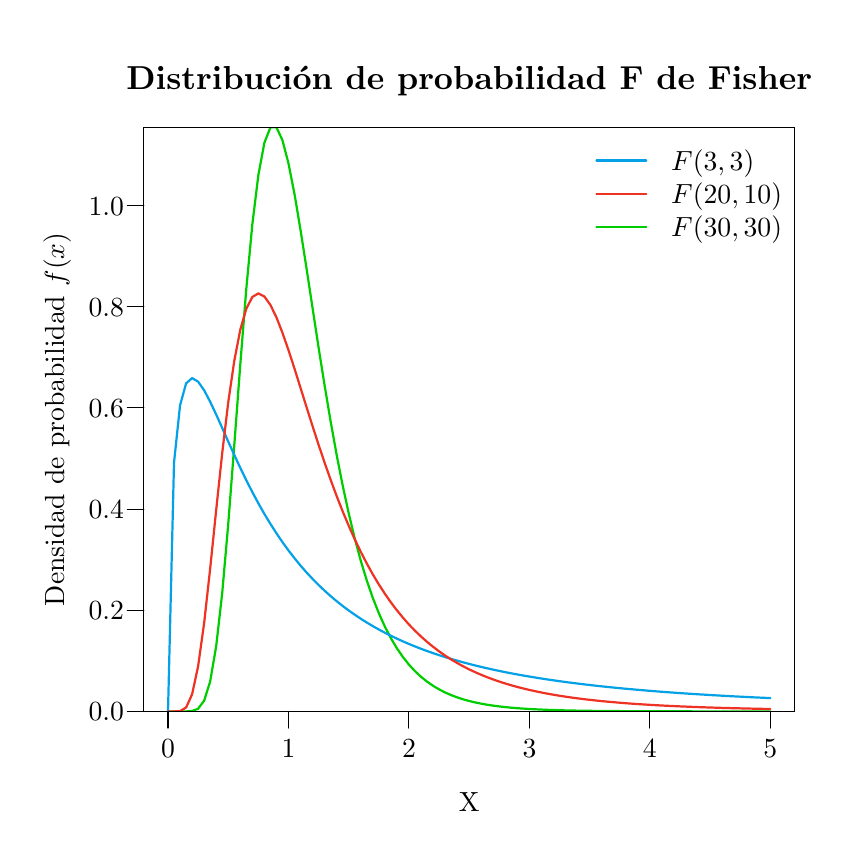
\begin{tikzpicture}[x=1pt,y=1pt]
\definecolor{fillColor}{RGB}{255,255,255}
\path[use as bounding box,fill=fillColor,fill opacity=0.00] (0,0) rectangle (289.08,289.08);
\begin{scope}
\path[clip] ( 42.00, 42.00) rectangle (277.08,253.08);
\definecolor{drawColor}{RGB}{0,205,0}

\path[draw=drawColor,line width= 0.8pt,line join=round,line cap=round] ( 50.71, 42.00) --
	( 52.88, 42.00) --
	( 55.06, 42.00) --
	( 57.24, 42.01) --
	( 59.41, 42.15) --
	( 61.59, 42.98) --
	( 63.77, 45.88) --
	( 65.94, 52.83) --
	( 68.12, 65.59) --
	( 70.30, 84.81) --
	( 72.47,109.69) --
	( 74.65,138.11) --
	( 76.83,167.37) --
	( 79.00,194.73) --
	( 81.18,218.02) --
	( 83.36,235.81) --
	( 85.53,247.47) --
	( 87.71,253.04) --
	( 89.89,253.08) --
	( 92.06,248.42) --
	( 94.24,240.04) --
	( 96.42,228.94) --
	( 98.59,216.01) --
	(100.77,202.06) --
	(102.95,187.72) --
	(105.12,173.50) --
	(107.30,159.77) --
	(109.48,146.78) --
	(111.65,134.71) --
	(113.83,123.63) --
	(116.01,113.57) --
	(118.18,104.53) --
	(120.36, 96.47) --
	(122.54, 89.32) --
	(124.71, 83.02) --
	(126.89, 77.50) --
	(129.07, 72.67) --
	(131.24, 68.47) --
	(133.42, 64.82) --
	(135.60, 61.66) --
	(137.77, 58.92) --
	(139.95, 56.56) --
	(142.13, 54.53) --
	(144.30, 52.78) --
	(146.48, 51.27) --
	(148.66, 49.97) --
	(150.83, 48.86) --
	(153.01, 47.91) --
	(155.19, 47.08) --
	(157.36, 46.38) --
	(159.54, 45.77) --
	(161.72, 45.25) --
	(163.89, 44.81) --
	(166.07, 44.42) --
	(168.25, 44.09) --
	(170.42, 43.81) --
	(172.60, 43.56) --
	(174.78, 43.35) --
	(176.95, 43.17) --
	(179.13, 43.02) --
	(181.31, 42.88) --
	(183.48, 42.77) --
	(185.66, 42.67) --
	(187.84, 42.58) --
	(190.01, 42.50) --
	(192.19, 42.44) --
	(194.37, 42.38) --
	(196.54, 42.33) --
	(198.72, 42.29) --
	(200.90, 42.25) --
	(203.07, 42.22) --
	(205.25, 42.20) --
	(207.43, 42.17) --
	(209.60, 42.15) --
	(211.78, 42.13) --
	(213.96, 42.12) --
	(216.13, 42.10) --
	(218.31, 42.09) --
	(220.49, 42.08) --
	(222.66, 42.07) --
	(224.84, 42.06) --
	(227.02, 42.05) --
	(229.19, 42.05) --
	(231.37, 42.04) --
	(233.55, 42.04) --
	(235.72, 42.03) --
	(237.90, 42.03) --
	(240.08, 42.03) --
	(242.25, 42.02) --
	(244.43, 42.02) --
	(246.61, 42.02) --
	(248.78, 42.02) --
	(250.96, 42.01) --
	(253.14, 42.01) --
	(255.31, 42.01) --
	(257.49, 42.01) --
	(259.67, 42.01) --
	(261.84, 42.01) --
	(264.02, 42.01) --
	(266.20, 42.01) --
	(268.37, 42.01);
\end{scope}
\begin{scope}
\path[clip] (  0.00,  0.00) rectangle (289.08,289.08);
\definecolor{drawColor}{RGB}{0,0,0}

\path[draw=drawColor,line width= 0.4pt,line join=round,line cap=round] ( 50.71, 42.00) -- (268.37, 42.00);

\path[draw=drawColor,line width= 0.4pt,line join=round,line cap=round] ( 50.71, 42.00) -- ( 50.71, 36.00);

\path[draw=drawColor,line width= 0.4pt,line join=round,line cap=round] ( 94.24, 42.00) -- ( 94.24, 36.00);

\path[draw=drawColor,line width= 0.4pt,line join=round,line cap=round] (137.77, 42.00) -- (137.77, 36.00);

\path[draw=drawColor,line width= 0.4pt,line join=round,line cap=round] (181.31, 42.00) -- (181.31, 36.00);

\path[draw=drawColor,line width= 0.4pt,line join=round,line cap=round] (224.84, 42.00) -- (224.84, 36.00);

\path[draw=drawColor,line width= 0.4pt,line join=round,line cap=round] (268.37, 42.00) -- (268.37, 36.00);

\node[text=drawColor,anchor=base,inner sep=0pt, outer sep=0pt, scale=  1.00] at ( 50.71, 25.20) {0};

\node[text=drawColor,anchor=base,inner sep=0pt, outer sep=0pt, scale=  1.00] at ( 94.24, 25.20) {1};

\node[text=drawColor,anchor=base,inner sep=0pt, outer sep=0pt, scale=  1.00] at (137.77, 25.20) {2};

\node[text=drawColor,anchor=base,inner sep=0pt, outer sep=0pt, scale=  1.00] at (181.31, 25.20) {3};

\node[text=drawColor,anchor=base,inner sep=0pt, outer sep=0pt, scale=  1.00] at (224.84, 25.20) {4};

\node[text=drawColor,anchor=base,inner sep=0pt, outer sep=0pt, scale=  1.00] at (268.37, 25.20) {5};

\path[draw=drawColor,line width= 0.4pt,line join=round,line cap=round] ( 42.00, 42.00) -- ( 42.00,224.78);

\path[draw=drawColor,line width= 0.4pt,line join=round,line cap=round] ( 42.00, 42.00) -- ( 36.00, 42.00);

\path[draw=drawColor,line width= 0.4pt,line join=round,line cap=round] ( 42.00, 78.56) -- ( 36.00, 78.56);

\path[draw=drawColor,line width= 0.4pt,line join=round,line cap=round] ( 42.00,115.11) -- ( 36.00,115.11);

\path[draw=drawColor,line width= 0.4pt,line join=round,line cap=round] ( 42.00,151.67) -- ( 36.00,151.67);

\path[draw=drawColor,line width= 0.4pt,line join=round,line cap=round] ( 42.00,188.23) -- ( 36.00,188.23);

\path[draw=drawColor,line width= 0.4pt,line join=round,line cap=round] ( 42.00,224.78) -- ( 36.00,224.78);

\node[text=drawColor,anchor=base east,inner sep=0pt, outer sep=0pt, scale=  1.00] at ( 34.80, 38.56) {0.0};

\node[text=drawColor,anchor=base east,inner sep=0pt, outer sep=0pt, scale=  1.00] at ( 34.80, 75.11) {0.2};

\node[text=drawColor,anchor=base east,inner sep=0pt, outer sep=0pt, scale=  1.00] at ( 34.80,111.67) {0.4};

\node[text=drawColor,anchor=base east,inner sep=0pt, outer sep=0pt, scale=  1.00] at ( 34.80,148.23) {0.6};

\node[text=drawColor,anchor=base east,inner sep=0pt, outer sep=0pt, scale=  1.00] at ( 34.80,184.78) {0.8};

\node[text=drawColor,anchor=base east,inner sep=0pt, outer sep=0pt, scale=  1.00] at ( 34.80,221.34) {1.0};

\path[draw=drawColor,line width= 0.4pt,line join=round,line cap=round] ( 42.00, 42.00) --
	(277.08, 42.00) --
	(277.08,253.08) --
	( 42.00,253.08) --
	( 42.00, 42.00);
\end{scope}
\begin{scope}
\path[clip] (  0.00,  0.00) rectangle (289.08,289.08);
\definecolor{drawColor}{RGB}{0,0,0}

\node[text=drawColor,anchor=base,inner sep=0pt, outer sep=0pt, scale=  1.20] at (159.54,266.89) {\bfseries Distribución de probabilidad F de Fisher};

\node[text=drawColor,anchor=base,inner sep=0pt, outer sep=0pt, scale=  1.00] at (159.54,  6.00) {X};

\node[text=drawColor,rotate= 90.00,anchor=base,inner sep=0pt, outer sep=0pt, scale=  1.00] at ( 13.20,147.54) {Densidad de probabilidad $f(x)$};
\end{scope}
\begin{scope}
\path[clip] ( 42.00, 42.00) rectangle (277.08,253.08);
\definecolor{drawColor}{RGB}{5,161,230}

\path[draw=drawColor,line width= 0.8pt,line join=round,line cap=round] ( 50.71, 42.00) --
	( 52.88,131.91) --
	( 55.06,152.59) --
	( 57.24,160.53) --
	( 59.41,162.46) --
	( 61.59,161.16) --
	( 63.77,158.04) --
	( 65.94,153.92) --
	( 68.12,149.28) --
	( 70.30,144.42) --
	( 72.47,139.52) --
	( 74.65,134.70) --
	( 76.83,130.02) --
	( 79.00,125.54) --
	( 81.18,121.26) --
	( 83.36,117.21) --
	( 85.53,113.38) --
	( 87.71,109.78) --
	( 89.89,106.38) --
	( 92.06,103.18) --
	( 94.24,100.18) --
	( 96.42, 97.36) --
	( 98.59, 94.71) --
	(100.77, 92.22) --
	(102.95, 89.89) --
	(105.12, 87.69) --
	(107.30, 85.62) --
	(109.48, 83.67) --
	(111.65, 81.84) --
	(113.83, 80.11) --
	(116.01, 78.48) --
	(118.18, 76.95) --
	(120.36, 75.50) --
	(122.54, 74.13) --
	(124.71, 72.83) --
	(126.89, 71.61) --
	(129.07, 70.45) --
	(131.24, 69.35) --
	(133.42, 68.31) --
	(135.60, 67.32) --
	(137.77, 66.38) --
	(139.95, 65.49) --
	(142.13, 64.64) --
	(144.30, 63.84) --
	(146.48, 63.07) --
	(148.66, 62.34) --
	(150.83, 61.64) --
	(153.01, 60.98) --
	(155.19, 60.35) --
	(157.36, 59.74) --
	(159.54, 59.17) --
	(161.72, 58.61) --
	(163.89, 58.09) --
	(166.07, 57.58) --
	(168.25, 57.10) --
	(170.42, 56.64) --
	(172.60, 56.19) --
	(174.78, 55.77) --
	(176.95, 55.36) --
	(179.13, 54.97) --
	(181.31, 54.60) --
	(183.48, 54.24) --
	(185.66, 53.89) --
	(187.84, 53.56) --
	(190.01, 53.24) --
	(192.19, 52.93) --
	(194.37, 52.63) --
	(196.54, 52.35) --
	(198.72, 52.08) --
	(200.90, 51.81) --
	(203.07, 51.56) --
	(205.25, 51.31) --
	(207.43, 51.07) --
	(209.60, 50.84) --
	(211.78, 50.62) --
	(213.96, 50.41) --
	(216.13, 50.20) --
	(218.31, 50.01) --
	(220.49, 49.81) --
	(222.66, 49.63) --
	(224.84, 49.45) --
	(227.02, 49.27) --
	(229.19, 49.10) --
	(231.37, 48.94) --
	(233.55, 48.78) --
	(235.72, 48.63) --
	(237.90, 48.48) --
	(240.08, 48.34) --
	(242.25, 48.20) --
	(244.43, 48.07) --
	(246.61, 47.93) --
	(248.78, 47.81) --
	(250.96, 47.68) --
	(253.14, 47.56) --
	(255.31, 47.45) --
	(257.49, 47.34) --
	(259.67, 47.23) --
	(261.84, 47.12) --
	(264.02, 47.02) --
	(266.20, 46.92) --
	(268.37, 46.82);
\definecolor{drawColor}{RGB}{238,50,36}

\path[draw=drawColor,line width= 0.8pt,line join=round,line cap=round] ( 50.71, 42.00) --
	( 52.88, 42.00) --
	( 55.06, 42.12) --
	( 57.24, 43.41) --
	( 59.41, 48.17) --
	( 61.59, 58.32) --
	( 63.77, 73.99) --
	( 65.94, 93.59) --
	( 68.12,114.80) --
	( 70.30,135.39) --
	( 72.47,153.67) --
	( 74.65,168.66) --
	( 76.83,179.94) --
	( 79.00,187.54) --
	( 81.18,191.76) --
	( 83.36,193.05) --
	( 85.53,191.93) --
	( 87.71,188.89) --
	( 89.89,184.39) --
	( 92.06,178.84) --
	( 94.24,172.57) --
	( 96.42,165.87) --
	( 98.59,158.94) --
	(100.77,151.96) --
	(102.95,145.07) --
	(105.12,138.35) --
	(107.30,131.87) --
	(109.48,125.69) --
	(111.65,119.82) --
	(113.83,114.28) --
	(116.01,109.08) --
	(118.18,104.22) --
	(120.36, 99.68) --
	(122.54, 95.46) --
	(124.71, 91.54) --
	(126.89, 87.90) --
	(129.07, 84.54) --
	(131.24, 81.42) --
	(133.42, 78.55) --
	(135.60, 75.89) --
	(137.77, 73.43) --
	(139.95, 71.17) --
	(142.13, 69.08) --
	(144.30, 67.15) --
	(146.48, 65.37) --
	(148.66, 63.72) --
	(150.83, 62.20) --
	(153.01, 60.80) --
	(155.19, 59.50) --
	(157.36, 58.31) --
	(159.54, 57.20) --
	(161.72, 56.18) --
	(163.89, 55.23) --
	(166.07, 54.35) --
	(168.25, 53.54) --
	(170.42, 52.79) --
	(172.60, 52.09) --
	(174.78, 51.44) --
	(176.95, 50.84) --
	(179.13, 50.29) --
	(181.31, 49.77) --
	(183.48, 49.29) --
	(185.66, 48.84) --
	(187.84, 48.42) --
	(190.01, 48.03) --
	(192.19, 47.67) --
	(194.37, 47.33) --
	(196.54, 47.02) --
	(198.72, 46.73) --
	(200.90, 46.45) --
	(203.07, 46.20) --
	(205.25, 45.96) --
	(207.43, 45.73) --
	(209.60, 45.52) --
	(211.78, 45.33) --
	(213.96, 45.15) --
	(216.13, 44.97) --
	(218.31, 44.81) --
	(220.49, 44.66) --
	(222.66, 44.52) --
	(224.84, 44.39) --
	(227.02, 44.26) --
	(229.19, 44.14) --
	(231.37, 44.03) --
	(233.55, 43.93) --
	(235.72, 43.83) --
	(237.90, 43.74) --
	(240.08, 43.65) --
	(242.25, 43.57) --
	(244.43, 43.49) --
	(246.61, 43.42) --
	(248.78, 43.35) --
	(250.96, 43.28) --
	(253.14, 43.22) --
	(255.31, 43.16) --
	(257.49, 43.11) --
	(259.67, 43.06) --
	(261.84, 43.01) --
	(264.02, 42.96) --
	(266.20, 42.92) --
	(268.37, 42.88);
\definecolor{drawColor}{RGB}{5,161,230}

\path[draw=drawColor,line width= 0.8pt,line join=round,line cap=round] (205.54,241.08) -- (223.54,241.08);
\definecolor{drawColor}{RGB}{238,50,36}

\path[draw=drawColor,line width= 0.8pt,line join=round,line cap=round] (205.54,229.08) -- (223.54,229.08);
\definecolor{drawColor}{RGB}{0,205,0}

\path[draw=drawColor,line width= 0.8pt,line join=round,line cap=round] (205.54,217.08) -- (223.54,217.08);
\definecolor{drawColor}{RGB}{0,0,0}

\node[text=drawColor,anchor=base west,inner sep=0pt, outer sep=0pt, scale=  1.00] at (232.54,237.64) {$F(3,3)$};

\node[text=drawColor,anchor=base west,inner sep=0pt, outer sep=0pt, scale=  1.00] at (232.54,225.64) {$F(20,10)$};

\node[text=drawColor,anchor=base west,inner sep=0pt, outer sep=0pt, scale=  1.00] at (232.54,213.64) {$F(30,30)$};
\end{scope}
\begin{scope}
\path[clip] (  0.00,  0.00) rectangle (289.08,289.08);
\definecolor{drawColor}{RGB}{0,0,0}

\path[draw=drawColor,line width= 0.4pt,line join=round,line cap=round] ( 42.00, 42.00) --
	(277.08, 42.00) --
	(277.08,253.08) --
	( 42.00,253.08) --
	( 42.00, 42.00);
\end{scope}
\end{tikzpicture}
}
\end{center}

\note{
Aquí tenemos las gráfica de la función de densidad de varias distribuciones F de Fisher con distintos grados de libertad. Como se puede
apreciar, al igual que la distribución chi-cuadrado, no presenta valores negativos, y siempre es asimétrica hacia la izquierda.
}
\end{frame}


%---------------------------------------------------------------------slide----
\begin{frame}
\frametitle{Propiedades de la distribución F de Fisher-Snedecor $F(m,n)$}
\begin{itemize}
\item No está definida para valores negativos.
\item De la definición se deduce que
\[
F(m,n) =\frac{1}{F(n,m)}
\]
de manera que si llamamos $f(m,n)_p$ al valor que cumple que $P(F(m,n)≤f(m,n)_p)=p$, entonces se cumple
\[                                          
f(m,n)_p =\frac{1}{f(n,m)_{1−p}}
\]
Esto resulta muy útil para utilizar las tablas de su función de distribución.
\end{itemize}

\note{
Algunas propiedades que tiene la distribución F de Fisher son:
\begin{itemize}
\item No está definida para valores negativos.
\item De la definición se deduce que
\[
F(m,n) =\frac{1}{F(n,m)}
\]
de manera que si llamamos $f(m,n)_p$ al valor que cumple que $P(F(m,n)≤f(m,n)_p)=p$, entonces se cumple
\[                                          
f(m,n)_p =\frac{1}{f(n,m)_{1−p}}
\]
Esto resulta muy útil para utilizar las tablas de su función de distribución.
\end{itemize}
}
\end{frame}
